
\documentclass[11pt,a4paper]{article}
\usepackage[hyperref]{acl2020}
\usepackage{times}
\usepackage{latexsym}
\renewcommand{\UrlFont}{\ttfamily\small}

\usepackage{microtype}

\usepackage{verbatim}

\usepackage{amsmath}
\usepackage{listings}
\usepackage{amsfonts}

\usepackage{graphicx}
\usepackage{multirow}
\usepackage{array}
\usepackage{booktabs}

\usepackage{url}
\makeatletter

\newcommand{\printfnsymbol}[1]{%
  \textsuperscript{\@fnsymbol{#1}}%
}

\makeatother

\aclfinalcopy % Uncomment this line for the final submission

%\setlength\titlebox{5cm}
% You can expand the titlebox if you need extra space
% to show all the authors. Please do not make the titlebox
% smaller than 5cm (the original size); we will check this
% in the camera-ready version and ask you to change it back.


\newcommand\BibTeX{B\textsc{ib}\TeX}

\title{CraftAssist Instruction Parsing: Semantic Parsing for a Voxel-World Assistant}

%{Kavya Srinet  \\
%  Facebook AI Research / Address line 1 \\
%  Affiliation / Address line 2 \\
%  Affiliation / Address line 3 \\
%  {\tt ksrinet@fb.com} \\\And
%  Yacine Jernite \\
%  Affiliation / Address line 1 \\
%  Affiliation / Address line 2 \\
%  Affiliation / Address line 3 \\
%  {\tt email@domain} \\}

\author{Kavya Srinet\thanks{ equal contribution} \\
  Facebook AI Research  \\
  {\texttt{ksrinet@fb.com} }\\\And
  Yacine Jernite\printfnsymbol{1}\thanks{Work done while at Facebook AI Research} \\
  HuggingFace  \\ 
  {\texttt{yacine@}}\\
  {\texttt{ huggingface.co} }\\\And
  Jonathan Gray \\
  Facebook AI Research  \\
  {\texttt{jsgray@fb.com}} \\\And
  Arthur Szlam \\
  Facebook AI Research  \\
  {\texttt{aszlam@fb.com} }\\}
  

\date{}

\begin{document}

\maketitle
\begin{abstract}
We propose a semantic parsing dataset focused on instruction-driven communication with an agent in the game Minecraft\footnote{Minecraft features: \textcopyright Mojang Synergies AB included courtesy of Mojang AB}.  
%The dataset consists of 32K human generated instructions with their parses, derived from a large collection of templates.   
The dataset consists of 
%several thousand templates that can synthesize surface forms and their parses, and
 ~7K human utterances and their corresponding parses.  Given proper world state, the parses can be interpreted and executed in game. 
We report the performance of baseline models, and analyze their successes and failures.
% and find that while we are able to train a usable interface with the agent, there is 
 % dataset reveals interesting generalization challenges.
\end{abstract}

\section{Introduction} 
Semantic parsing is used as a component for natural language understanding in human-robot interaction systems \cite{lauria2001training, bos2007spoken, tellex2011understanding, matuszek2013learning, thomason2019improving}, and for virtual assistants  \cite{kollar2018alexa}.  We would like to be able to apply deep learning methods in this space, as recently researchers have shown success with these methods for semantic parsing more generally, e.g. \cite{dong2016language, jia2016data, zhong2017seq2sql}. However, to fully utilize powerful neural network approaches, it is necessary to have large numbers of training examples. In the space of human-robot (or human-assistant) interaction, the publicly available semantic parsing datasets are small. Furthermore, it can be difficult to reproduce the end-to-end results (from utterance to action in the environment) because of the wide variety of robot setups and proprietary nature of personal assistants.

In this work, we introduce a new semantic parsing dataset for human-bot interactions. Our ``robot'' or ``assistant''  is embodied in the sandbox construction game Minecraft\footnote{\url{https://minecraft.net/en-us/}.  We limit ourselves to creative mode for this work}, a popular multiplayer open-world voxel-based crafting game. We also provide the associated platform for executing the logical forms in game.

Situating the assistant in Minecraft has several benefits for studying task oriented natural language understanding (NLU). Compared to physical robots, Minecraft allows less technical overhead irrelevant to NLU, such as difficulties with hardware and large scale data collection. On the other hand, our bot has all the basic in-game capabilities of a player, including movement and placing or removing voxels. Thus Minecraft preserves many of the NLU elements of physical robots, such as discussions of navigation and spatial object reference. 
 
%\begin{figure*}[t!]
%    \centering
%%     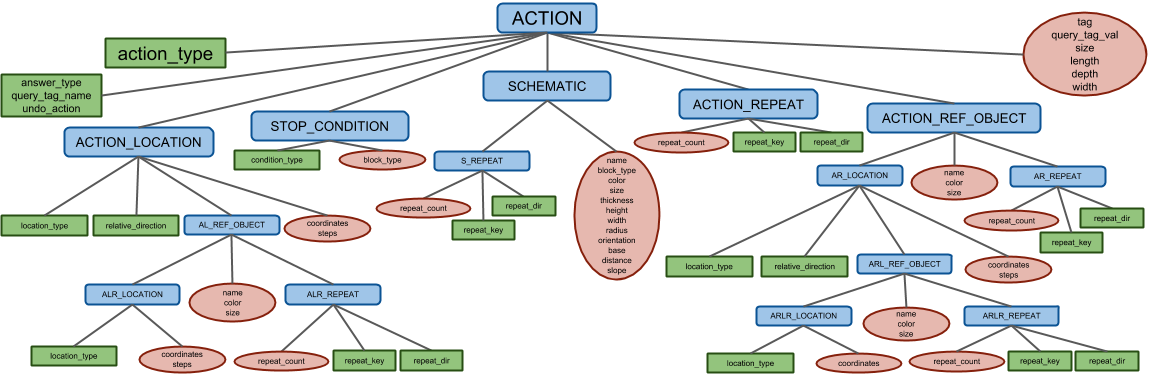
\includegraphics[natwidth=\linewidth]{figures/ActionGrammar.png}
%    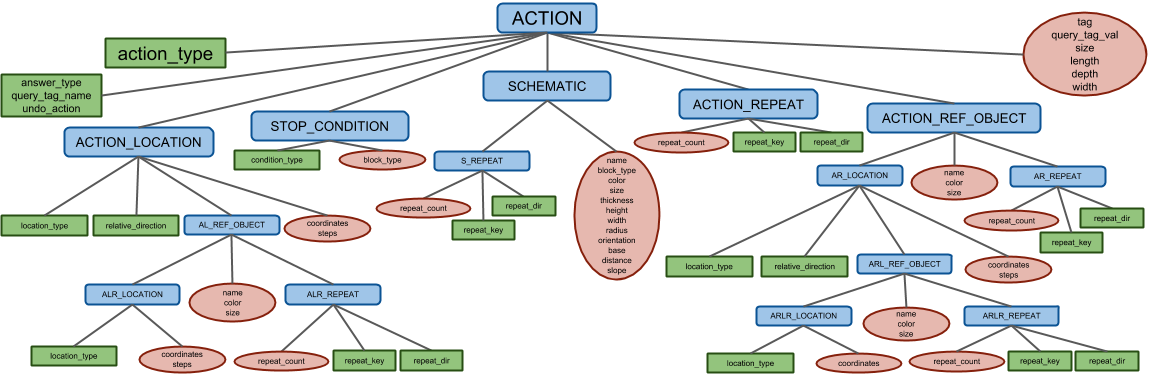
\includegraphics[width=\linewidth]{figures/ActionGrammar.png}
%    \caption{Action space grammar}
%    \label{fig:action_grammar}
%\end{figure*}  


Working in Minecraft may enable large scale human interaction because of its large player base, in the tens of millions. 
 %Compared with personal assistants, Minecraft offers a low
% for allows the possibility of interacting with large number of players
Furthermore, although Minecraft's simulation of physics is simplified, the task space is complex. 
While there are many atomic objects in the game, such as animals and block-types, that require no perceptual modeling, the player also interacts with complex structures made up of collections of voxels such as a ``house'' or a ``hill''. The assistant cannot apprehend them without a perceptual system, creating an ideal test bed for researchers interested in the interactions between perception and language. 

Our contributions in the paper are as follows:
\newline
\noindent{\bf Grammar:} We develop a grammar over a set of primitives that comprise a mid-level interface to Minecraft for machine learning agents.  %See Section \ref{sec:grammar}.
\newline 
\noindent{\bf Data:} %Using a collection of templates to convert logical forms over the primitives into pseudo-natural language, we build a dataset of language instructions with logical form annotation.
% by having crowd-sourced workers rephrase the language outputs, as in \cite{wang2015building}.  
We collect ~7K  crowd-sourced annotations of commands generated independent of our grammar. %, see Section \ref{sec:data}. 
In addition to the natural language commands and the associated logical forms, we release the tools used to collect these, which allow crowd-workers to efficiently and accurately annotate parses.%; see Section \ref{sec:annotation}.
%We hope in addition to use as a semantic parsing dataset, these will be useful for researchers in reinforcement learning.
\newline   
\noindent{\bf Models:} We show the results of several neural semantic parsing models trained on our data. %See Section \ref{sec:modeling} and \ref{sec:experiments}.
\newline   
\noindent{\bf Execution:} Finally, we also make available the code to execute logical forms in the game, allowing the reproduction of end-to-end results.  This also opens the door to using the data for reinforcement and imitation learning with language.
We also provide access to an interactive bot using these models for parsing\footnote{Instructions can be found at \url{http://craftassist.io/acl2020demo}, requires a Minecraft license and client.}. %We demonstrate  that adapting the neural architecture to the grammar can improve parsing accuracy.

%\begin{figure*}[t!]
 %   \centering
%%    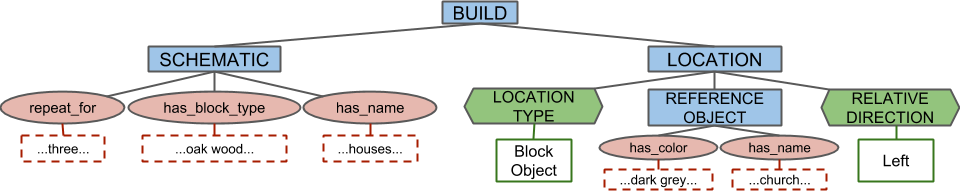
\includegraphics[natwidth=\linewidth ]{figures/ExampleParse.png}
 %   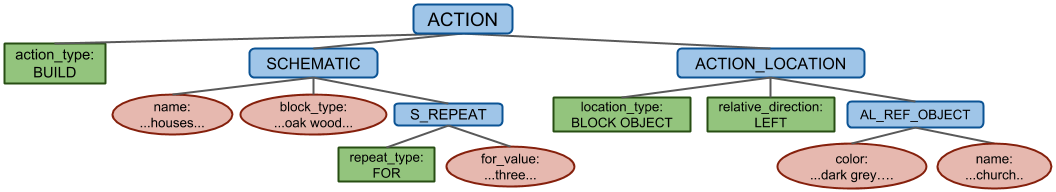
\includegraphics[width=\linewidth ]{figures/ExampleParseNew.png}
 %   \caption{Parse tree for ``Make three oak wood houses to the left of the dark grey church.''    \label{fig:example_parse}
%}
%\end{figure*}


%Advantages of working with MC / game environment -- General usefulness of a large semantic parsing dataset in the context of a semi-tractable virtual environment.


\section{The Assistant Grammar}
\label{sec:grammar}
\begin{figure}
	\centering
     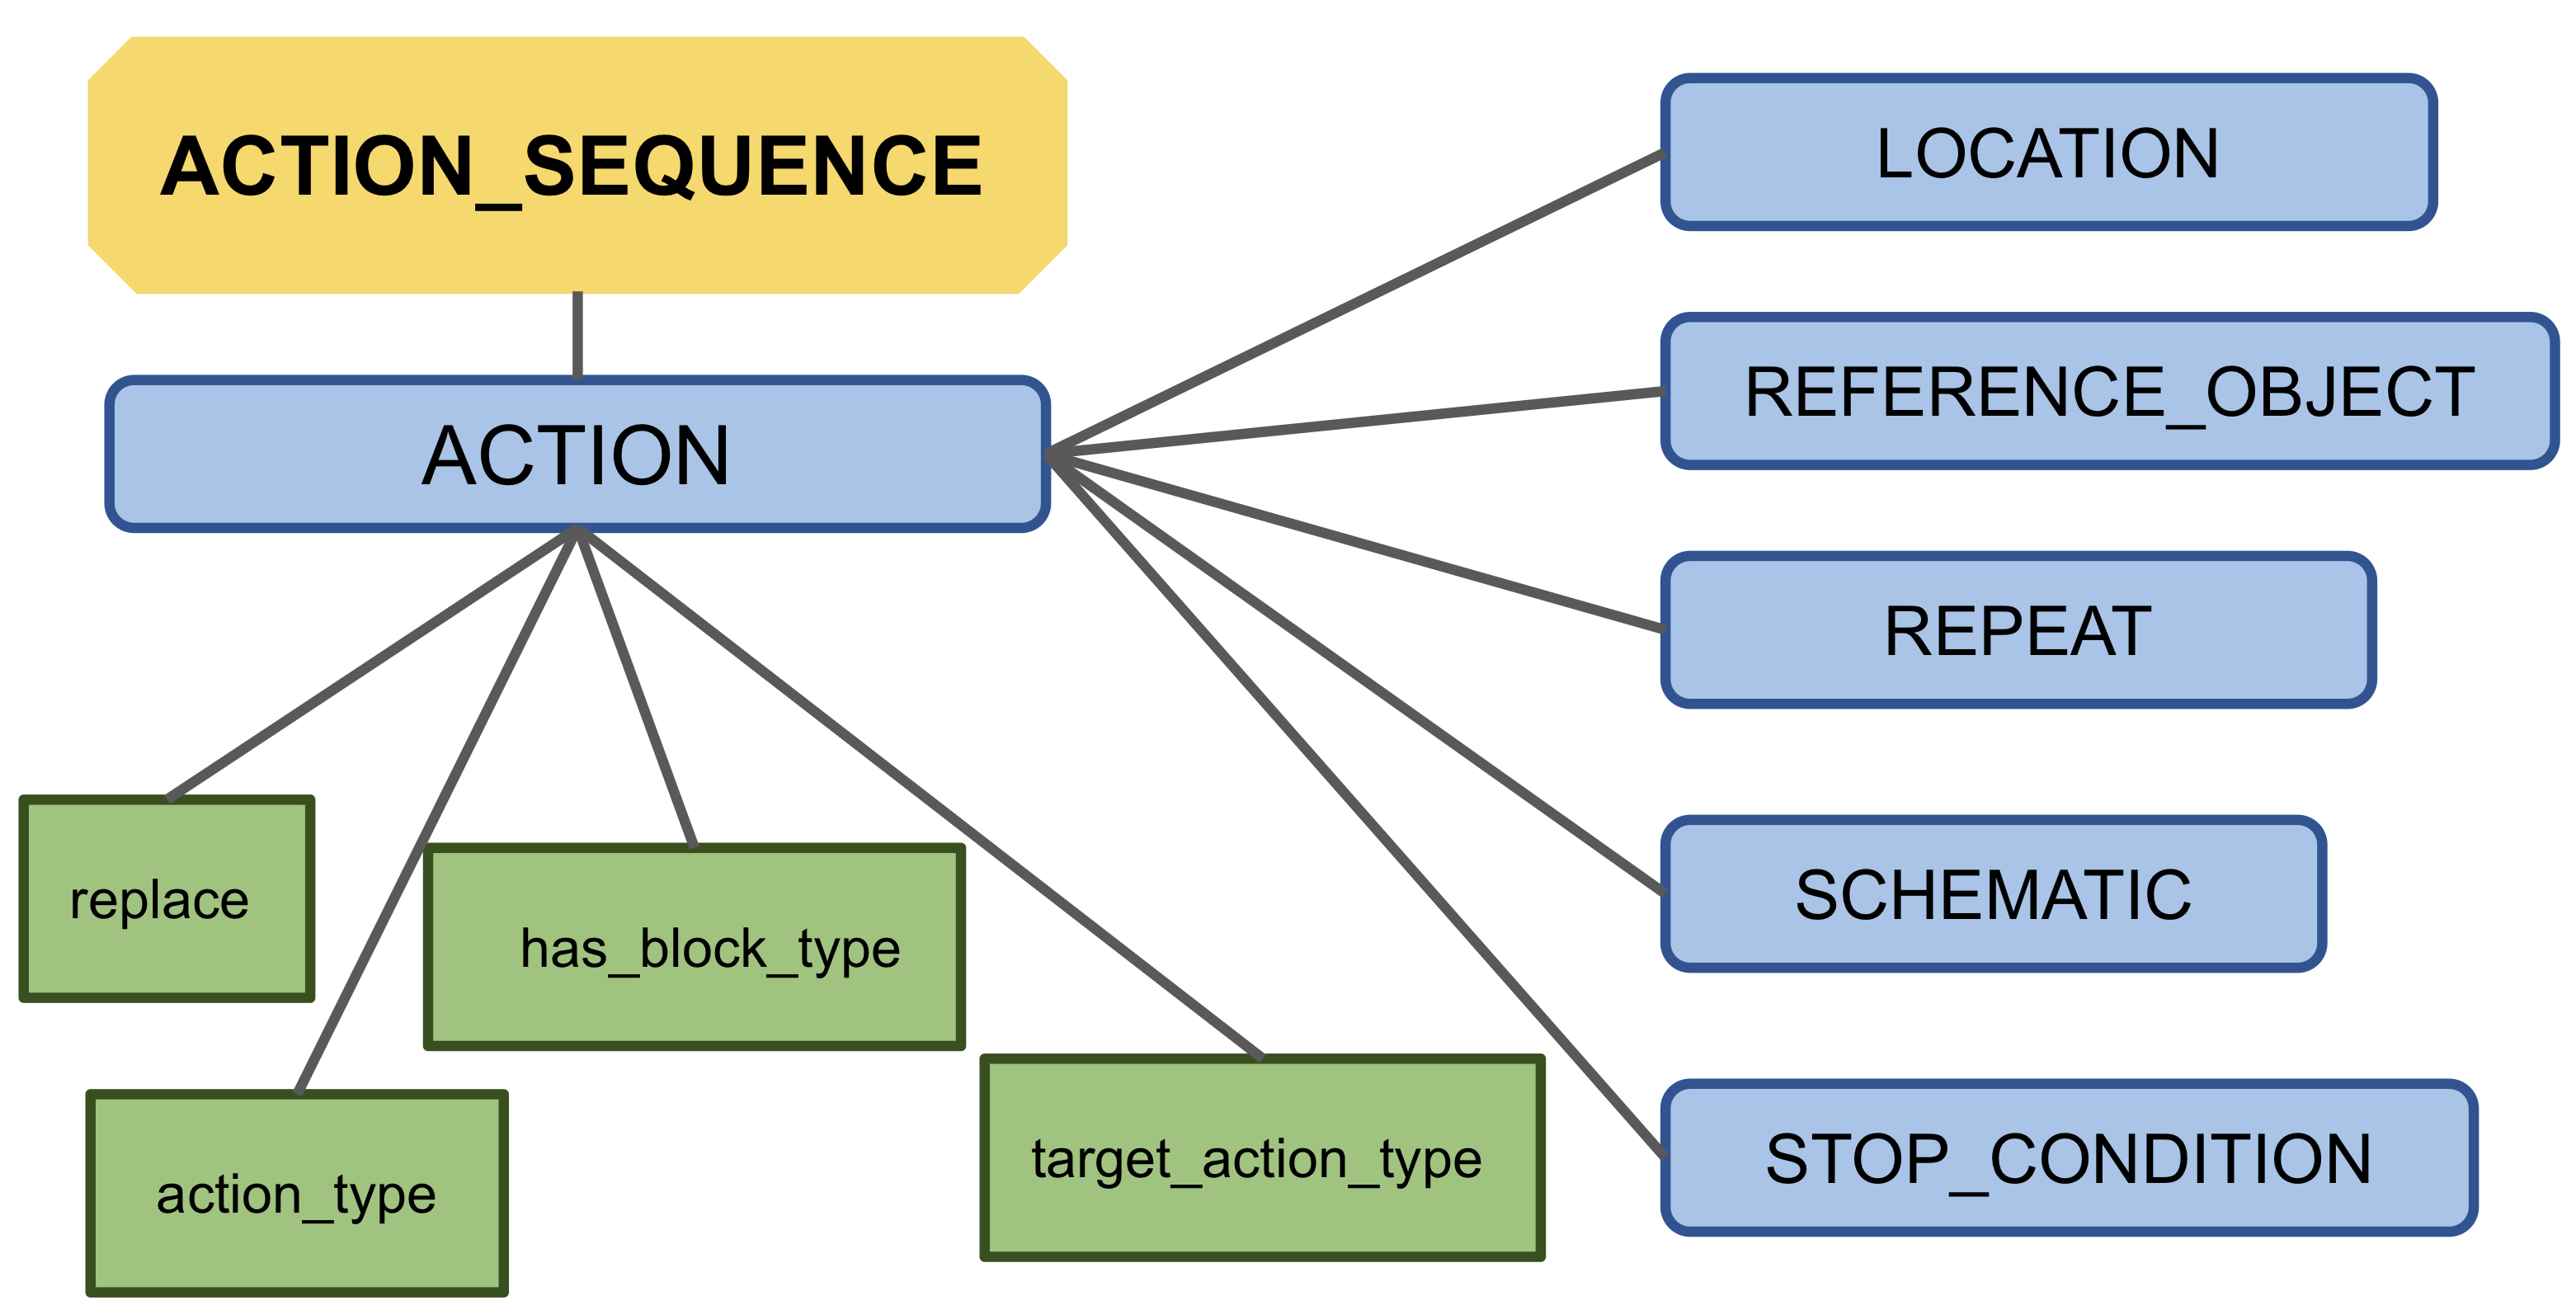
\includegraphics[width=.72\linewidth ]{figures/AS.png}

    \caption{The basic structure of the \textsc{action\_sequence} branch of the assistant's grammar.   The gold octagon is an internal node whose children are ordered,  blue rectangles are regular internal nodes,  and green rectangles are categorical leaf nodes.   Not all combinations of children of \textsc{action} are possible, see the full list of possible productions (and the productions for \textsc{put\_memory} and \textsc{get\_memory})  in the Appendix.}
    \label{fig:AS}
    
\end{figure}


 In this section we summarize a grammar for generating logical forms that can be interpreted into programs for the agent architecture described in \cite{gray2019craftassist}.

\subsection{Agent Action Space}
The assistant's basic functions include moving, and placing and destroying blocks.  Supporting these basic functions are methods for control flow and memory manipulation.  

\smallskip

\noindent{\bf Basic action commands: } The assistant can \textsc{move} to a specified location; or \textsc{dance} with a specified sequence of steps.  It can \textsc{build} an object from a known schematic (or by making a copy of a block-object in the world) at a given location, or \textsc{destroy} an existing object.  It can \textsc{dig} a hole of a given shape at a specified location, or \textsc{fill} one up. The agent can also be asked to complete a partially built structure however it sees fit by \textsc{freebuild}.  Finally, it can \textsc{spawn} a mob (an animate NPC in Minecraft).    

\smallskip

\noindent{\bf Control commands: } Additionally, the agent can \textsc{stop} or \textsc{resume} an action, or \textsc{undo} the result of a recent command.   Furthermore, the assistant can \textsc{loop} given a task and a stop-condition. Finally, it needs to be able to understand when a sentence does not correspond to any of the above mentioned actions, and map it to a \textsc{noop}.

\begin{figure}
    \centering
    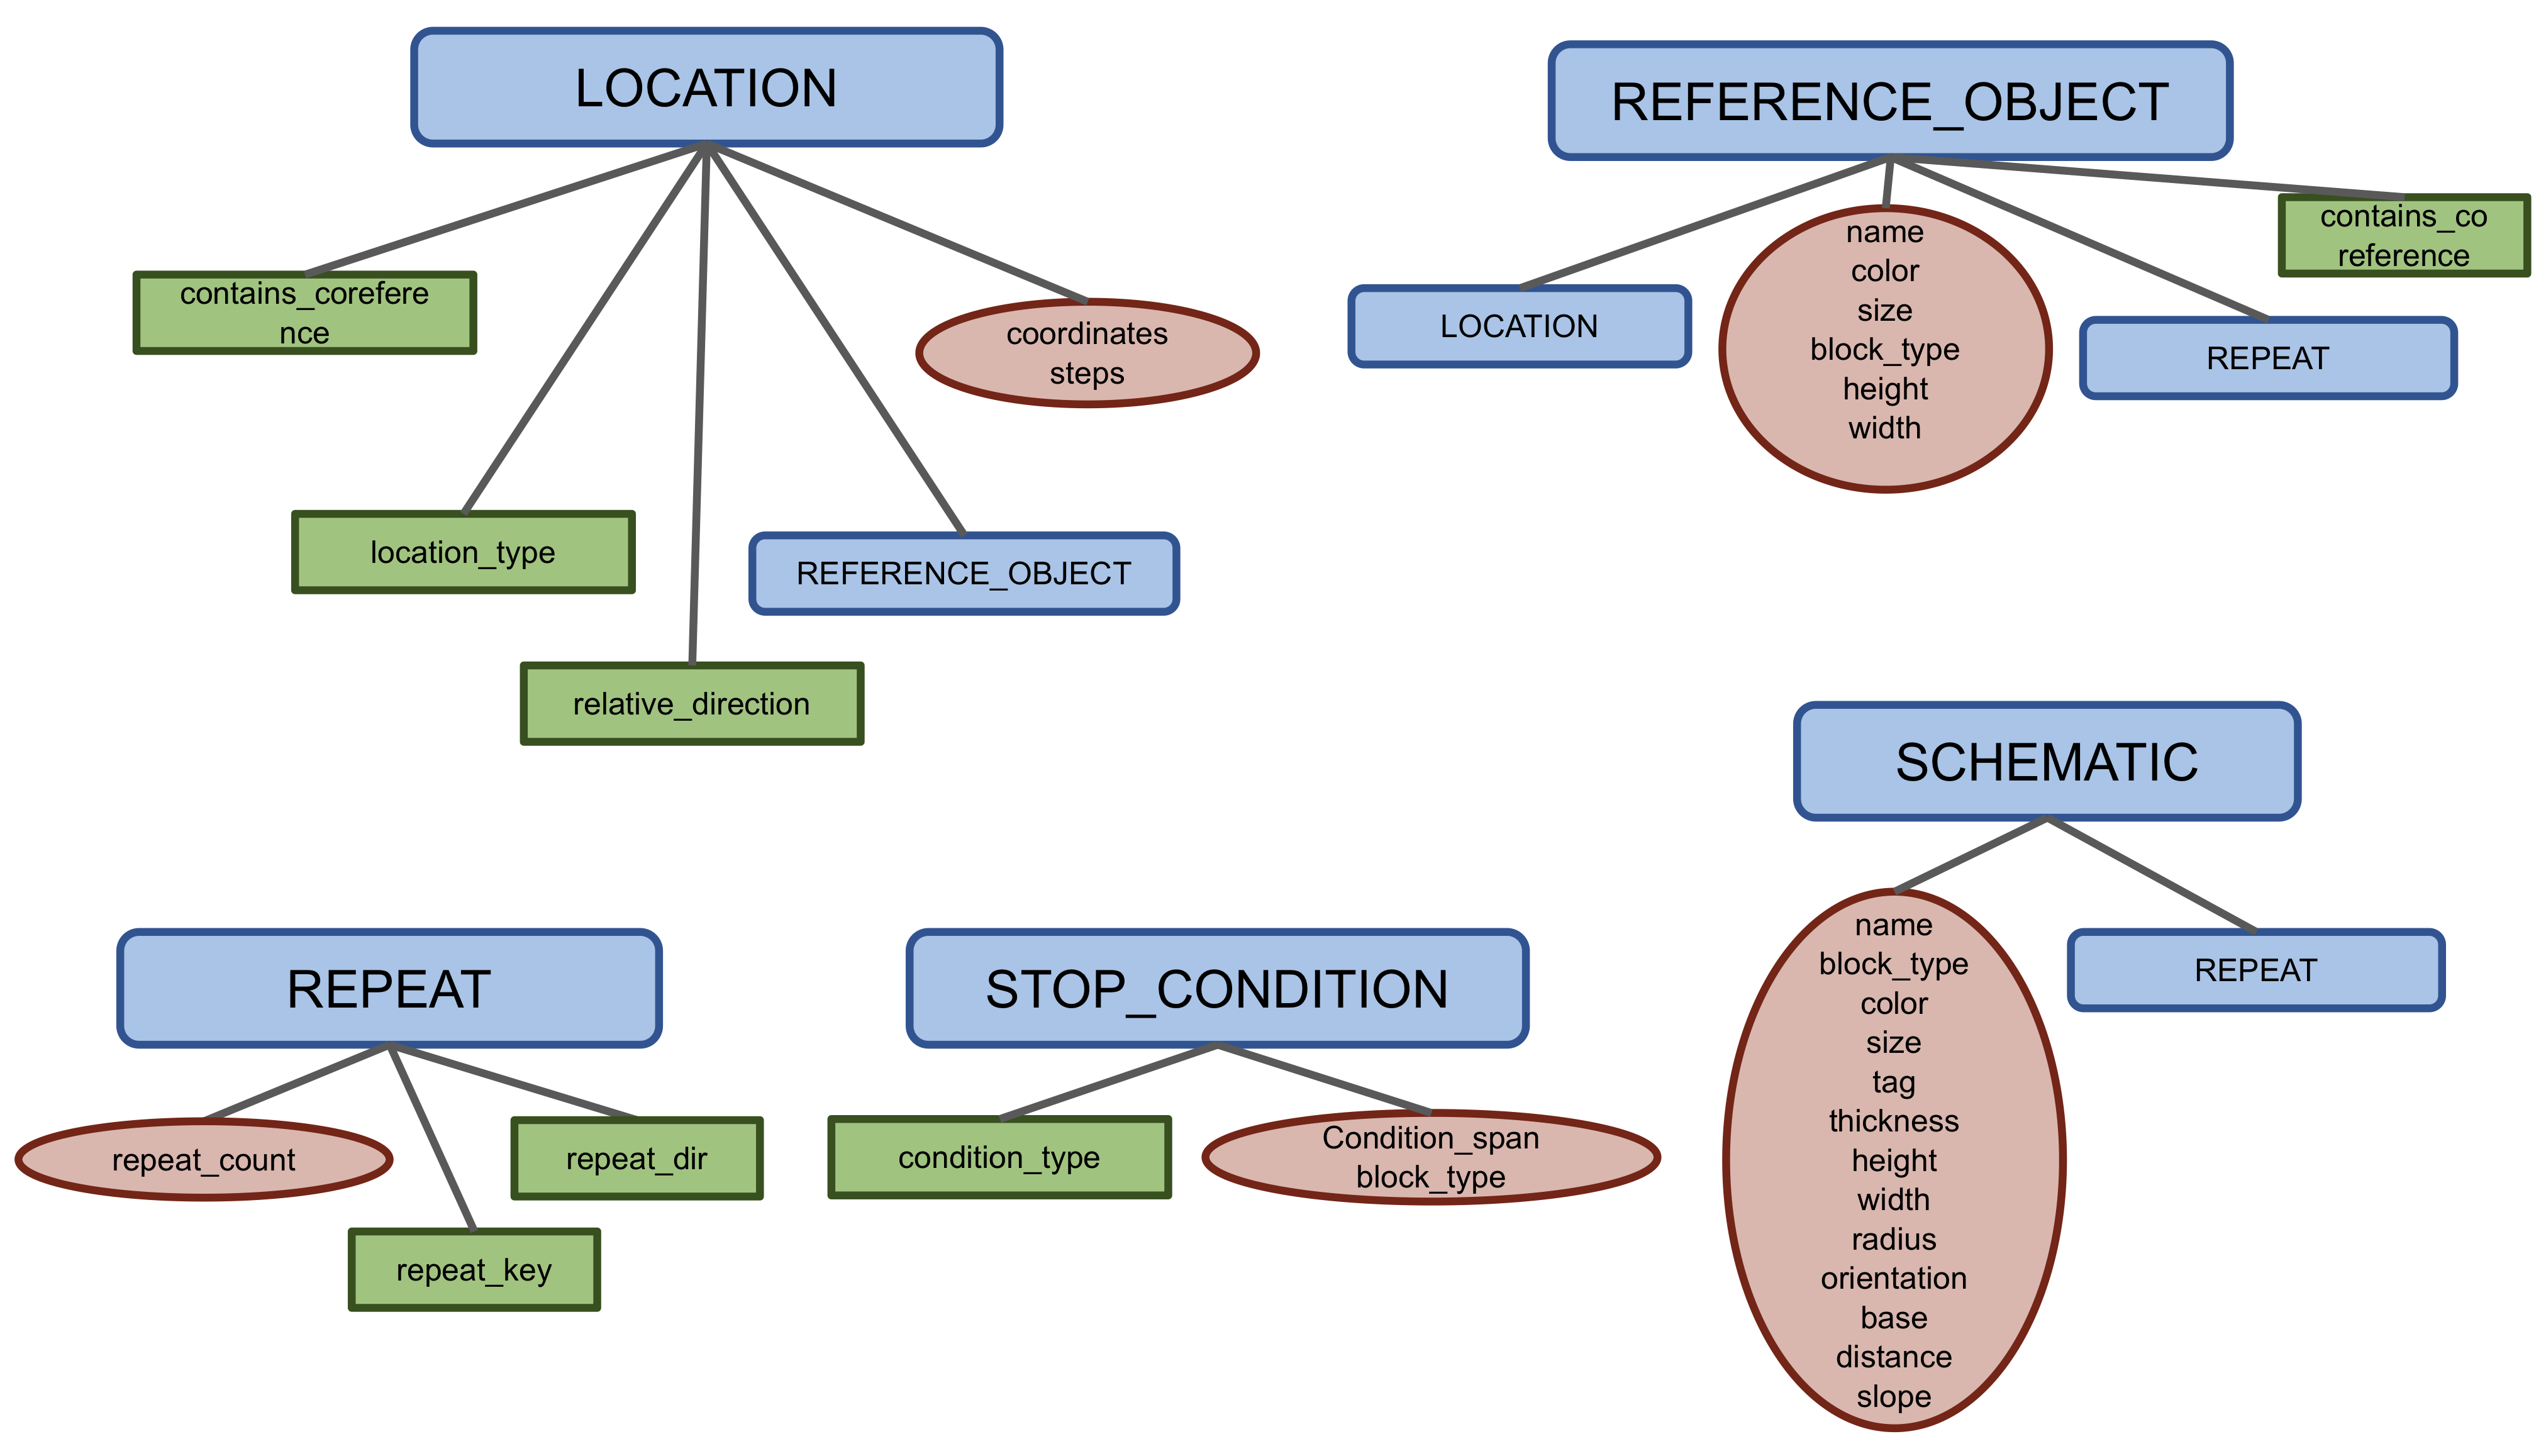
\includegraphics[width=\linewidth, height=6cm ]{figures/NOT_AS.png}
    \caption{The basic structure of internal nodes in the assistant's grammar.   Blue rectangles are internal nodes,  green rectangles are categorical leaf nodes, and red ovals are span nodes.      \label{fig:NOT_AS}}
\end{figure}

\smallskip

\noindent{\bf Memory interface: }  Finally, the assistant can interact with its SQL based memory.  It can place or update rows or cells, for example for tagging objects.  This can be considered a basic version of the self-improvement capabilities in \cite{kollar2013toward, thomason2015learning, wang2016learning, wang2017naturalizing}.    It can retrieve information for question answering similar to the VQA in \cite{yi2018neural}.

% We want to be able to add to this representation by allowing the user to \textsc{tag} existing objects with names or properties.  This can be considered a basic version of the self-improvement capabilities in \cite{kollar2013toward, thomason2015learning, wang2016learning, wang2017naturalizing}. Conversely, to query this internal state, we can ask the agent to \textsc{answer} questions about the world.  This part of the grammar is similar to the visual question-answering in \cite{yi2018neural}

\begin{figure*}
\center
 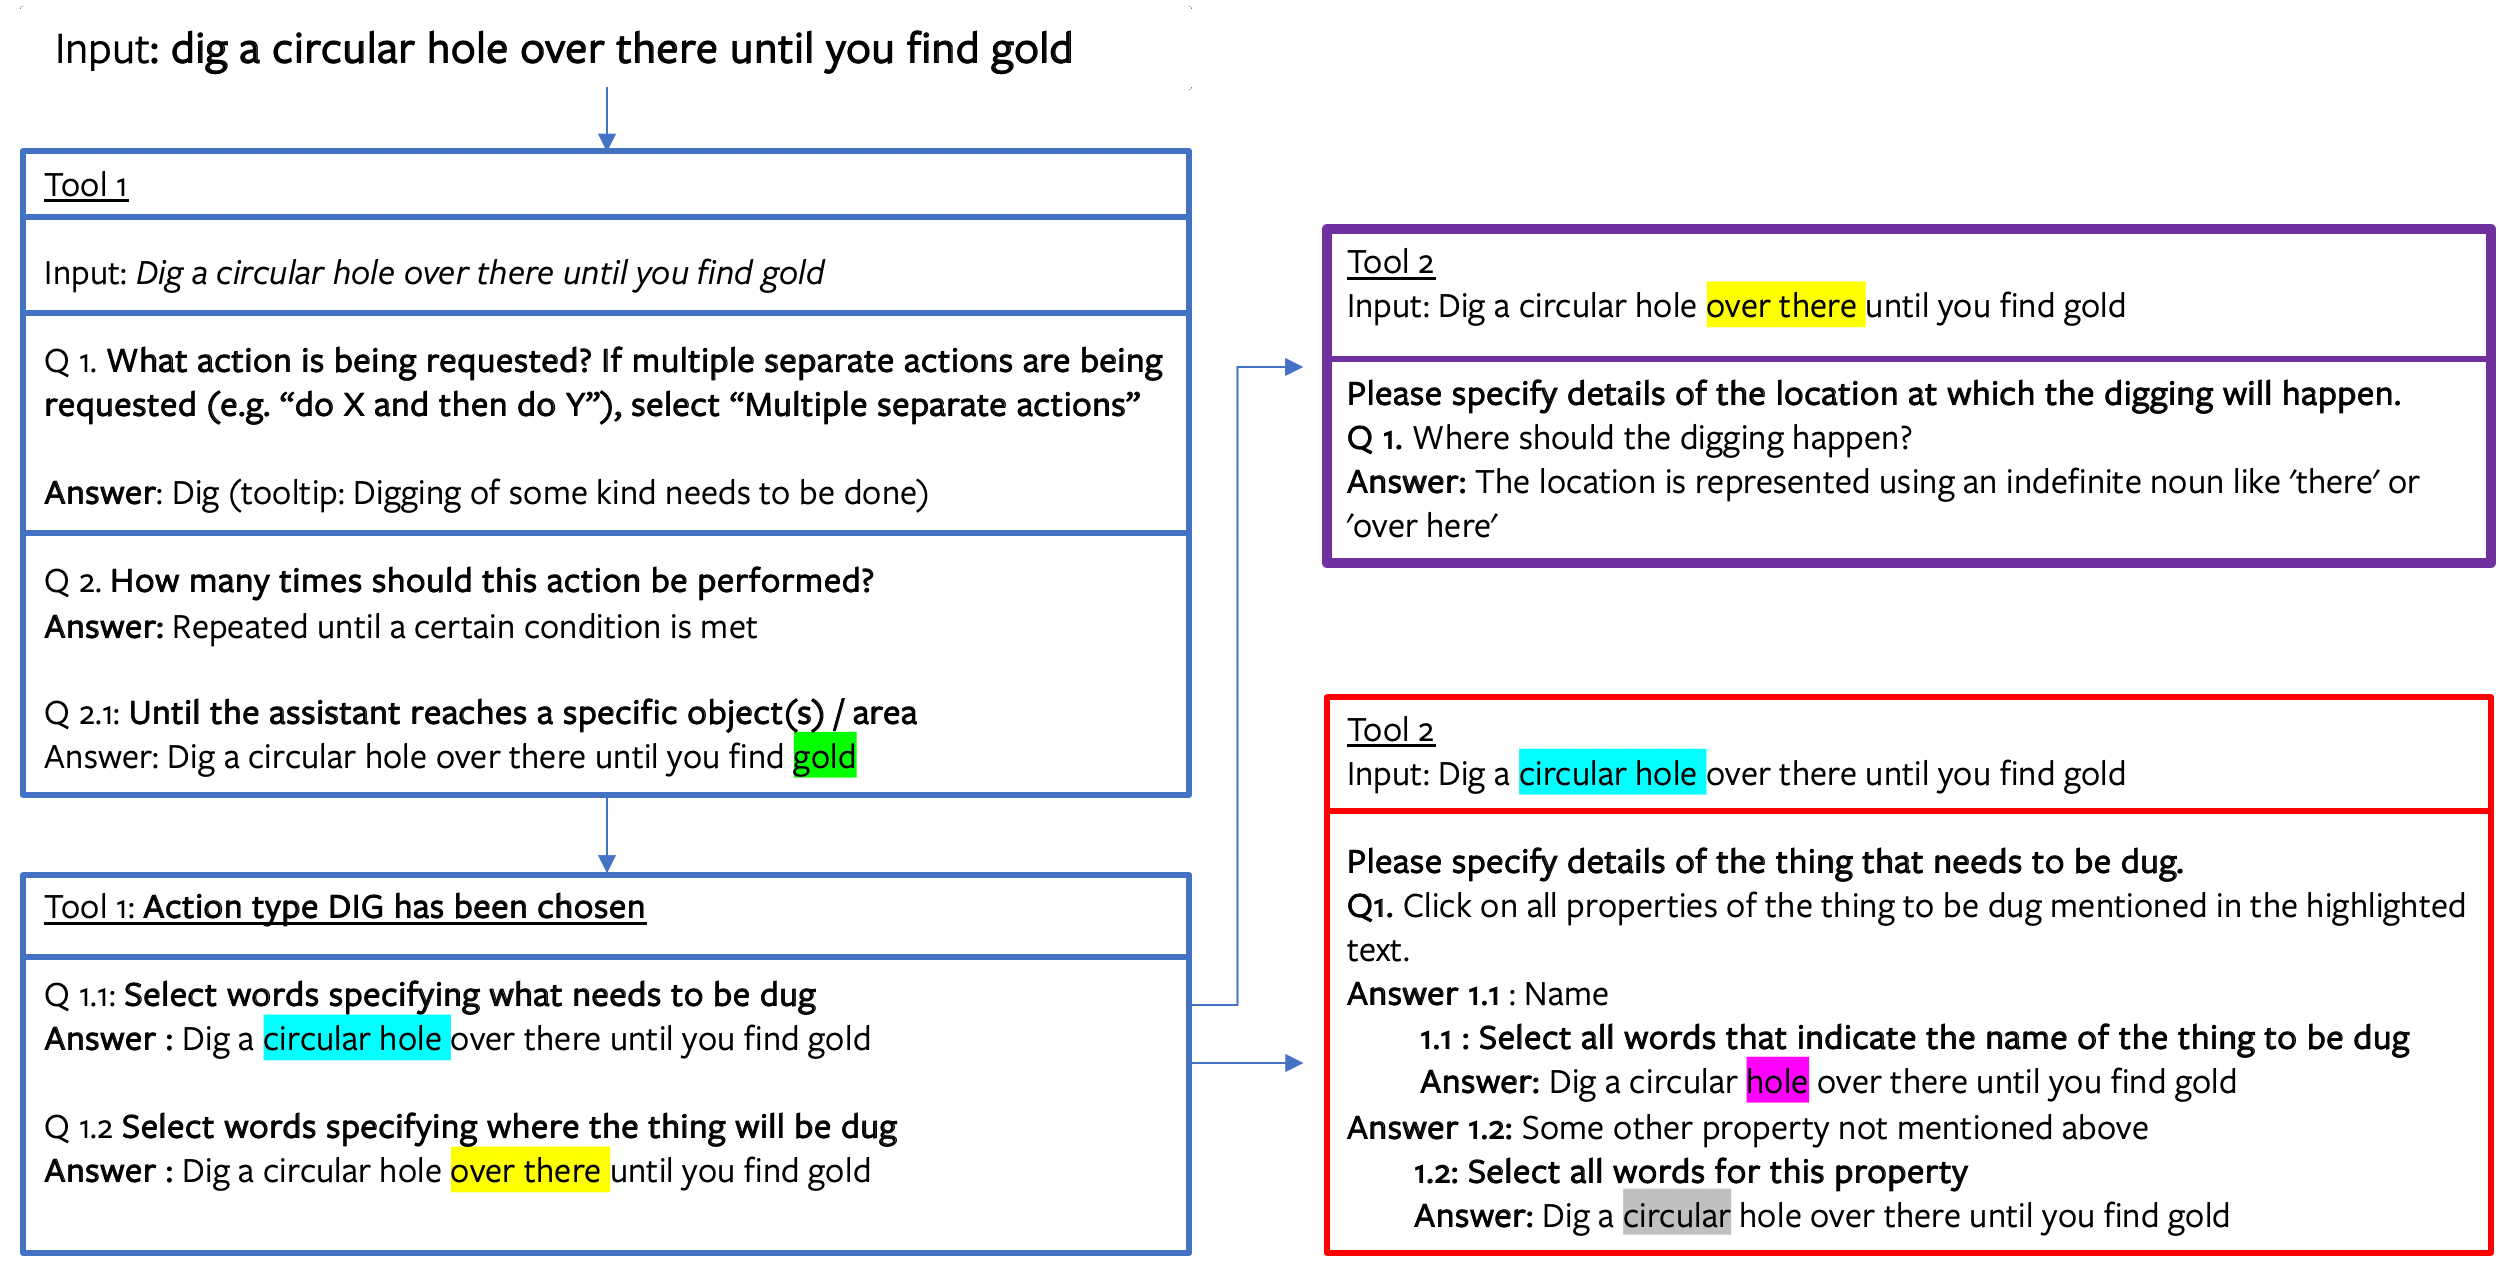
\includegraphics[width=\linewidth, height=6 cm  ]{figures/tools_diagram2.png}
 \caption{A representation of the annotation process using the web-based annotation tool described in Section \ref{sec:annotation}.  The colors of the boxes correspond to annotation tasks.  The highlighting on the text in the header of the later tasks is provided by a previous annotator.  We show more detailed screenshots of how the tool works in Appendix \ref{sec:anntn}}.
\label{fig:tool}
\end{figure*}

\subsection{Logical Forms}
The focus of this paper is an intermediate representation that allows natural language to be interpreted into programs over the basic actions from the previous section. 
The logical forms (represented as trees) making up this representation consist of three basic types of nodes: ``internal nodes'' that can have children, ``categorical'' (leaf) nodes that belong to a fixed set of possibilities, and ``span'' nodes that point to a region of text in the natural language utterance.   The full grammar is shown in the Appendix; and a partial schematic representation is shown in Figures \ref{fig:AS} and \ref{fig:NOT_AS}.  In the paragraphs below, we give more detail about some of the kinds of nodes in the grammar.     

We emphasize that this is an {\it intermediate} representation.   The logical forms do not come with any mechanism for generating language, and nodes do not correspond in any simple way with words.  On the other hand, the logical forms do not encode all of the information necessary for execution without the use of an interpreter that can access the assistant's memory and the Minecraft world state.   

%. Figure~\ref{fig:example_parse} presents an example parse tree for the \textsc{build} command \textit{``Make three oak wood houses to the left of the dark grey church.''}

\smallskip

\noindent{\bf Internal nodes: } Internal nodes are nodes that allow recursion; although most do not require it. 
 They can correspond to top-level actions, for example \textsc{Build}; in which case they would just be an ``action'' node with ``action\_type'' build; 
 see Figure \ref{fig:AS}.  They can also correspond to arguments to top-level actions, for example a ``reference\_object'', which specifies an object that has a spatial location.   
  Internal nodes are not generally required to have children;
   it is the job of the interpreter to deal with under-specified programs like a \textsc{Build} with no arguments. 

%Each action has a set of possible arguments, which themselves have a recursive argument structure. Each of these action types and complex arguments corresponds to an internal node (blue rounded rectangles in Figure~\ref{fig:example_parse}), with its children providing more specific information. For example, the \textsc{build} action can specify a \textsc{schematic} (what we want to build) and a \textsc{location} child (where we want to build it). In turn, the \textsc{schematic} can specify a general category (house, bridge, etc\ldots), as well as a set of properties (size, building material, etc...), and in our case also has a \textsc{repeat} child subtree specifying how many we want to build. Similarly, the \textsc{location} can specify an absolute location, a distance, direction, and information about the location \textsc{reference object} stored in a child subtree.

%One notable feature of this representation is that we do not know \textit{a priori} which of a node's possible children will be specified. For example, \textsc{build} can have a \textsc{schematic} and a \textsc{location} specified (\textit{``Build a house over there.''}), just a \textsc{schematic} (\textit{``Build a house.''}), just a \textsc{location} (\textit{``Build something next to the bridge.''}), or neither (\textit{``Make something.''}).

 In addition to the various \textsc{location}, \textsc{reference object}, \textsc{schematic}, and \textsc{repeat} nodes which can be found at various levels, another notable sub-tree is the action's \textsc{stop condition}, which essentially allows the agent to understand ``while'' loops (for example: ``dig down until you hit the bedrock'' or ``follow me'').  

\smallskip

\noindent{\bf Leaf nodes: } Eventually, arguments have to be specified in terms of values which correspond to (fixed) agent primitives. We call these nodes categorical leaves (green rectangles in Figures \ref{fig:AS} and \ref{fig:NOT_AS}).  As mentioned above, an ``action'' internal node has a categorical leaf child which specifies the \textbf{action type}. There are also \textbf{repeat type} nodes similarly specifying a kind of loop  for example in  the \textsc{repeat} sub-tree corresponding to "make three houses" the \textbf{repeat type} \textbf{for} specifies a ``for'' loop).   There are also \textbf{location type} nodes specifying if a location is determined by a reference object, a set of coordinates, etc.;  \textbf{relative direction} nodes that have values like ``left'' or ``right''. The complete list of categorical nodes is given in the Appendix.

However, there are limits to what we can represent with a pre-specified set of hard-coded primitives, especially if we want our agent to be able to learn new concepts or new values. Additionally, even when there is a pre-specified agent primitive, mapping some parts of the command to a specific value might be better left to an external module (e.g. mapping a number string to an integer value). For these reasons, we also have span leaves (red ovals in Figure~\ref{fig:NOT_AS}). %This way, a model can learn to generalize to e.g. colors or size descriptions that it has never seen before.   
For example, in the parse for the command  \textit{``Make three oak wood houses to the left of the dark grey church.''}, %starting from the ``action'' internal node, is {action: action_type: ``BUILD''
the \textsc{schematic} (an internal node) might be specified by the command sub-string corresponding to its \textbf{name} by the span``houses''  and the requested \textbf{block type} by the span ``oak wood''. The range of the for loop is specified by the \textsc{repeat}'s \textbf{for value} (``three''), and the \textsc{reference object} for the location is denoted in the command by its generic \textbf{name} and specific \textbf{color} with spans ``church'' and ``dark grey''.

 \smallskip

\noindent{\bf The root: } The root of the tree has three productions:   \textsc{put\_memory}, and \textsc{get\_memory}, corresponding to writing to memory and reading from memory; and \textsc{human\_give\_command} which also produces an \textsc{action\_sequence}, which is a special internal node whose children are ordered; multiple children correspond to an ordered  sequence of commands (``build a house and then a tower'').  In Figures \ref{fig:AS} and \ref{fig:NOT_AS} we show a schematic representation for an \textsc{action\_sequence}.
\section{The CAIP Dataset}
\label{sec:data}

This paper introduces the CraftAssist Instruction Parsing (CAIP) dataset of English-language commands and their associated logical forms (see Appendix~\ref{sec:action_tree} for examples and a full grammar specification).  
\begin{comment}
The  number of examples of each kind as well as the training/test split are presented in Table~\ref{tab:dataset_stats}.

\begin{table}[t!]
\center
\begin{tabular}{l|ccc}
Split       & Train   	& Val    & Test \\
\midrule % & Total  \\ \hline
%Templated   & 510K  	& 5K     & 5K   \\ % & 4     \\
%Rephrases   & 27K     	& 2K     & 2370  \\ % & 8     \\
Prompts     & -       	& 1500   & 3032 \\ %  & 12    \\
Interactive & -       	& 661    & 1500  \\ %  & 16    \\ \hline
\end{tabular}
\caption{Data splits for all data collection processes. \label{tab:dataset_stats}}
\end{table}



\subsection{Templated Data}
\label{sec:generated_data}

We algorithmically generate logical forms over the grammar with associated surface forms through the use of templates. To that end, we first define a set of {\it template objects}.  These might  link a concept in the game world to several ways it can be described through language.  For example the template object \texttt{Move} links the action type \textsc{move} to the utterances \textit{go},  \textit{walk},  \textit{move},\ldots 
%Likewise, the template object \texttt{RelativeDirection} links all of the assistant's direction primitives to their names. 
 Other template objects have purely decorative functions (w.r.t. the assistant's action space), for example \texttt{Please}.
 %and are in order to make the sentence more natural. For example, the object \texttt{ALittle} can be realized into \textit{a bit},  \textit{a little}, \textit{somewhat}, \ldots . 
 The set of possible realizations for each template object is manually defined.

Then, we build {\it templates} for each action as recursive sequences of templates and template objects. For each of these templates, we can then sample a game value and its corresponding string. By concatenating these, we obtain a logical form and its corresponding language description. Consider for example the template [\texttt{Move}, \texttt{ALittle}, \texttt{RelativeDirection}].% made up of the template objects described above. 
One possible realization could be the description \textit{go a little to the left} paired with a logical form specifying the action type as \textsc{move}, and an \textsc{action location} sub-tree with which a child relative direction categorical node which has value \textsc{left}. 

%We handle compositionality by combining different action templates together in order, for example to generate: \textit{go there and build me a big circle}  we combined respective templates from \textsc{move} action and \textsc{build} action to give an ordered sequence of actions under ``action\_sequence'' in the tree. 

We generate
training data for the \textsc{noop} action type by sampling dialogue lines from the Cornell Movie Dataset \cite{Danescu-Niculescu-Mizil+Lee:11a}.


We wrote 3,900 templates in total. We can create a training example for a parsing model by choosing a template at random, and then sampling a (description, tree) pair from it, which, given the variety and modularity of the template objects, yields virtually unlimited data (for practical reasons, we pre-generate a set of 510K training, 5K validation, and 5K test examples for our experiments). The full list of templates and template objects is included in the Supplementary Material.

% We generated a large database of natural language commands and their corresponding action trees using a system of hierarchically composable templates. Each action is characterized by a set of supported templates, each of which is an ordered list of template objects.

% To generate a command, we choose a random action from the set of supported actions (a complete list is presented in section \ref{sec:action_tree}) and then a random template is chosen from the action's template set. Each template object is then converted to text to produce the command, and key-value pairs to produce the action tree.

% An example template for the \textsc{Move} action is composed of the  objects. Given different resolutions of each object, the template might produce commands like "move a little to the right" or "can you walk a bit south". Some template objects affect the action tree (e.g. the "relative\_direction" key is different in the two examples above), while others like \texttt{ALittle} do not.

% Template objects may also make use of other template objects, making the conversion to text a recursive process. The text and action tree fragments produced by template objects that are shared across templates can be reused (e.g. both the \textsc{Move} and \textsc{Build} actions may specify a \texttt{Location}).

\end{comment}




\begin{figure}
\center
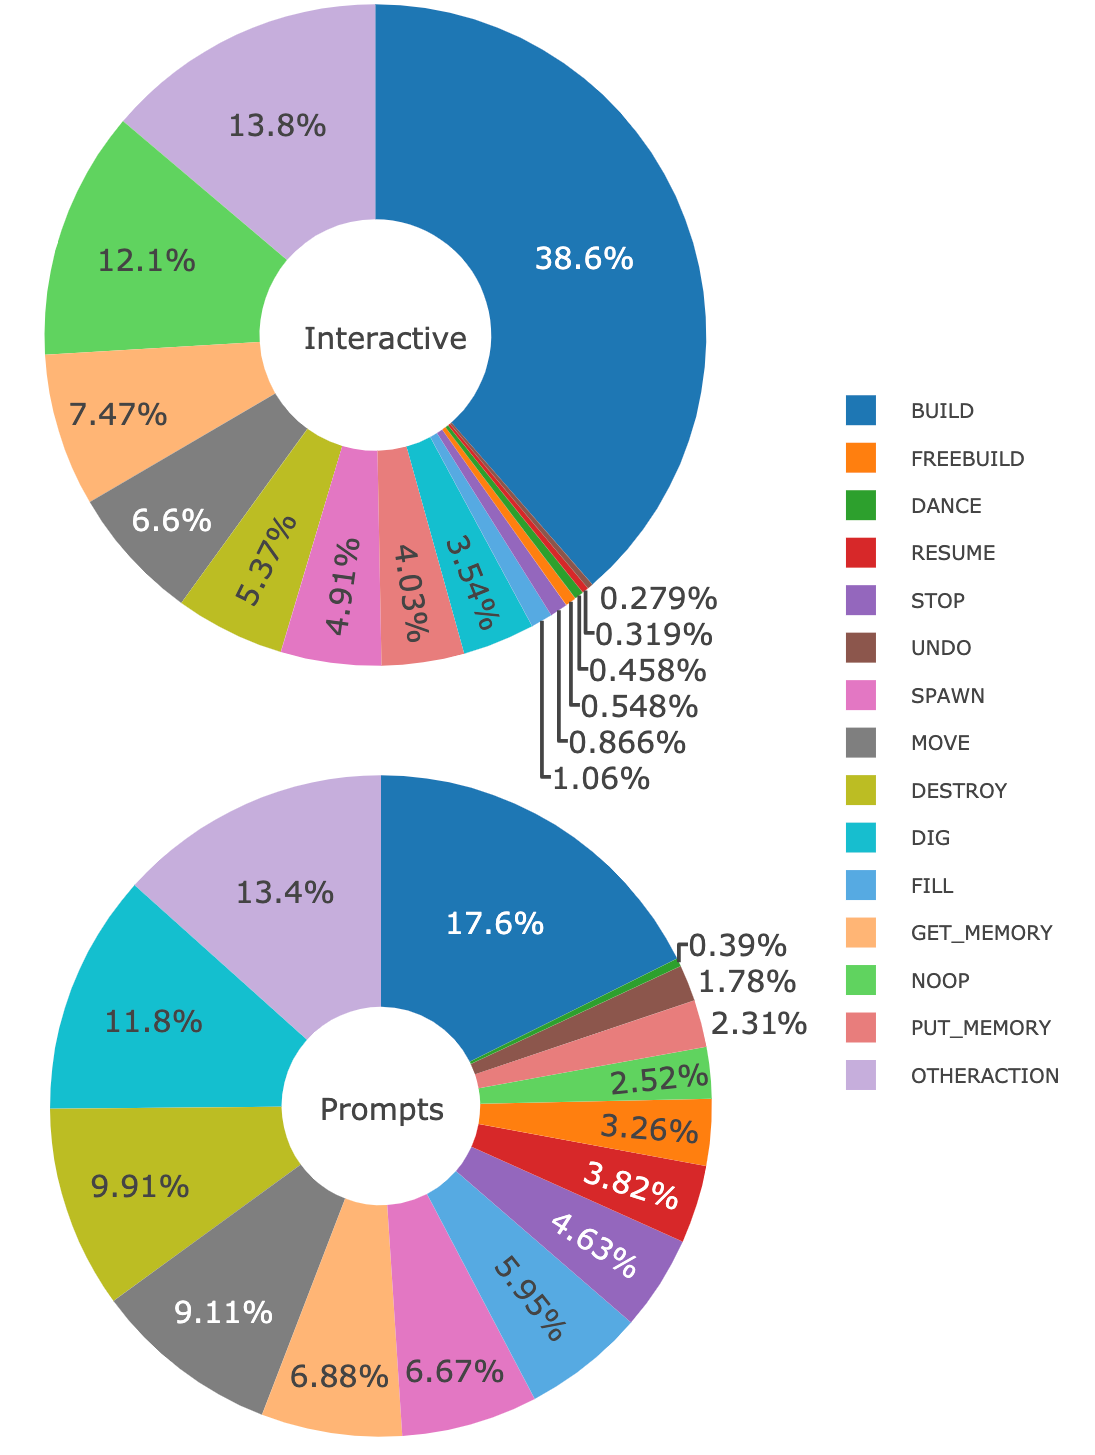
\includegraphics[width=0.9\linewidth ]{figures/action_freq2_vert.png}
\caption{Frequency of each action type in the different data collection schemes described in Section~\ref{sec:collected_data}.
\label{fig:action_freqs}
}
\end{figure}

\subsection{Collected Data}
\label{sec:collected_data}

%To supplement the generated data, 
We collected natural language commands written by crowd-sourced workers  in a variety of settings. The complete list of instructions given to crowd-workers in different settings, as well as step-by-step screen-shot of the annotation tool, are provided in the Appendix \ref{sec:instructions}.  The basic data cleanup is described in Appendix \ref{sec:data_cleanup}.

\begin{figure}
\center
%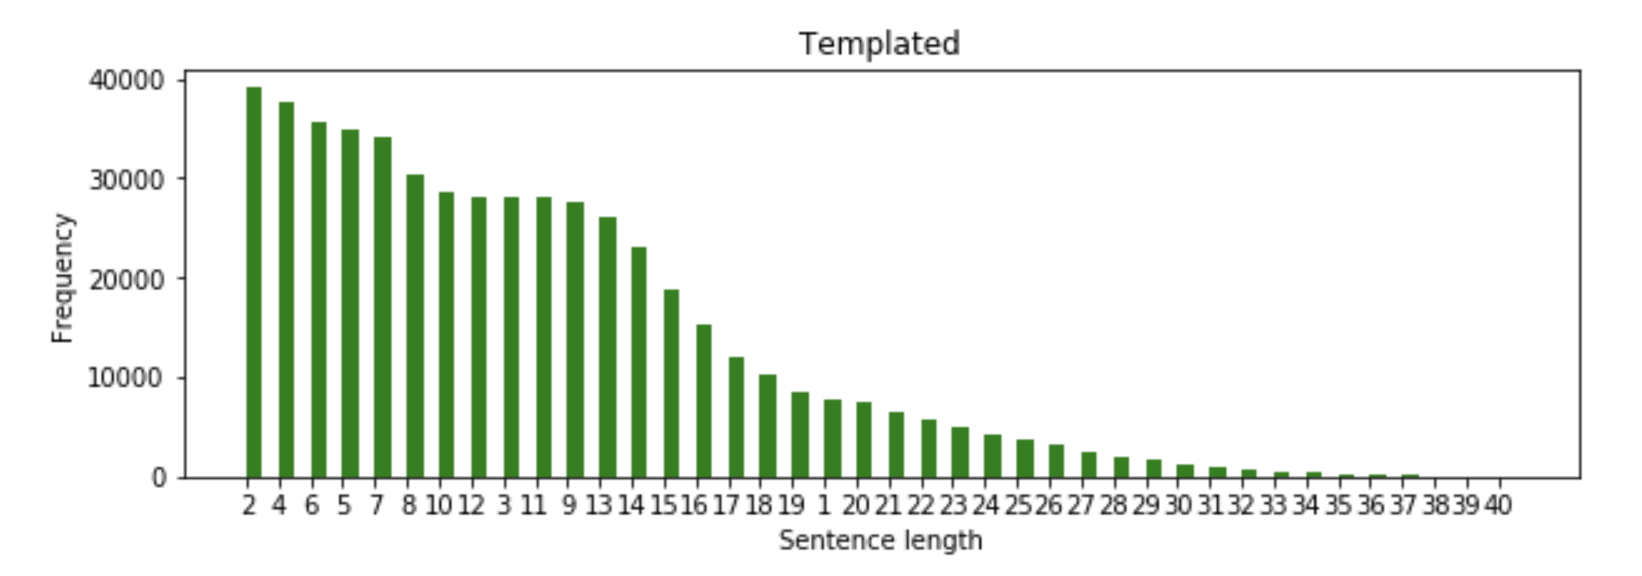
\includegraphics[width=0.3\linewidth ]{figures/sent_len_temp.png}
\hspace*{-.2cm}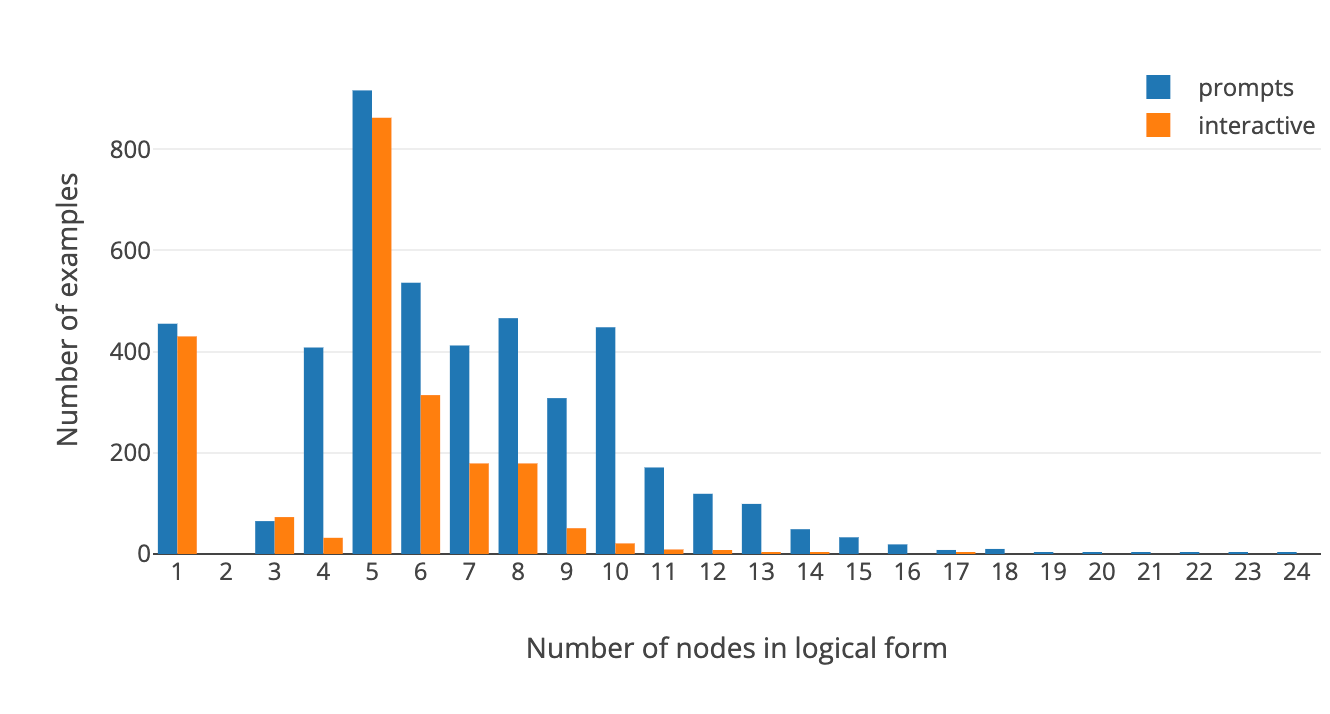
\includegraphics[width=1\linewidth, height=0.35\linewidth]{figures/nodenum_histogram}
\hspace*{-.2cm}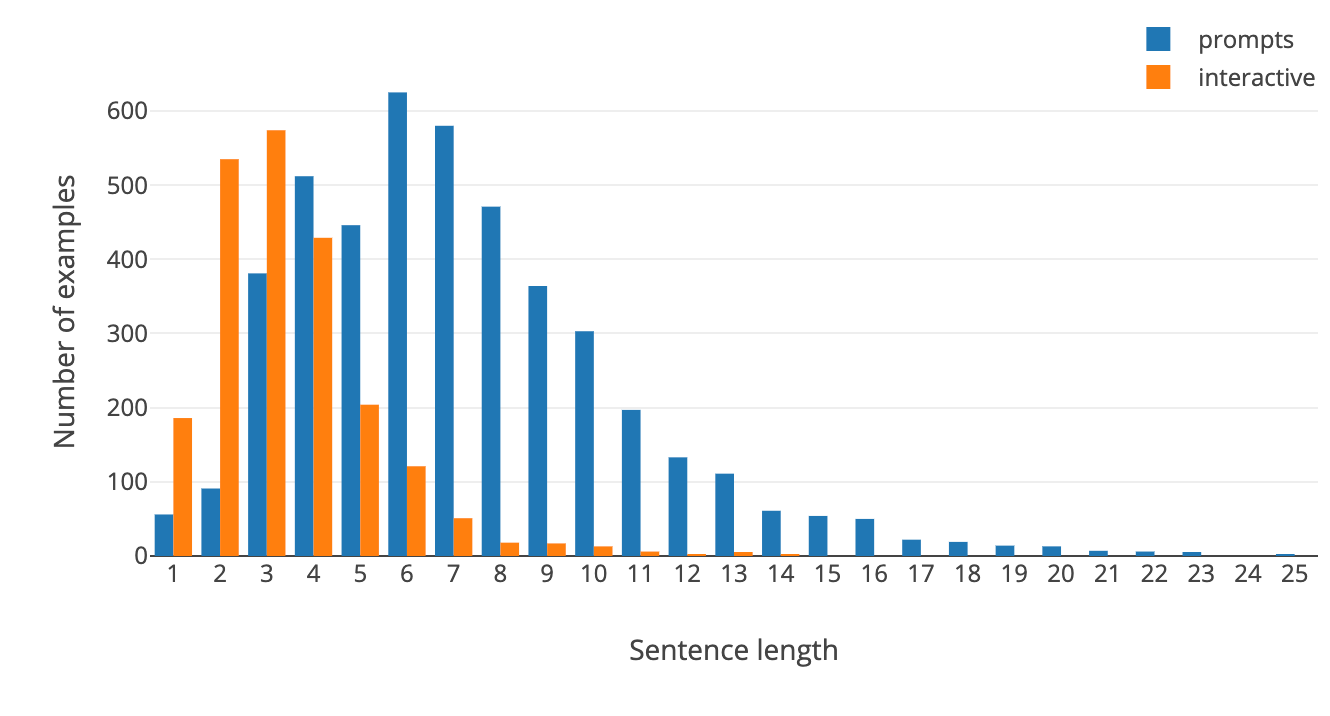
\includegraphics[width=1\linewidth, height=0.35\linewidth]{figures/sentence_length_histogram}
\caption{Histograms showing distribution over number of nodes in a logical form (top) and utterance length in words (bottom) for each data type. Prompts averages 6.74 nodes per logical form, 7.32 words per utterance, and interactive averages 4.89, 3.42 respectively}
\label{fig:quant_sent_len}
\end{figure}



%\subsubsection{Rephrases} While the template generations yield a great variety of language, they cannot cover all possible ways of phrasing a specific instruction. In order to supplement them, we asked crowd-sourced workers to  rephrase some of the produced instructions into commands in alternate, natural English that does not change the meaning of the sentence. This setup enables the collection of unique English commands whose action trees are already known. Note that a rephrased sentence will have the same action tree structure, but the positions of the words corresponding to span nodes may change. % , and hence the values of the spans.
% For example, the command "build a pillar", represented by the action tree:  \{"Build": \{"schematic": \{"has\_name\_": [2,~2]\}\}\}, might be rephrased to "make me a pillar", where the word "pillar" has now moved to index 3. 
%To account for this, words contained in a span range in the original sentence are highlighted in the task, and crowd-sourced workers are asked to highlight the corresponding words in their rephrased sentence. Then the action tree span values are substituted for the rephrased sentence to get the corresponding tree. This yields a total of 32K rephrases.
%We selected the instructions to be rephrased at random and assessed the quality of rephrases by throwing away all mistakes made by humans when highlighting the spans. If the any spans were missing or the highlighting wasn't done properly, we threw the rephrase data away.
% We use 30K for training, 1K for validation, and 1K for testing.


\subsubsection{Image and Text Prompts} \label{sec:prompts}We presented crowd-sourced workers with a description of the capabilities of an assistant bot in a creative virtual environment (which matches the set of allowed actions in the grammar), and (optionally) some images of a bot in a game environment. They were then asked to provide examples of commands that they might issue to an in-game assistant. We refer to these instructions as ``prompts'' in the rest of this paper.
% The complete instructions shown to workers is included in appendix \ref{fig:freegen}.

% The process of annotating these sentences with their corresponding action trees is described in section \ref{sec:annotation_tool}.

\subsubsection{Interactive Gameplay}\label{sec:human_bot} We asked crowd-workers to play creative-mode Minecraft with our assistant bot, and they were instructed to use the in-game chat to direct the bot as they chose. The game sessions were capped at 10 minutes and players in this setting had no prior knowledge of the bot's capabilities or the grammar. We refer to these instructions as ``Interactive'' in the rest of this paper.
The instructions of this setting are included in Appendix \ref{sec:appen}. 
% Each line of in-game chat written by a player in this scenario was annotated with its corresponding action tree by the process described in section \ref{sec:annotation_tool}.

% \subsubsection{Annotation tool}
% \label{sec:annotation_tool}



\subsubsection{Annotation Tool}
\label{sec:annotation}

Both prompts and interactive instructions come without a reference logical form and need to be annotated. To facilitate this process,
% the annotation of a natural language command with its corresponding action tree representation,
 we designed a multi-step web-based tool which asks users a series of multiple-choice questions to determine the semantic content of a sentence. The responses to some questions will prompt other more specific questions, in a process that mirrors the hierarchical structure of the grammar. The responses are then processed to produce the complete logical form.
This allows crowd-workers to provide annotations with no knowledge of the specifics of the grammar described above. A pictorial representation of the annotation process is shown in Figure \ref{fig:tool} and a more detailed explanation of the process along with screen-shots of the tool is given in Appendix  \ref{sec:anntn}.

%As a first step of the execution, we had crowd-workers annotate three different sentences that were representative  of our grammar and we assigned them qualification scores. Workers who scored a 100\% accuracy on these, made it to our ``qualified'' workers pool and helped us annotate the entire dataset. 
We used a small set of tasks that were representative of the actual annotations to select skilled crowd-sourced workers by manually verifying the accuracy of responses on these.

Each utterance in our collection of prompts and interactive  chats was shown to three different qualified annotators and we included the utterance and logical form in the dataset only if at least 2 out of 3 qualified annotators agreed on the logical form output.   The total number of utterances sent to turkers was 6,775.  Out of these, 6,693 had at least 2/3 agreements on the logical form and were kept.  Of these, 2,872 had 3/3 agreements. 


The final dataset has  4,532 annotated instructions from the prompts setting (Section~\ref{sec:prompts}), and 2,161 from interactive play (Section~\ref{sec:human_bot}). The exact instructions shown to Turkers in the annotation tools are reproduced in Figures \ref{fig:annotation_task1} and \ref{fig:annotation_task2} in supplementary.
% A screenshot of the tool is included in Appendix \ref{fig:annotation_task}.
 
As in \citep{yih2016value}, we have found that careful design of the annotation tool leads to significant improvements in efficiency and accuracy.  In particular, we re-affirm the conclusion from \cite{yih2016value} that having each worker do one task (e.g. labeling a single node in the tree) makes annotation easier for workers. %Along with good annotation accuracy, we also got the annotations quickly (about 1500 annotations in just two hours).
\begin{comment}
\begin{table}
\center
\begin{tabular}{l|cc}
Split       & Avg sent length   	& Avg no of nodes\\
\midrule % & Total  \\ \hline
%Templated   & 10.06  	& 9.63     \\ % & 4     \\
%Rephrases   & 9.01     	& 8.34      \\ % & 8     \\
Prompts     & 7.32       	& 6.74      \\ %  & 12    \\
Interactive & 3.42       	& 4.89      \\ %  & 16    \\ \hline
\end{tabular}
\caption{Average sentence length and average number of nodes in the tree per data split. \label{tab:sent_len}}
\end{table}
\end{comment}
\subsection{Dataset Statistics}
\label{sec:dataset_statistics}

\subsubsection{Action Frequencies}
Since the different data collection settings described in Section~\ref{sec:collected_data} imposed different constraints and biases on the crowd-sourced workers, the distribution of actions in each subset of data is therefore different. 
%For example, in the Interactive Gameplay scenario, workers were given no prior indication of the bot's capabilities, and spent much of their time asking the bot to build things. 
The action frequencies of each subset are shown in Figure~\ref{fig:action_freqs}.


\subsubsection{Grammar coverage} 
Some crowd-sourced commands describe an action that is outside the scope of the grammar. To account for this, users of the annotation tool are able to mark that a sentence is a command to perform an action that is not covered by our grammar yet. The resulting trees are labeled as \textsc{OtherAction}, and their frequency in each dataset in shown in Figure~\ref{fig:action_freqs}. Annotators still have the option to label other nodes in the tree, such as the action's \textsc{location} or \textsc{reference object}.  In both the prompts and interactive data, \textsc{OtherAction} amounted to approximately $14\%$ of the data.
%Some crowd-sourced commands describe an action that is outside the scope of the grammar. Humans also sometimes ask a bot to execute several actions in one command. To account for this, users of the annotation tool are able to mark that a sentence is a command to perform a composite action or an action that is not covered by our grammar yet. The resulting trees are labeled as \textsc{composite} and \textsc{OtherAction} respectively, and their frequency in each dataset in shown in Figure~\ref{fig:action_freqs}. Note that annotators that choose either still have the option to label other nodes in the tree, such as the action's \textsc{location} or \textsc{reference object}.


\subsubsection{Quantitative analysis} 
\label{sec:quant_analysis}
For each of our data types, Figure \ref{fig:quant_sent_len}  show a histogram of sentence length and number of nodes.   On an average interactive data has shorter sentences and smaller trees.
%On an average, templated data has longer sentences and deeper action trees followed by prompts and then interactive data. 

\subsubsection{Qualitative Linguistic Style} We show the linguistic styles and choice of words of the data sources by displaying the surface forms of a set of trees. We randomly picked trees of size (number of nodes) 7 that appear in both data sources, and then for the same tree structure, we looked at the utterances corresponding to that tree. We show some representative examples in table \ref{tab:ling_1}.  We show more examples of the data in the Appendix.


\begin{table*}
\center
\small
%\begin{tabular}{c p{1.9cm} p{4.2cm} p{3.2cm}}
%Templated   & go to tree  	& please make very large cave     & install sphere here      \\  \hline% & 4     \\
%%Rephrases   & 27K     	& 2K     & 2370  \\ % & 8     \\
%Prompts     &bot move to \mbox{where the tree is}       	& dig a large size hole to put these waste particles into the hole   & please build a sphere on that location      \\  \hline%  & 12    \\
%Interactive & find tree       	& dig large hole    & build a sphere over here   \\ \hline %  & 16    \\ \hline
%\end{tabular}
\begin{tabular}{r  m{2.0cm} m{4.2cm} m{3.0cm} m{3.0cm}}
\toprule
%Templated:   &  go to tree  	& please make very large cave     & install sphere here     & build hole five tiles long 5 blocks wide   \\  
%\midrule% & 4     \\
%Rephrases   & 27K     	& 2K     & 2370  \\ % & 8     \\
Prompts     & bot move to \mbox{where the tree is}& dig a large size hole to put these waste particles into the hole   & please build a sphere on that location       	& hey bot can you dig a 5 by 5 hole for me   \\  \midrule%  & 12    \\
Interactive & find tree       	& dig large hole    & build a sphere over here    & dig a 5 x 5 hole  \\ \bottomrule %  & 16    \\ \hline
\end{tabular}
\caption{Choice of words across different data sources for the same logical form (per column).}
\label{tab:ling_1}
\end{table*}


%In addition to above, we also looked at precision, recall and f1 scores of n-grams of prompts and interactive data with templated and have reported the  numbers for unigram, bi-gram, tri-gram and four-grams in table \ref{tab:N-gram}Conclusion of this here ?

%Rephrases: assist me to clear a large mine





\section{Related Work}

%Semantic parsing -- 1970s AI -- Question answering approaches -- FSP -- Grounded Language -- Relevant MC recent work -- Alexa Meaning Representation / Challenge


There have been a number of datasets of natural language paired with logical forms to evaluate semantic parsing approaches, e.g. \cite{price1990evaluation, tang2001using, cai2013large, wang2015building, zhong2017seq2sql}. The dataset presented in this work is an order of magnitude larger than those in \cite{price1990evaluation, tang2001using, cai2013large} and is similar in scale to the datasets in \cite{wang2015building}, but smaller than \cite{zhong2017seq2sql}. 
%We use a similar data collection strategy to \cite{wang2015building}: first define the grammar of possible semantic parses, then use it to generate parse trees along with corresponding text description via templates, and finally ask crowd-sourced workers to rephrase the templated generations into more natural language. We also collect a set of ``free'' commands and use crowd-sourced workers to annotate these.


In addition to mapping natural language to logical forms, our dataset connects both of these to a dynamic environment.  
In \cite{lauria2001training, bos2007spoken, tellex2011understanding, matuszek2013learning, thomason2019improving} semantic parsing has been used for interpreting natural language commands for robots. %, matuszek2013learning}.  
In our paper, the ``robot'' is embodied in the Minecraft game instead of in the physical world. In \cite{Boye2006RobustSL} semantic parsing has been used for spoken dialogue with an embodied character in a 3-D world with pattern matching and rewriting phases. In our work, the user along with the assistant is embodied in game and instructs using language. We go from language to logical forms end-to-end with no pattern match necessary.
%\cite{matuszek2013learning} :~500 examples, RCL differences (but similar- we have loops etc.), deep models instead of feature reps, templates
%
Semantic parsing in a voxel-world recalls \cite{wang2017naturalizing}, where the authors describe a method for building up a programming language from a small core via interactions with players.  %In this work, we made a substantial effort to build coverage ourselves via a corpus of templates, but 

%\cite{wang2016learning, wang2017naturalizing} %maybe second cite should go to discussion
 

We demonstrate the results of several neural parsing models on our dataset.  In particular, we show the results of a re-implementation of \cite{dong2016language} adapted to our grammar, and a straightforward fine-tuned BERT model \cite{devlin2018bert}. There have been several other papers proposing neural architectures for semantic parsing, for example \cite{jia2016data, zhong2017seq2sql, wang2018transfer, hwang2019comprehensive}; in particular \cite{hwang2019comprehensive} uses a BERT based model.  In those papers, as in this one, the models are trained with full supervision of the mapping from natural language to logical forms, without considering the results of executing the logical form (in this case, the effect on the environment of executing the actions denoted by the logical form). There has been progress towards ``weakly supervised'' semantic parsing
% (with or without deep architectures ) 
 \cite{artzi2013weakly, liang2016neural, guu2017language} where the logical forms are hidden variables, and the only supervision given is the result of executing the logical form. There are now approaches that have shown promise without even passing through (discrete) logical forms at all \cite{riedel2016programming, neelakantan2016learning}.  We hope that the dataset introduced here, which has supervision at the level of the logical forms, but whose underlying grammar and environment can be used to generate essentially infinite weakly supervised or execution rewards, will also be useful for studying these models.


Minecraft, especially via the MALMO project \cite{johnson2016malmo} has been used as a base environment for several machine learning papers. It is often used as a testbed for reinforcement learning (RL) \cite{shu2017hierarchical,udagawa2016fighting,alaniz2018deep,oh2016control,tessler2017deep}. In these works, the agent is trained to complete tasks by issuing low level actions (as opposed to our higher level primitives) and receiving a reward on success.  Others have collected large-scale datasets for RL and imitation learning \cite{guss2019minerlCompetition, guss2019minerl}.   Some of these works (e.g. \cite{oh2017zero}) do consider simplified, templated language as a method for composably specifying tasks, but training an RL agent to execute the scripted primitives in our grammar is already nontrivial, and so the task space and language in those works is more constrained  than what we use here.  Nevertheless, our work may be useful to researchers interested in RL (or imitation): using our grammar and executing in game can supply (hard) tasks and descriptions, and demonstrations.
Another set of works \cite{kitaev2017misty, yi2018neural} have used Minecraft for visual question answering with logical forms. Our work extends these to interactions with the environment.
Finally, \cite{allison2018players} is a more focused study on how a human might interact with a Minecraft agent; our collection of free generations (see \ref{sec:prompts}) includes annotated 
examples from similar studies of players interacting with a player pretending to be a bot.


\section{Baseline Models}
\label{sec:modeling}

In order to assess the challenges of the dataset, we implement two models which learn to read a sentence and output a logical form by formulating the problem as a sequence-to-tree and a sequence-to-sequence prediction task respectively.

\subsection{Sequence to Tree Model}

Our first model adapts the Seq2Tree approach of \citep{dong2016language} to our grammar. In short, a bidirectional RNN encodes the input sentence into a sequence of vectors, and a decoder recursively predicts the tree representation of the logical form, starting at the root and predicting all of the children of each node based on its parent and left siblings and input representation.

\paragraph{Sentence Encoder and Attention: } We use a bidirectional GRU encoder \citep{ChoMGBBSB14} which encodes a sentence of length $T$  $\mathbf{s} = (w_1, \ldots \ w_{T})$ into a sequence of $T$ dimension $d$ vectors:
\begin{equation*}
f_{GRU}(\textbf{s}) = (\mathbf{h}_1,\ldots, \mathbf{h}_T) \in \mathbb{R}^{d \times T}
\end{equation*}
\begin{comment}
The tree decoder is then conditioned on the sequence encoder output via an attention mechanism.
We follow the attention implementation of \cite{opennmt}. Given $K$ matrices $\textbf{M}^\alpha = (M_1^\alpha,\ldots, M_1^\alpha) \in \mathbb{R}^{d \times d \times K}$, we have:
\begin{align*}
& \alpha^k_n = \text{softmax}\Big(\frac{\mathbf{x}^{\text{T}} M^{\alpha}_k (\mathbf{h}_1,\ldots, \mathbf{h}_T)}{\sqrt{d}} \Big) \\
& \mathbf{x}^{\alpha} = \sum_{k=1}^K {\alpha^k_n}^{\text{T}} (\mathbf{h}_1,\ldots, \mathbf{h}_T) \\
& \text{attn}(\mathbf{x}, (\mathbf{h}_1,\ldots, \mathbf{h}_T); \textbf{M}^\alpha) = \mathbf{x} + \mathbf{x}^{\alpha}
\end{align*}
\end{comment}
\paragraph{Tree Decoder: } The decoder starts at the root, computes its node representation and predicts the state of its children, then recursively computes the representations of the predicted descendants. Similarly to Seq2Tree, a node representation $\mathbf{r}_n$ is computed based on its ancestors and left siblings. We also found it useful to condition each of the node representation on the encoder output explicitly for each node. Thus, we compute the representation $\mathbf{r}_{n_t}$ and recurrent hidden state $\mathbf{g}_{n_t}$ for node $n_t$ as:
\begin{align}
& \mathbf{r}_{n_t} = \text{attn}(\mathbf{v}_{n_t} + \mathbf{g}_{n_{t-1}}, (\mathbf{h}_1,\ldots, \mathbf{h}_T); \; \textbf{M}^\sigma) \\
& \mathbf{g}_{n_{t}} =
    f_{rec}(\mathbf{g}_{n_{t-1}}, (\mathbf{v'}_{n_t} + \mathbf{r}_{n_t}))
\end{align}
Where  $\text{attn}$ is multi-head attention, $\textbf{M}^{\sigma} \in \mathbb{R}^{d \times d \times K}$ is a tree-wise parameter, $f_{rec}$ is the GRU recurrence function, and $\mathbf{v'}_{n_t}$ is a node parameter (one per category for categorical nodes), and $n_{t-1}$ denotes either the last predicted left sibling if there is one or the parent node otherwise.

\paragraph{Prediction Heads: } Finally, the decoder uses the computed node representations to predict the state of each of the internal, categorical, and span nodes in the grammar. We denote each of these sets by $\mathcal{I}$, $\mathcal{C}$ and $\mathcal{S}$ respectively, and the full set of nodes as $\mathcal{N} = \mathcal{I} \cup \mathcal{C} \cup \mathcal{S}$.

First, each node in $\mathcal{N}$ is either active or inactive in a specific logical form. We denote the state of a node $n$ by ${a_n \in \{0, 1\}}$. All the descendants of an inactive internal node $n \in \mathcal{I}$ are considered to be inactive. Additionally, each categorical node $n \in \mathcal{C}$ has a set of possible values $C^n$; its value in a specific logical form is denoted by the category label ${c_n \in \{1,\ldots,|C^n|\}}$. Finally, active span nodes $n \in \mathcal{S}$ for a sentence of length $T$ have a start and end index ${(s_n, e_n) \in \{1,\ldots,T\}^2}$. We compute, the representations $\mathbf{r}_n$ of the nodes as outlined above, then obtain the probabilities of each of the labels by:
\begin{align}
&\forall n \in \mathcal{N}, &p(a_n) &= \sigma(\langle \mathbf{r}_n, \mathbf{p}_n \rangle) \label{eq:int_pred}\\
&\forall n \in \mathcal{C}, &p(c_n) &= \text{softmax}(M^c_n \mathbf{r}_n) \label{eq:cat_pred} \\
&\forall n \in \mathcal{S}, &p(s_n) &= \text{softmax}(\mathbf{r}_n ^{\text{T}} M^s_n (\mathbf{h}_1,\ldots, \mathbf{h}_T)) \nonumber \\
& &p(e_n) &= \text{softmax}(\mathbf{r}_n ^{\text{T}} M^e_n (\mathbf{h}_1,\ldots, \mathbf{h}_T)) \label{eq:span_pred}
\end{align}
where the following are model parameters:
\begin{align*}
\forall n \in \mathcal{N},& \quad \mathbf{p}_n \in \mathbb{R}^d\\
\forall n \in \mathcal{C},& \quad M^c_n \in \mathbb{R}^{d \times d} \\
\forall n \in \mathcal{S},& \quad (M^s_n, M^e_n) _n \in \mathbb{R}^{d \times d \times 2}
\end{align*}
Let us note the parent of a node $n$ as $\pi(n)$. Given Equations~\ref{eq:int_pred} to \ref{eq:span_pred}, the log-likelihood of a tree with states $(\textbf{a}, \textbf{c}, \textbf{s}, \textbf{e})$ given a sentence $\textbf{s}$ is then:
\begin{align}
\mathcal{L} & = \sum_{n \in \mathcal{N}} a_{\pi(n)} \log(p(a_n))  + \sum_{n \in \mathcal{C}} a_n \log(p(c_n)) \nonumber \\
& \quad + \sum_{n \in \mathcal{S}} a_n \Big(\log(p(s_n)) + \log(p(e_n))\Big)
\end{align}

Overall, our implementation differs from the original Seq2Tree in three ways,  which we found lead to better performance in our setting. First, we replace single-head with multi-head attention. Secondly, the cross-attention between the decoder and attention is conditioned on both the node embedding and previous recurrent state. Finally, we replace the categorical prediction of the next node by a binary prediction problem: since we know which nodes are eligible as the children of a specific node (see Figures~\ref{fig:AS} and ~\ref{fig:NOT_AS}), we find that this enforces a stronger prior. We refer to this modified implementation as SentenceRec.% in the rest of the paper.

\subsection{Sequence to Sequence Model}

Our second approach treats the problem of predicting the logical form as a general sequence-to-sequence (Seq2Seq) task; such approaches have been used in semantic parsing in e.g. \citep{jia2016data, wang2018transfer}. We take the approach of \citep{jia2016data} and linearize the output trees:
the target sequence corresponds to a Depth First Search walk through the tree representation of the logical form. More specifically the model needs to predict, in DFS order, a sequence of tokens corresponding to opening and closing internal nodes, categorical leaves and their value, and span leaves with start and end sequences.  
\begin{comment}
\begin{itemize}
\item opening of internal nodes, the corresponding sub-tree, then closing the node: \\ \textsc{open:location}, \ldots, \textsc{close:location}
\item categorical leaves along with their value: \\
\textsc{relative\_dir:up} or \textsc{action\_type:build}
\item span leaves, with start and end indexes:\\
\textsc{has\_size}-(1, 2) $\leftarrow$ \emph{make} {\bf{very large}} \emph{doors}
\end{itemize}
\end{comment}
In practice, we let the model predict span nodes in two steps: first predict the presence of the node, then predict the span value, using the same prediction heads as for the SentenceRec model (see Equation~\ref{eq:span_pred} above). With this formalism, the logical form for e.g. {\emph{``build a large blue dome on top of the walls''}} will be:

\begin{footnotesize}
\begin{verbatim}
(ACTION_TYPE:BUILD, OPEN:SCHEMATIC,
   HAS_SIZE, SIZE_SPAN-(2,2),
   HAS_COLOR, COLOR_SPAN-(3,3),
   HAS_NAME, NAME_SPAN-(4,4),
 CLOSE:SCHEMATIC, OPEN:LOCATION,
   LOC_TYPE:REF_OBJECT, REL_DIR:UP,
   OPEN:REF_OBJECT,
     HAS_NAME, NAME_SPAN-(9,9),
   CLOSE:REF_OBJECT,
 CLOSE:LOCATION)
\end{verbatim}
\end{footnotesize}

We train a BERT encoder-decoder architecture on this sequence transduction task, where the training loss is a convex combination of the output sequence log-likelihood and the span cross-entropy loss.

\paragraph{Pre-trained Sentence Encoder: } Finally, recent work has shown that using sentence encoder that has been pre-trained on large-scale language modeling tasks can lead to substantial performance improvements \citep{song2019mass}.%, especially in cases where training data is spares . Given the size of our dataset, 
We use the pre-trained DistilBERT model of \cite{sanh2019distilbert} as the encoder of our sequence-to-sequence model, and also propose a version of the SentenceRec which uses it to replace the bidirectional RNN.

\section{Experiments}
\label{sec:experiments}

In this Section, we evaluate the performance of our baseline models on the proposed dataset.

\paragraph{Training Data: }
The CAIP datasets consists in a total of 6693 annotated instruction-parse pairs. In order for our models to make the most of this data while keeping the evaluation statistically significant, we create 5 different train/test splits of the data and report the average performance of models trained and evaluated on each of them. In each case, we hold out 650 examples from Prompts and 350 from Interactive for testing, and use the remaining 5693 as the training set.

\paragraph{Modeling Choices: }  For the end-to-end trained SentenceRec model, we use a 2-layer GRU sentence encoder and all hidden layers have dimension $d=256$. We use pre-trained word embeddings computed with FastText with subword information \citep{BojanowskiGJM17}. The decoder uses a GRU recurrent cell and 4-headed attention. The Seq2Seq model uses a variant of the {\emph{bert-base-uncased}} provided in the Transformer library~\footnote{https://github.com/huggingface/transformers} with 6 encoding and decoding layers. For the Seq2Seq model and the SentenceRec with pre-trained encoder, we use the {\emph{distilbert-base-uncased}} encoder from the same library. The Seq2Seq model uses beam search decoding with 15 beams. All models are trained with the Adam optimizer with quadratic learning rate decay. We provide our model and training code along with the dataset for reproducibility purposes.

\begin{table}
\small
\center
\begin{tabular}{l|ccc}
                   & Acc. (std)     & Inter. & Prompts \\
\midrule
SentRec            & 50.08 (2.97)   & 64.17  & 42.49 \\
DistBERT+SentRec   & 59.58 (3.49)   & 76.0   & 50.74 \\
DistBERT+Seq2Seq   & {\bf{60.74}} (3.58)   & 76.06  & 52.49
\end{tabular}
\caption{\label{tab:main-results} Average accuracy over a test set of 650 Prompts + 350 Interactive.}
\end{table}

\begin{table}
\small
\center
\begin{tabular}{l|ccc}
            & N=2   & N=5   & N=15 \\
\midrule
Joint       & 67.7  & 72.76 & 75.7 \\
Interactive & 83.83 & 88.34 & 90.63 \\
Prompts   	& 59.02 & 64.37 & 67.66
\end{tabular}
\caption{\label{tab:beam-search} Recall at N for the Seq2Seq model beam search.}
\end{table}

\paragraph{Overview of Results: } Table~\ref{tab:main-results} provides the average accuracy (computed as the proportion of logical forms that are entirely accurately predicted) and standard deviation across all five splits, as well as the contributions of the Interactive and Prompts data. The first observation is that using a pre-trained encoder leads to a significant improvement, with a 10 point boost in accuracy. On the other hand, while the Seq2Seq model is more general and makes less use of our prior knowledge of the structure of logical forms, it does marginally better than the recursive prediction model (although within one standard deviation). 

Secondly, although the models are trained on more data provided from the Prompts setting than from Interactive play, they all do better on the latter. This is consistent with previous observations on the dataset statistics in Section \ref{sec:quant_analysis} which find that players tend to give shorter instructions with simpler execution. Finally, we note that one of the advantages of having the parser be part of an interactive agent is that it can ask the player for clarification and adapt its behavior when it is made aware of a mistake \citep{yao2019interactive}. In that spirit, Table~\ref{tab:beam-search} provides Recall at $N$ numbers, which represent how often the true parse is within the $N$ first elements of the beam after beam search. Recall at 2 does provide a consistent boost over the accuracy of a single prediction, but even the full size 15 beam does not always contain the right logical form.

\begin{figure}[t]
    \centering
    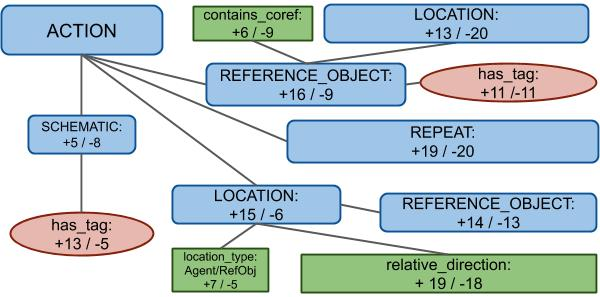
\includegraphics[width=\linewidth ]{figures/ModelMistakesNarrow.jpg}
    \caption{\label{fig:mistakes} We show nodes in the grammar which are most often wrongly predicted, with false positive (+) and false negative counts (-).}
\end{figure}

\paragraph{Error Analysis: } We further investigate the errors of the Seq2seq models on one of the data splits. We find that the model still struggles with span predictions: out of 363 errors, 125 only make mistakes on spans (and 199 get the tree structure right but make mistakes on leaves). Figure~\ref{fig:mistakes} shows the nodes which are most commonly mistaken, with the number of false positive and false negatives out of these 363 mistakes. Unsurprisingly, the most commonly confused span leaf is ``has\_tag'', which we use as a miscellaneous marker. Aside from that ``has\_tag'' however, the span mistakes are evenly spread over all other leaves. The next most common source of mistakes comes from the model struggling between identifying whether a provided location corresponds to the target of the action or to the reference object, and to identify instructions which imply a repetition. The former indicates a lack of compositionality in the input representation: the model correctly identifies that a location is mentioned, but fails to identify its context. Repeat conditions on the other hand challenge the model due to the wide variety of possible stop condition, a problem we suggest future work pay special attention to.



\section{Conclusion}
In this work, we have described a grammar over a mid-level interface for a Minecraft assistant. We then discussed the creation of a dataset of natural language utterances with associated logical forms over this grammar that can be executed in-game. Finally, we showed the results of using this new dataset to train several neural models for parsing natural language instructions.  %We find that the models we trained were able to fit the templated data nearly perfectly, but were less accurate on human-generated data.  v
Consistent with recent works, we find that BERT pre-trained models do better than models trained from scratch, but there is much space for improvement.
We believe this data will be useful to researchers studying semantic parsing, especially interactive semantic parsing, human-robot interaction, and even imitation and reinforcement learning. The code, dataset and annotation tools described in the paper have been open-sourced \footnote{\url{https://github.com/facebookresearch/craftassist/tree/master/acl2020_submission}}. 



% The problem of using a small amount of parsed human data with the infinite generations of our grammar to improve results on human-distribution; or otherwise building models that can generalize to the human distributions is an exciting area for future work.   
%More generally, we hope that the grammar, templates, and human data will be useful to researchers studying human-robot and human assistant interaction.  


%and hope that future work tackling the task presented here may produce better results.

\clearpage

\bibliography{refs}
\bibliographystyle{acl_natbib}

\clearpage

\appendix

\label{sec:supplemental}
\section{Basic Data Cleanup}
\label{sec:data_cleanup}
We threw away all duplicate commands in the dataset and only got annotations for unique commands from each data source.

We performed post-processing on the text by first inserting spaces between any special character (brackets, ``,'', ``x'') followed by alphanumeric character. For example ``make a 5x5 hole'' was post-processed to ``make a 5 x 5 hole'' and ``go to (1,2,3)'' to ``go to ( 1 , 2 , 3 )''. We then used the tokenizer from spaCy \url{https://spacy.io/}  to tokenize every word in the sentence.

When constructing logical forms: we threw away any keys with values : `None' , `Other' or `Not Specified' . Our tool allows workers to select these options when annotating. We skipped stopwords and articles like `a' , `an' etc when constructing spans of children. We reordered the indices of words in spans to always be from left to right (regardless of which order the words were selected in the sentence when annotating).

For commands annotated as ``composite'' (meaning a command that requires multiple actions), we set up another tool where we asked crowd-sourced workers to split the composite command into individual commands. Each of these commands were then sent to our web-based tool described in \ref{sec:annotation} and the results were combined together under the key: ``action\_sequence'' by preserving the order. So in the sentence: ``jump twice and then come to me'', we first have the sentence split into commands: ``jump twice'' and ``come to me'' and then combine  their logical forms together under ``action\_sequence'' so we first have the ``Dance'' action followed by ``Move'' action. This tool is described in Section \ref{sec:composite}.
\clearpage
\onecolumn

\section{Crowd-sourced task and tools instructions}
\label{sec:instructions}
This section covers details of each crowd sourced task we've described in the paper along with screenshots of the web-based annotation tool described in \ref{sec:collected_data}.

\subsection{Image and Text Prompts}
\label{sec:freegen_instructions}
In this task we showed a screenshot of the bot and environment to the crowd-sourced workers and asked them to give us free-form commands for the assistant.
The instructions shown to workers are shown in \ref{fig:freegen}.
\begin{figure}
	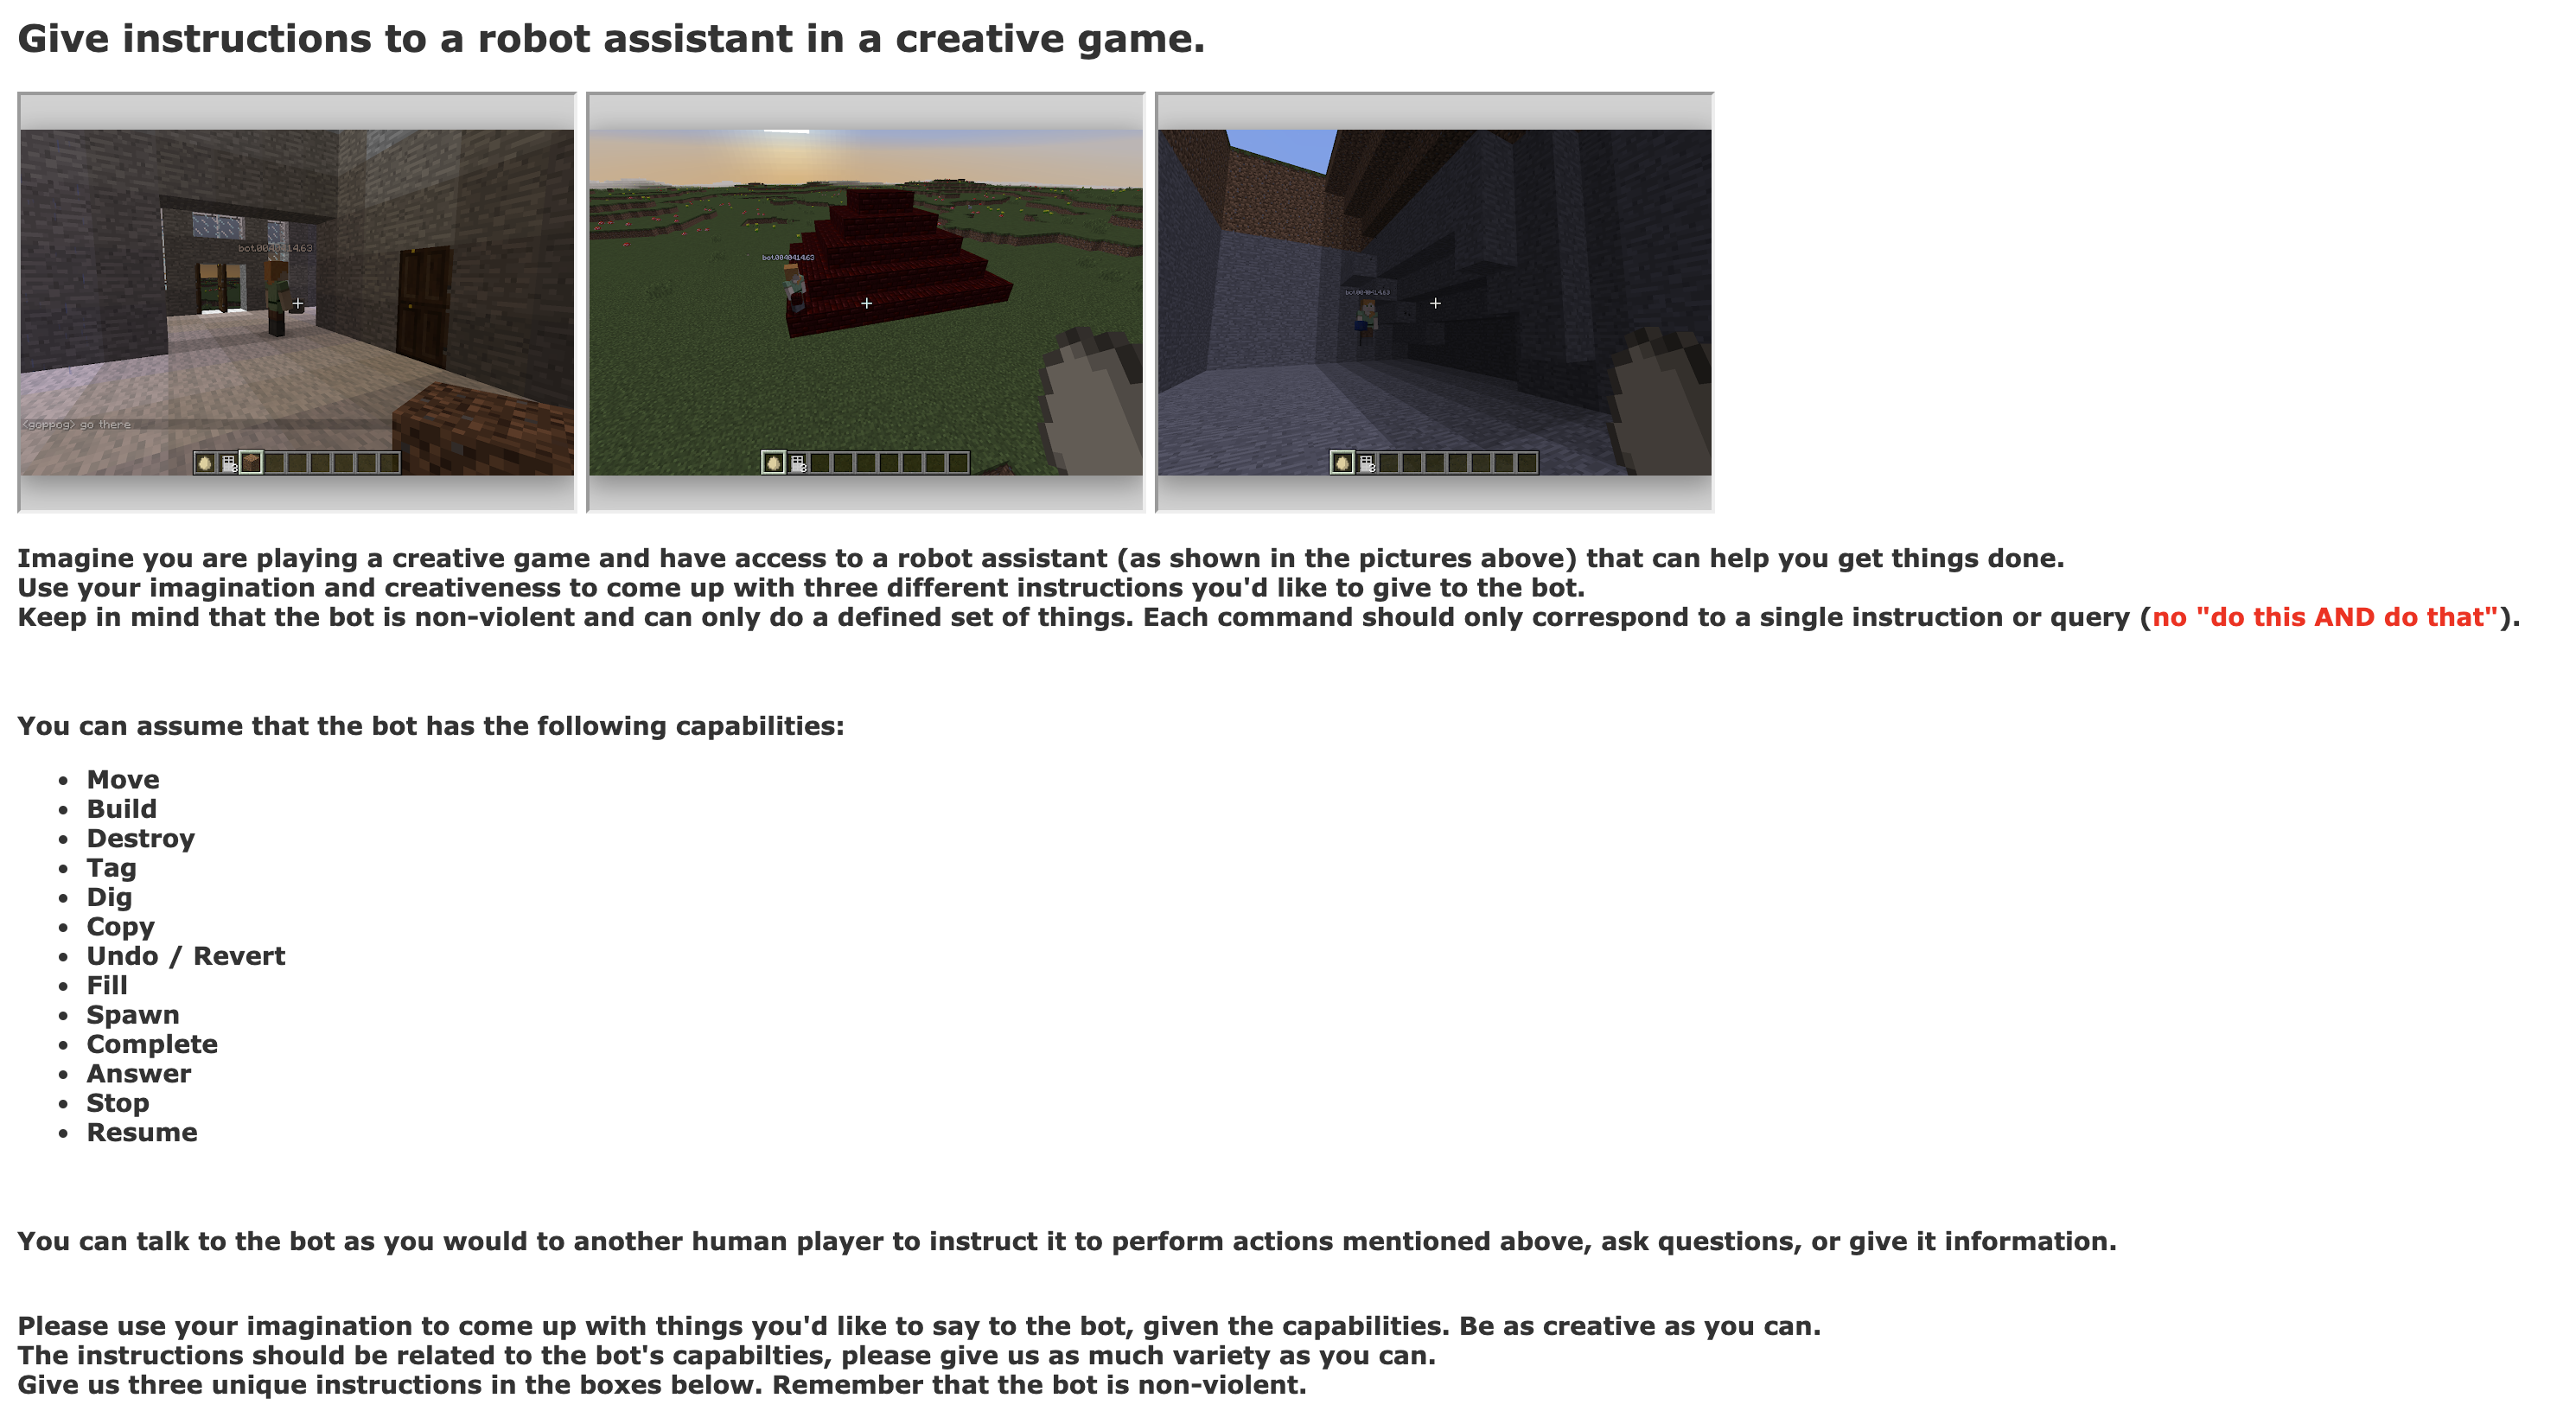
\includegraphics[width=\linewidth ]{figures/freegen.jpg}
	\caption{The task instructions shown to crowd-sourced workers for the Image and text prompts task\label{fig:freegen}}
\end{figure}

\subsection{Interactive Gameplay}
\label{sec:appen}
In this task we had crowd-sourced workers play with our bot and interact with it using in-game chat. 
The instructions shown to workers are shown in \ref{fig:appen}. 
\begin{figure}
	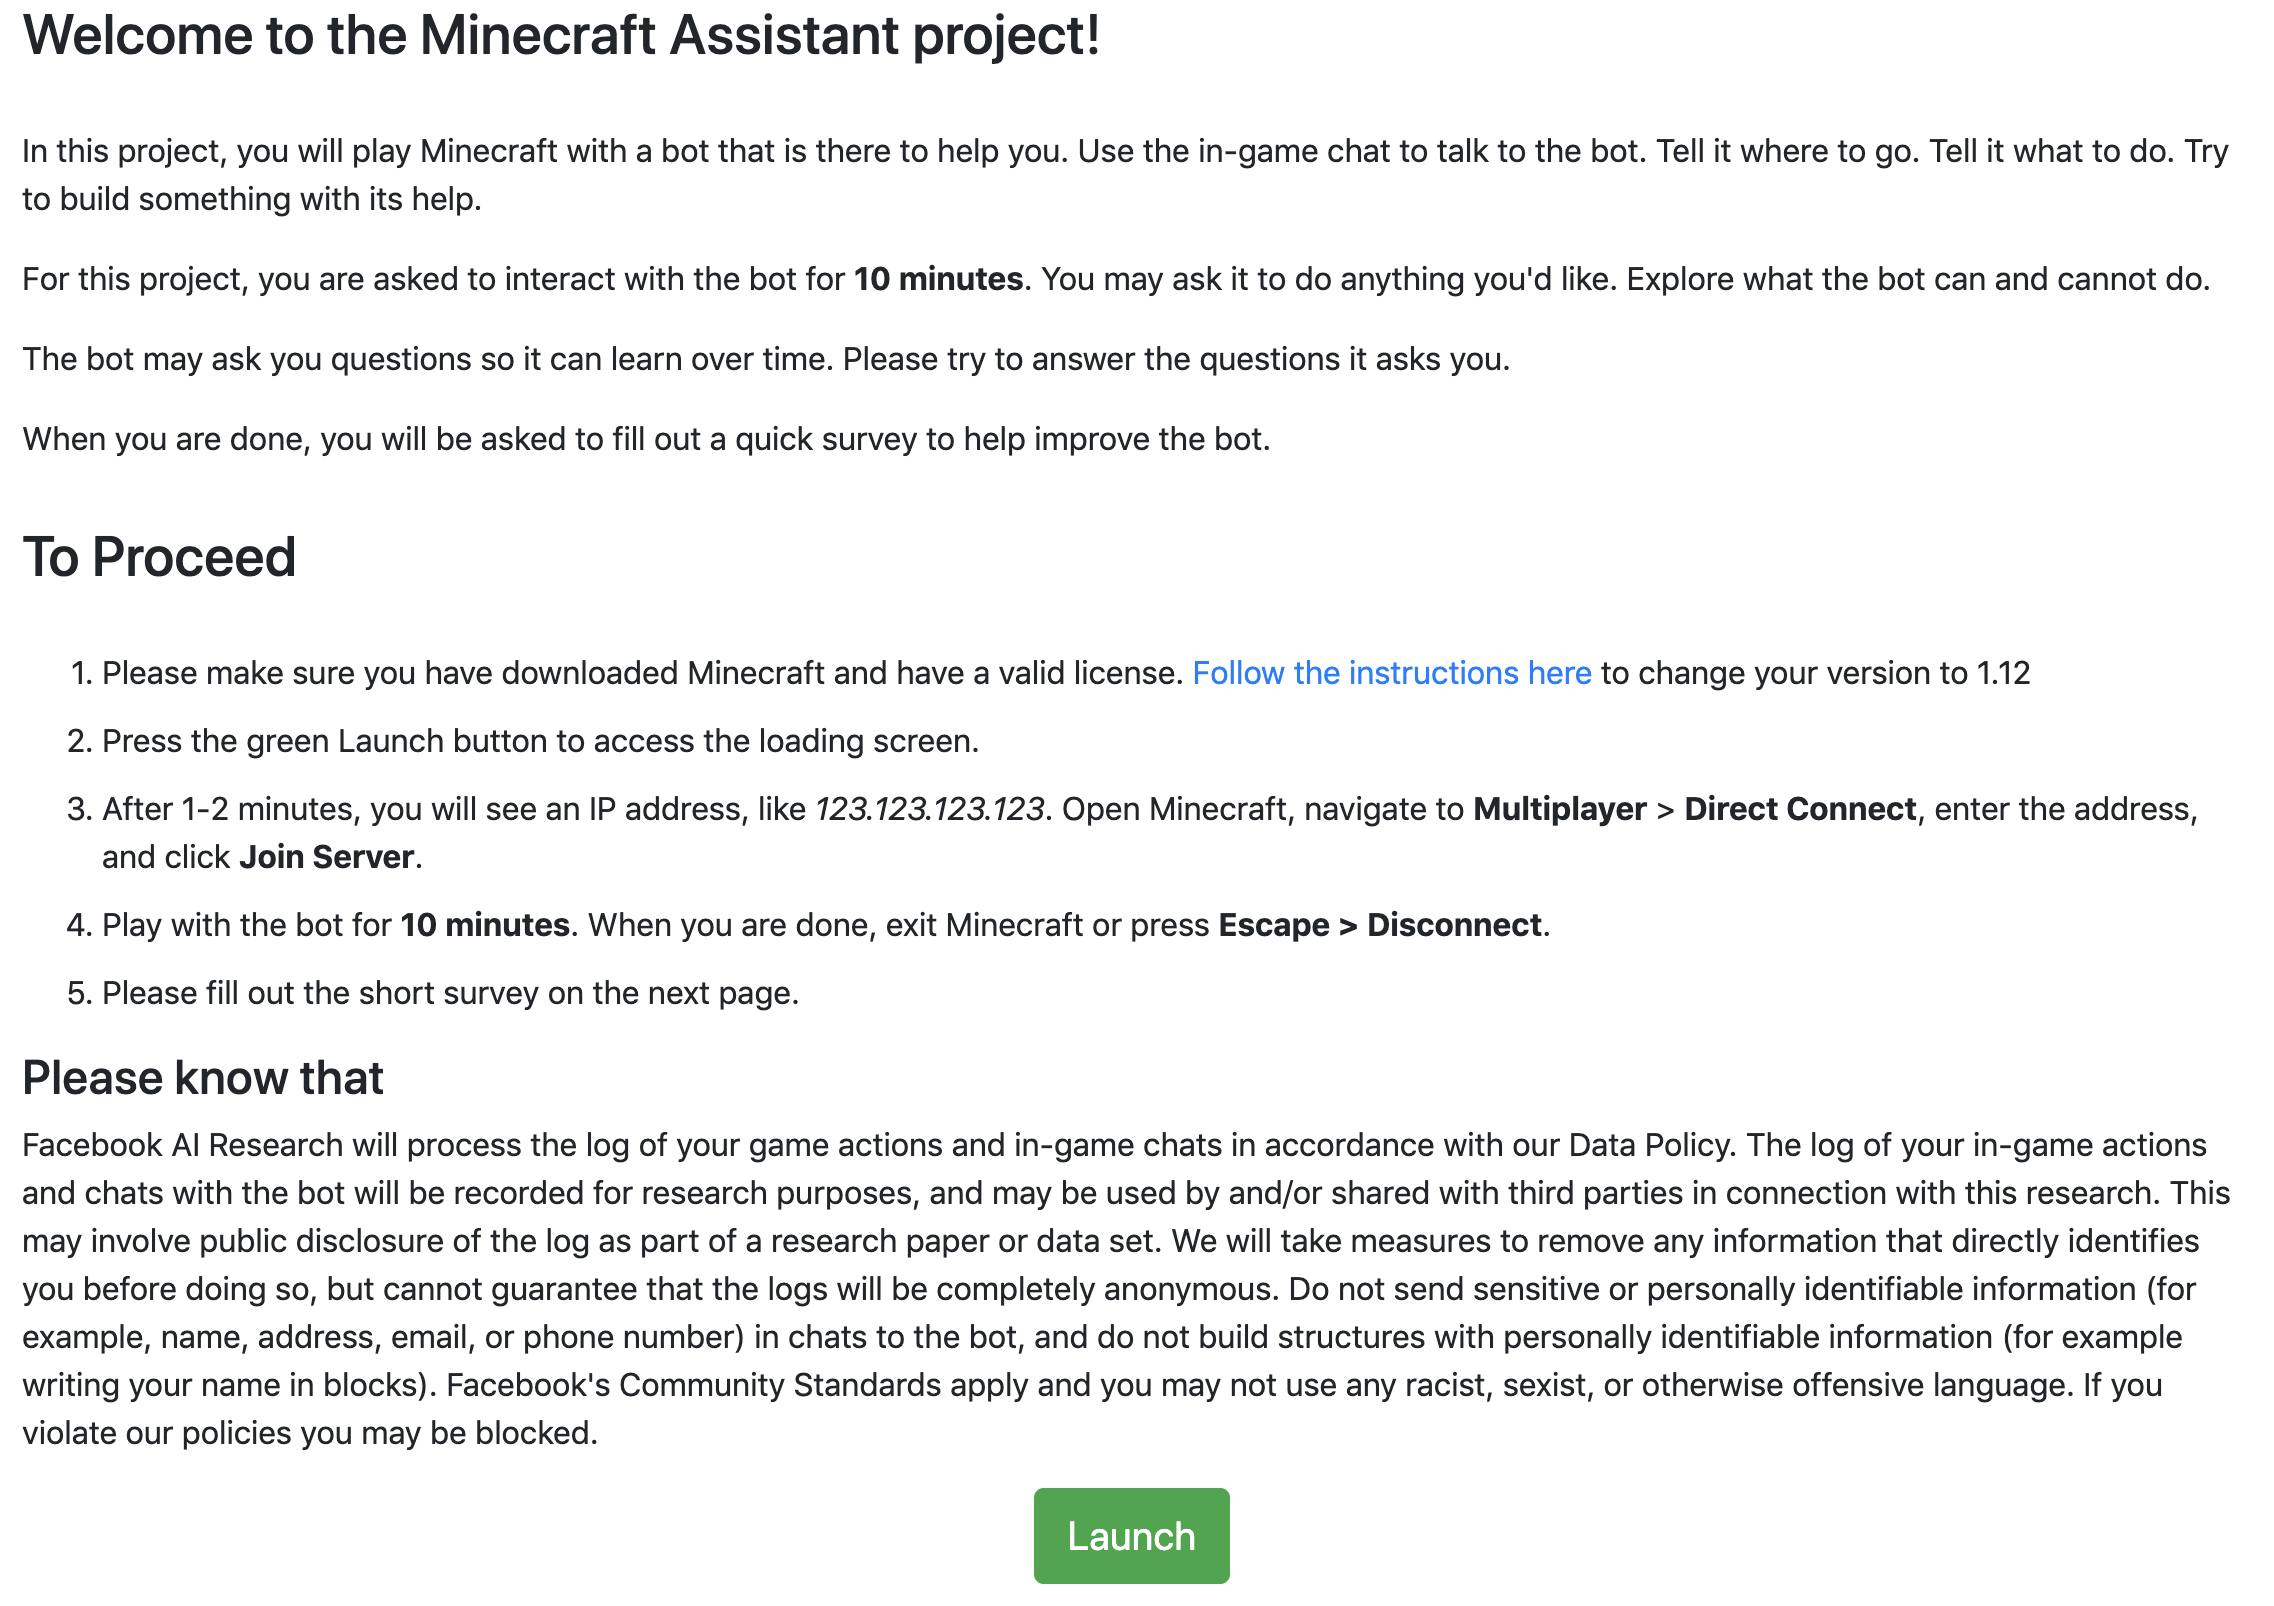
\includegraphics[width=\linewidth ]{figures/appen.png}
	\caption{The task instructions shown to crowd-sourced workers for the interactive game play\label{fig:appen}}
\end{figure}

\subsection{Annotation tool}
\label{sec:anntn}
The web based annotation tool has two subparts: Tool a and Tool b.
\subsubsection{Tool a}
This tool is the first tool in the process of annotation and asks crowd-sourced workers to help determine the intent (dialogue\_type or action\_type) of the sentence and highlight other pieces of the text based on the choices they made for the intent. (For example: if the intent was ``Build'' they are asked to select words for the thing to be built  and the location respectively.)
We also provided helpful tooltips with examples at every step of the process.

The instructions shown to workers for Tool a are shown in figure \ref{fig:annotation_task1} and step by step annotation process is shown in figure \ref{fig:annotation_step1}
\label{sec:tool_a}
\begin{figure}
	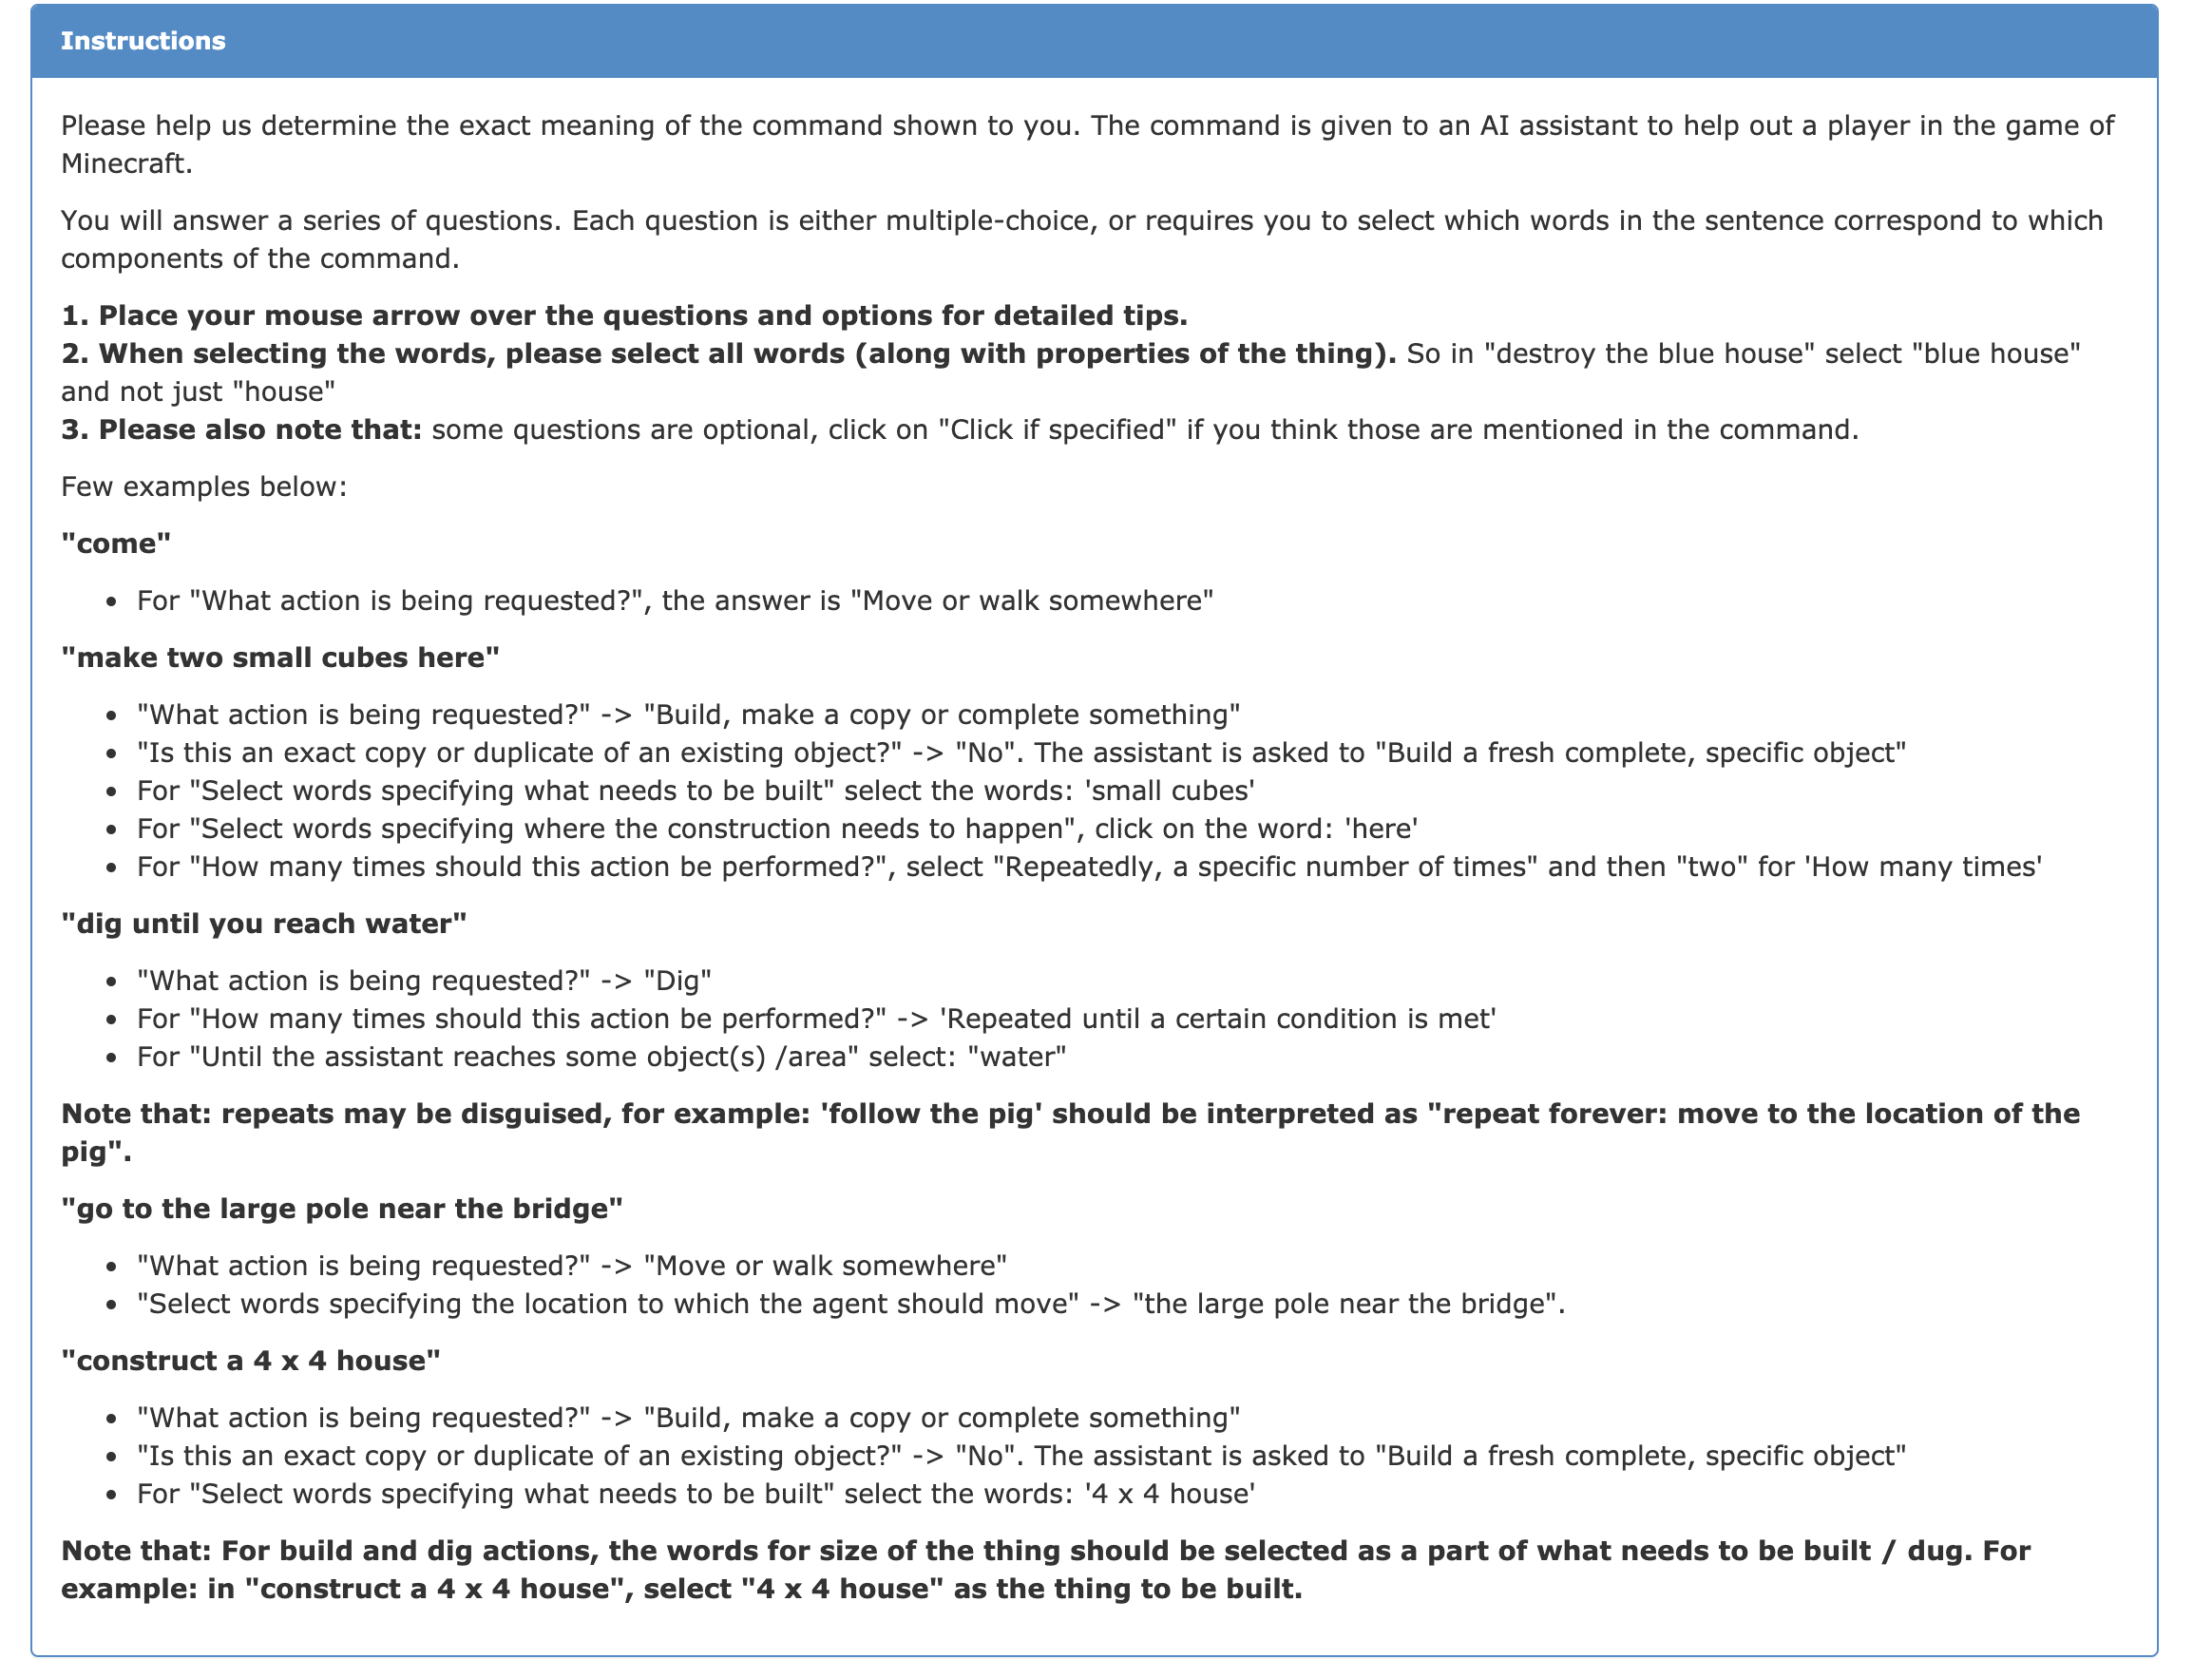
\includegraphics[width=\linewidth ]{figures/11.png}
	\caption{The task instructions shown to crowd-sourced workers for the annotation Tool a}
	\label{fig:annotation_task1}
\end{figure}

\begin{figure}[h]

    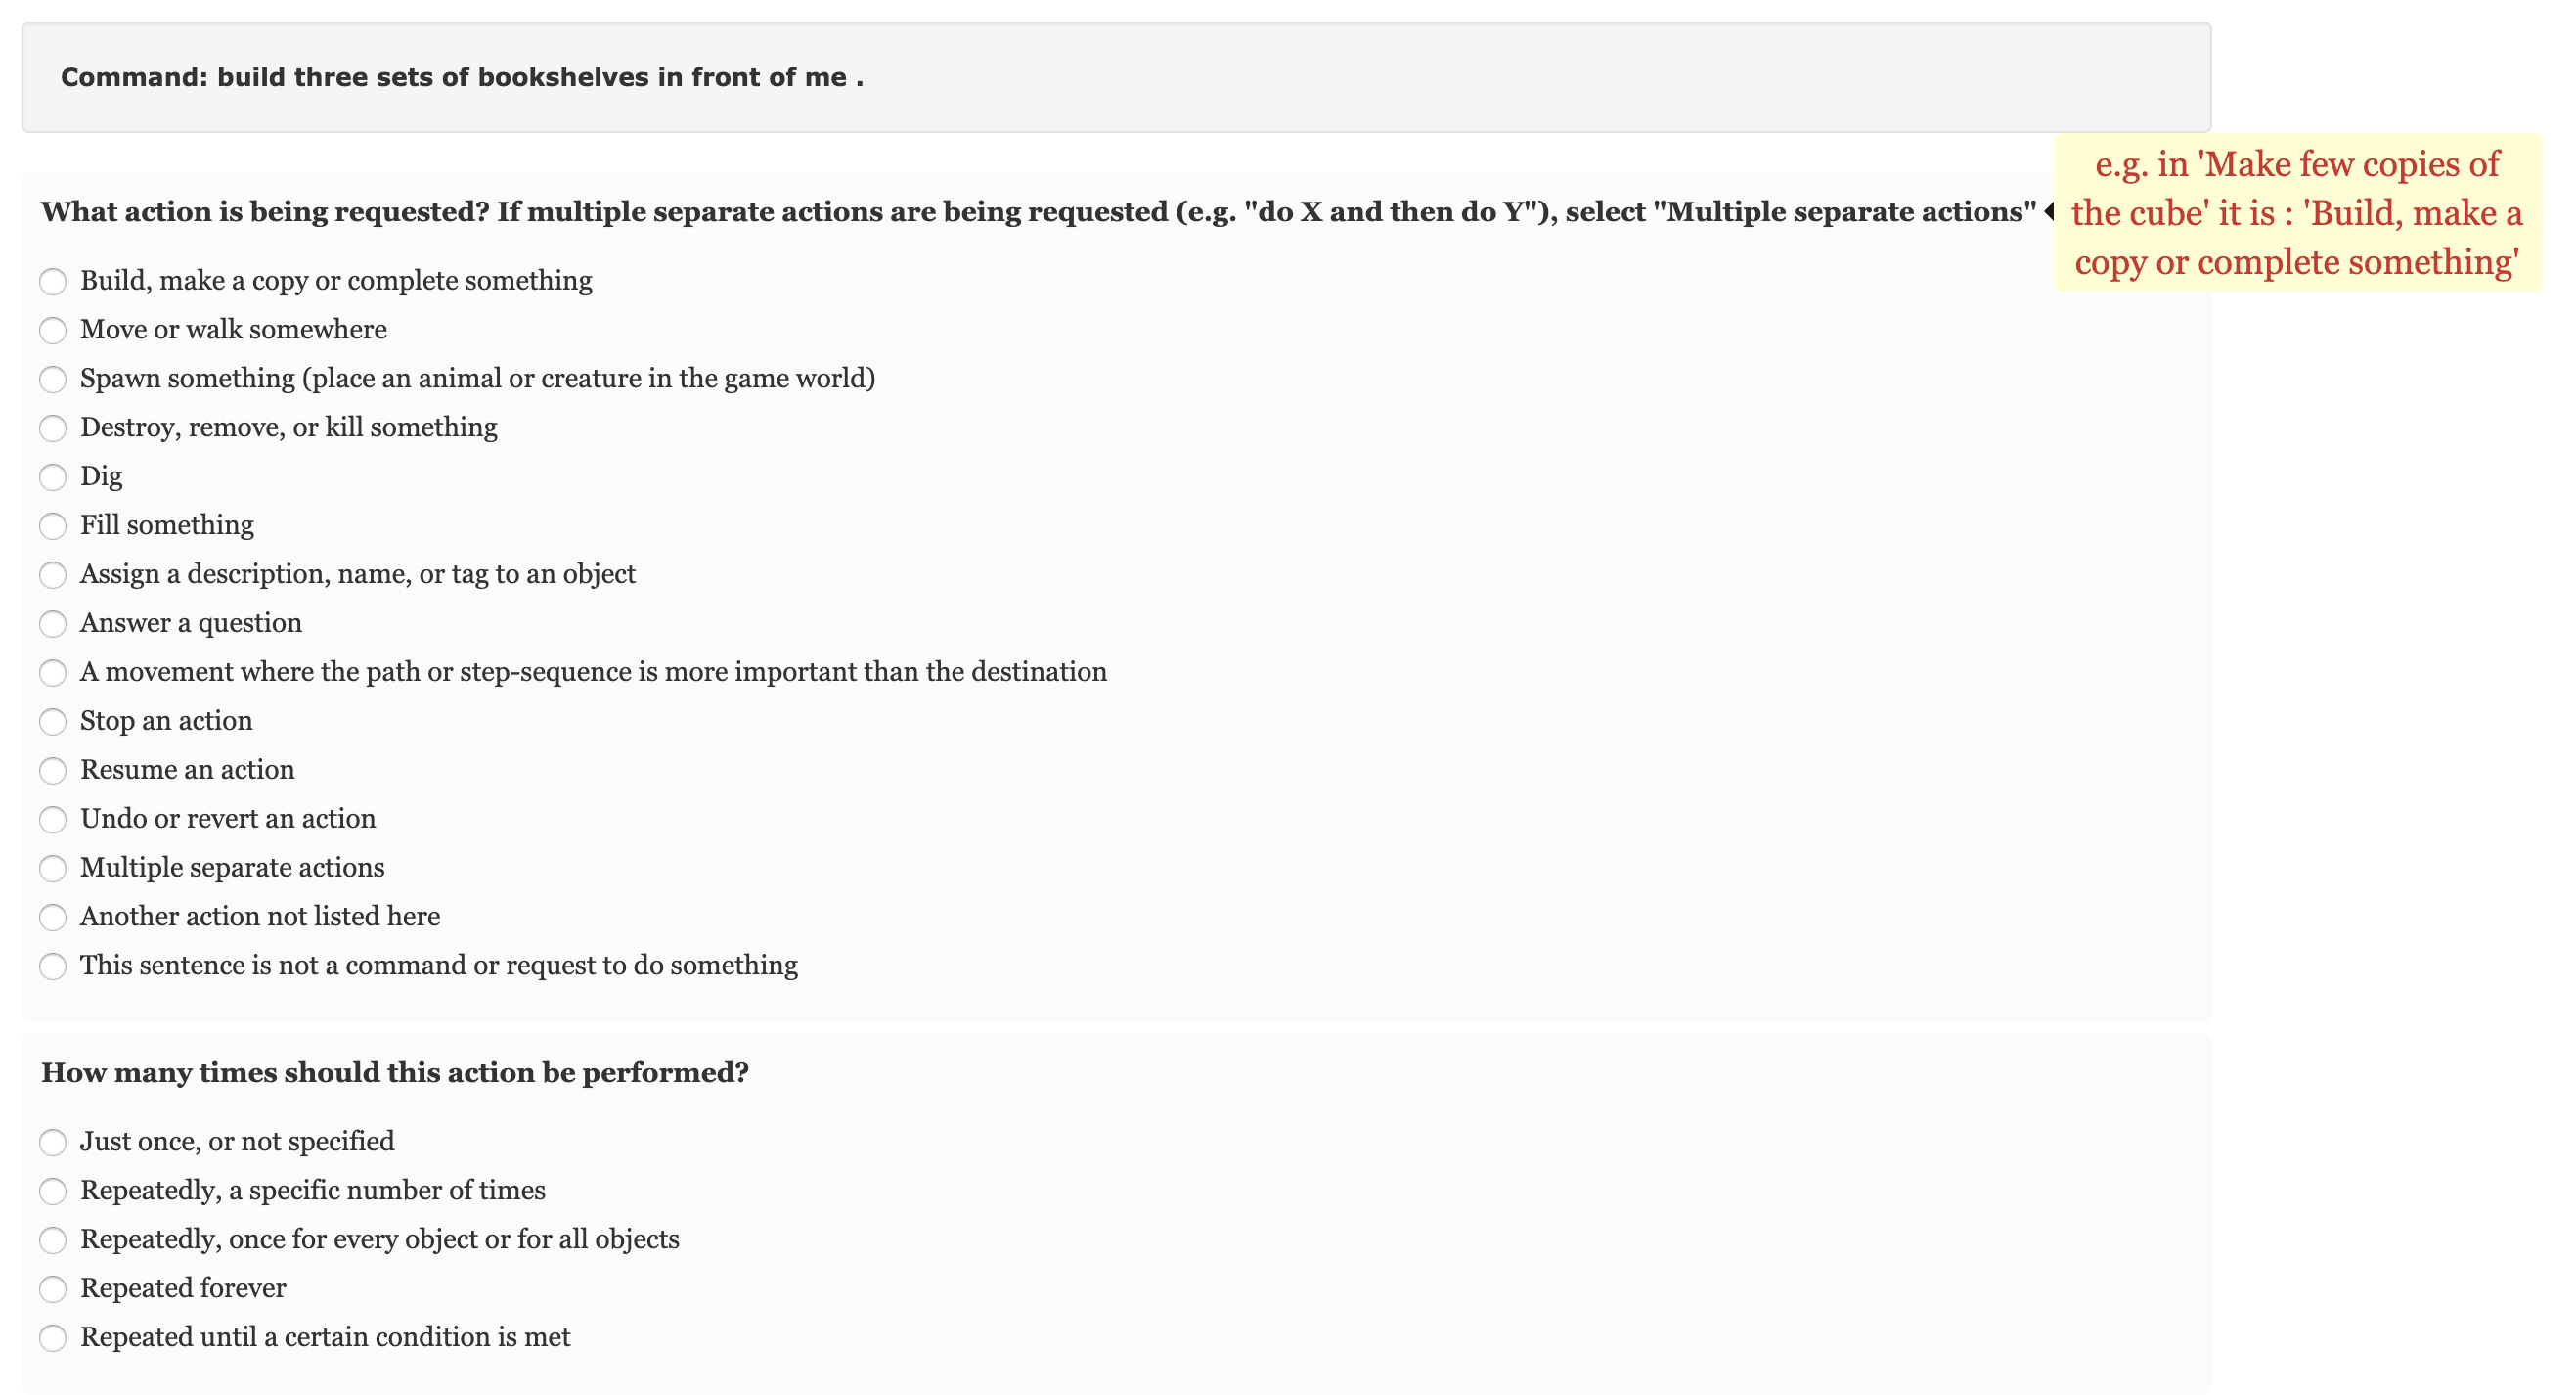
\includegraphics[width=\linewidth, height=6cm, ,keepaspectratio  ]{figures/12.png}
    \bigbreak
     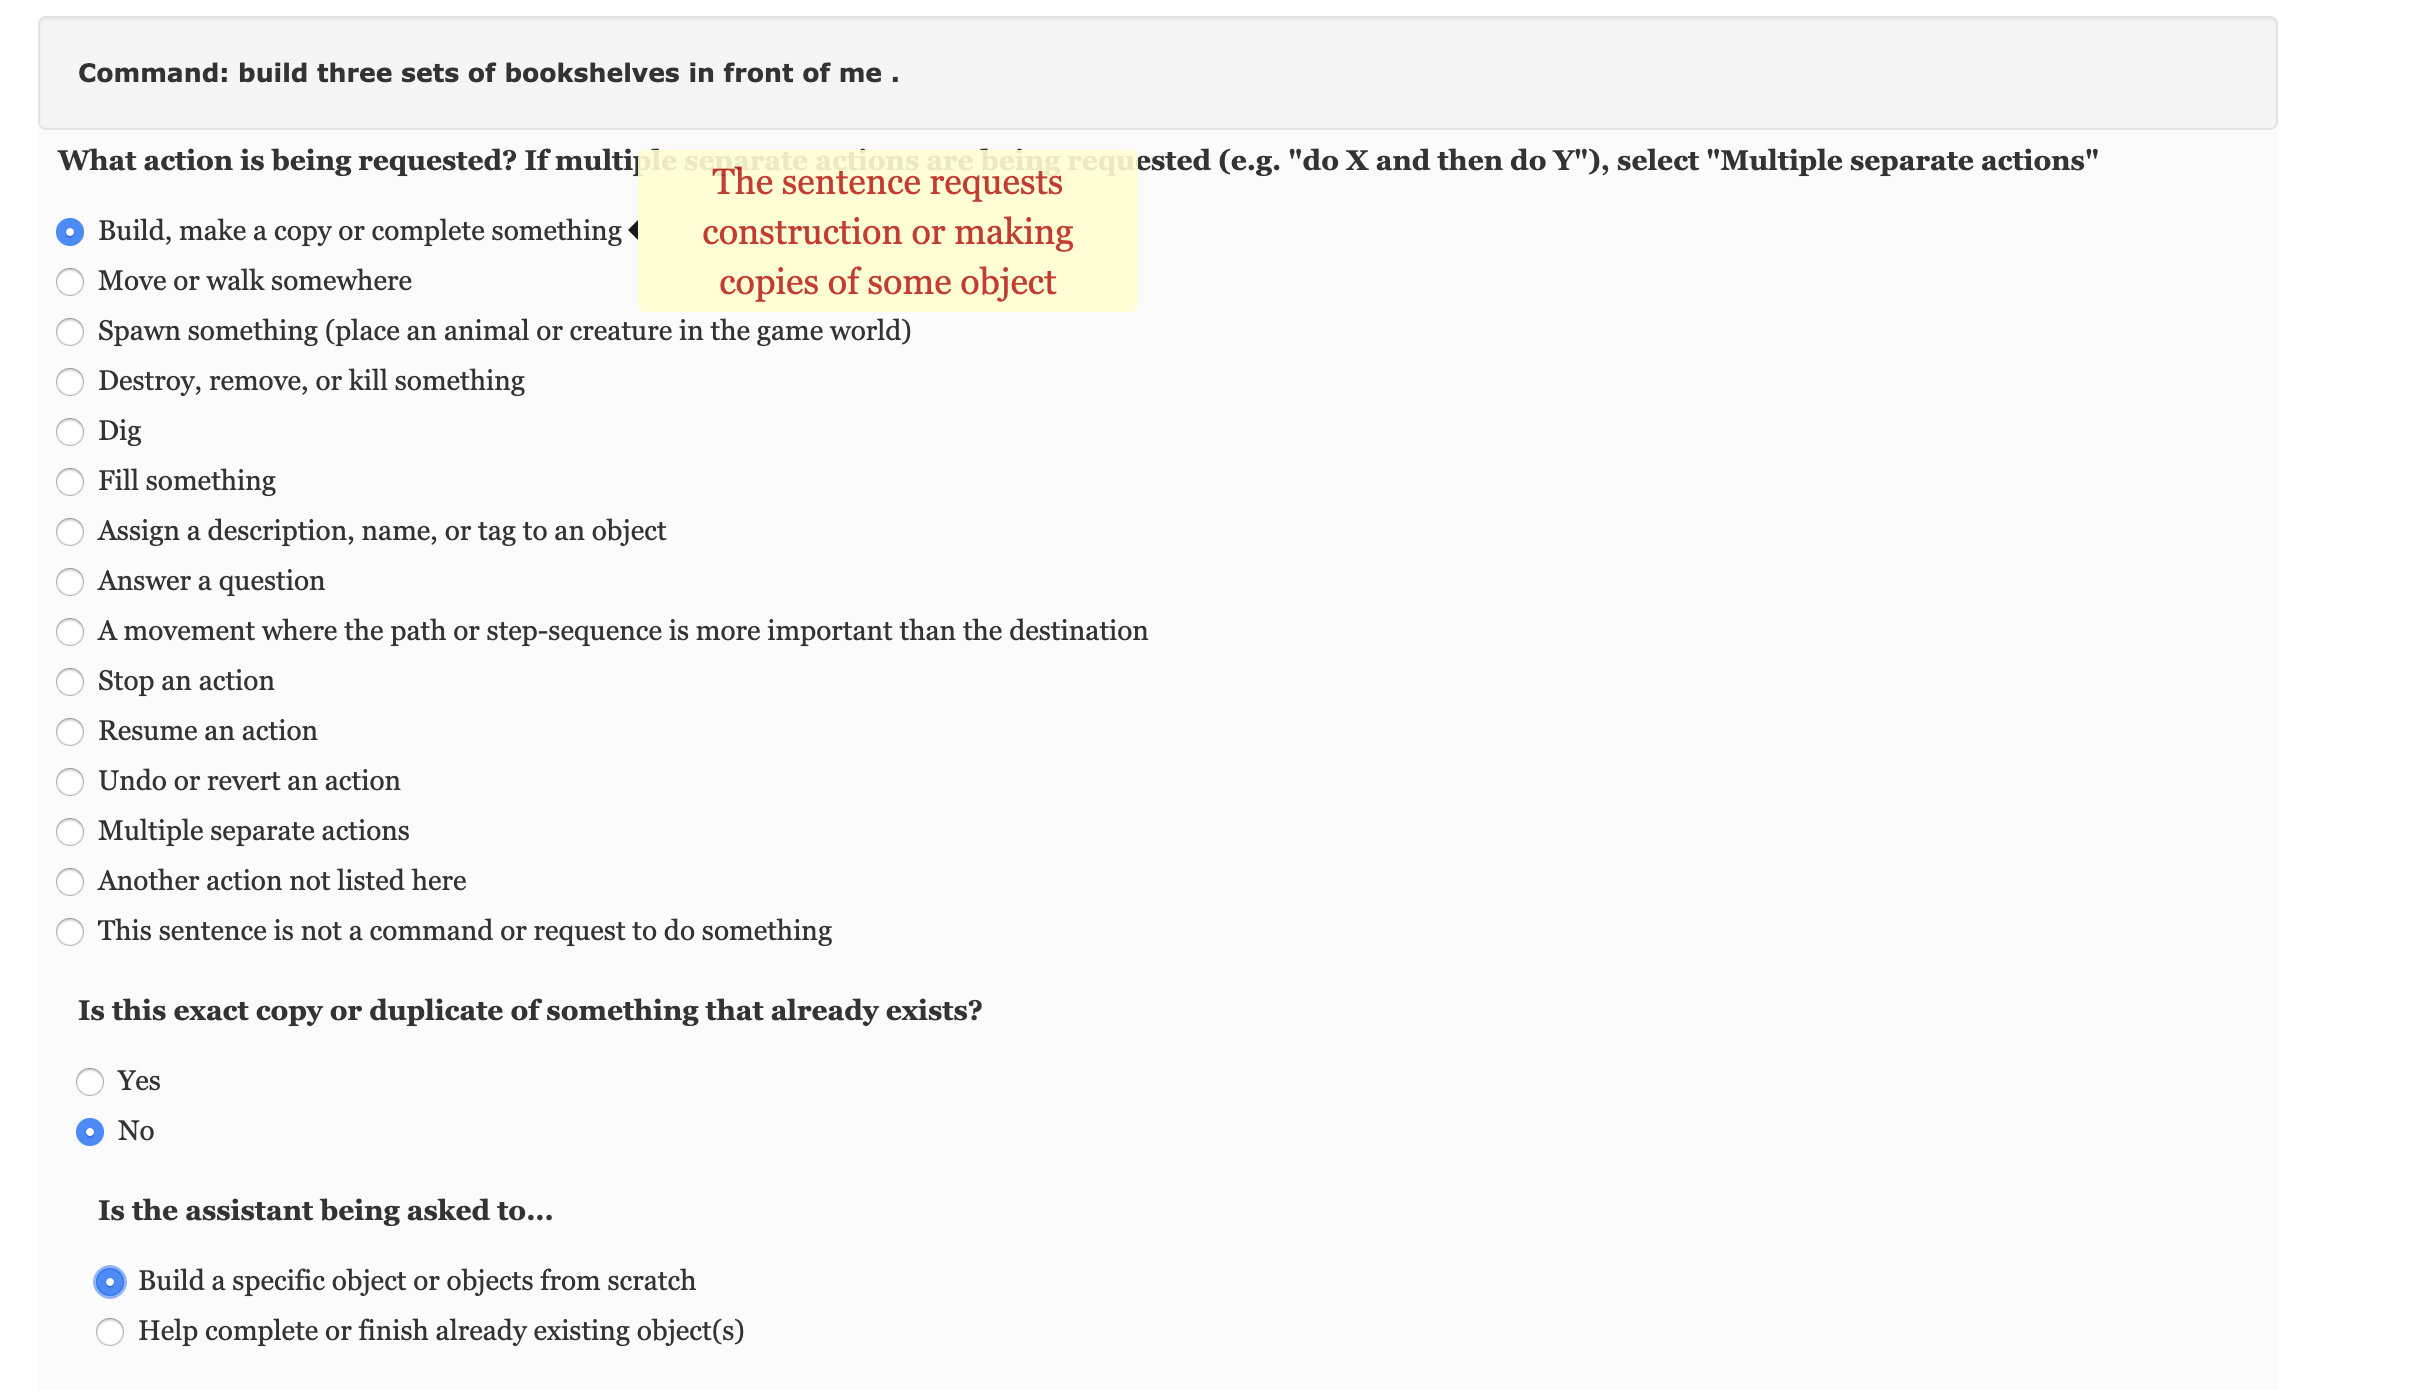
\includegraphics[width=\linewidth, height=6cm, ,keepaspectratio  ]{figures/13.png} 
     \bigbreak
     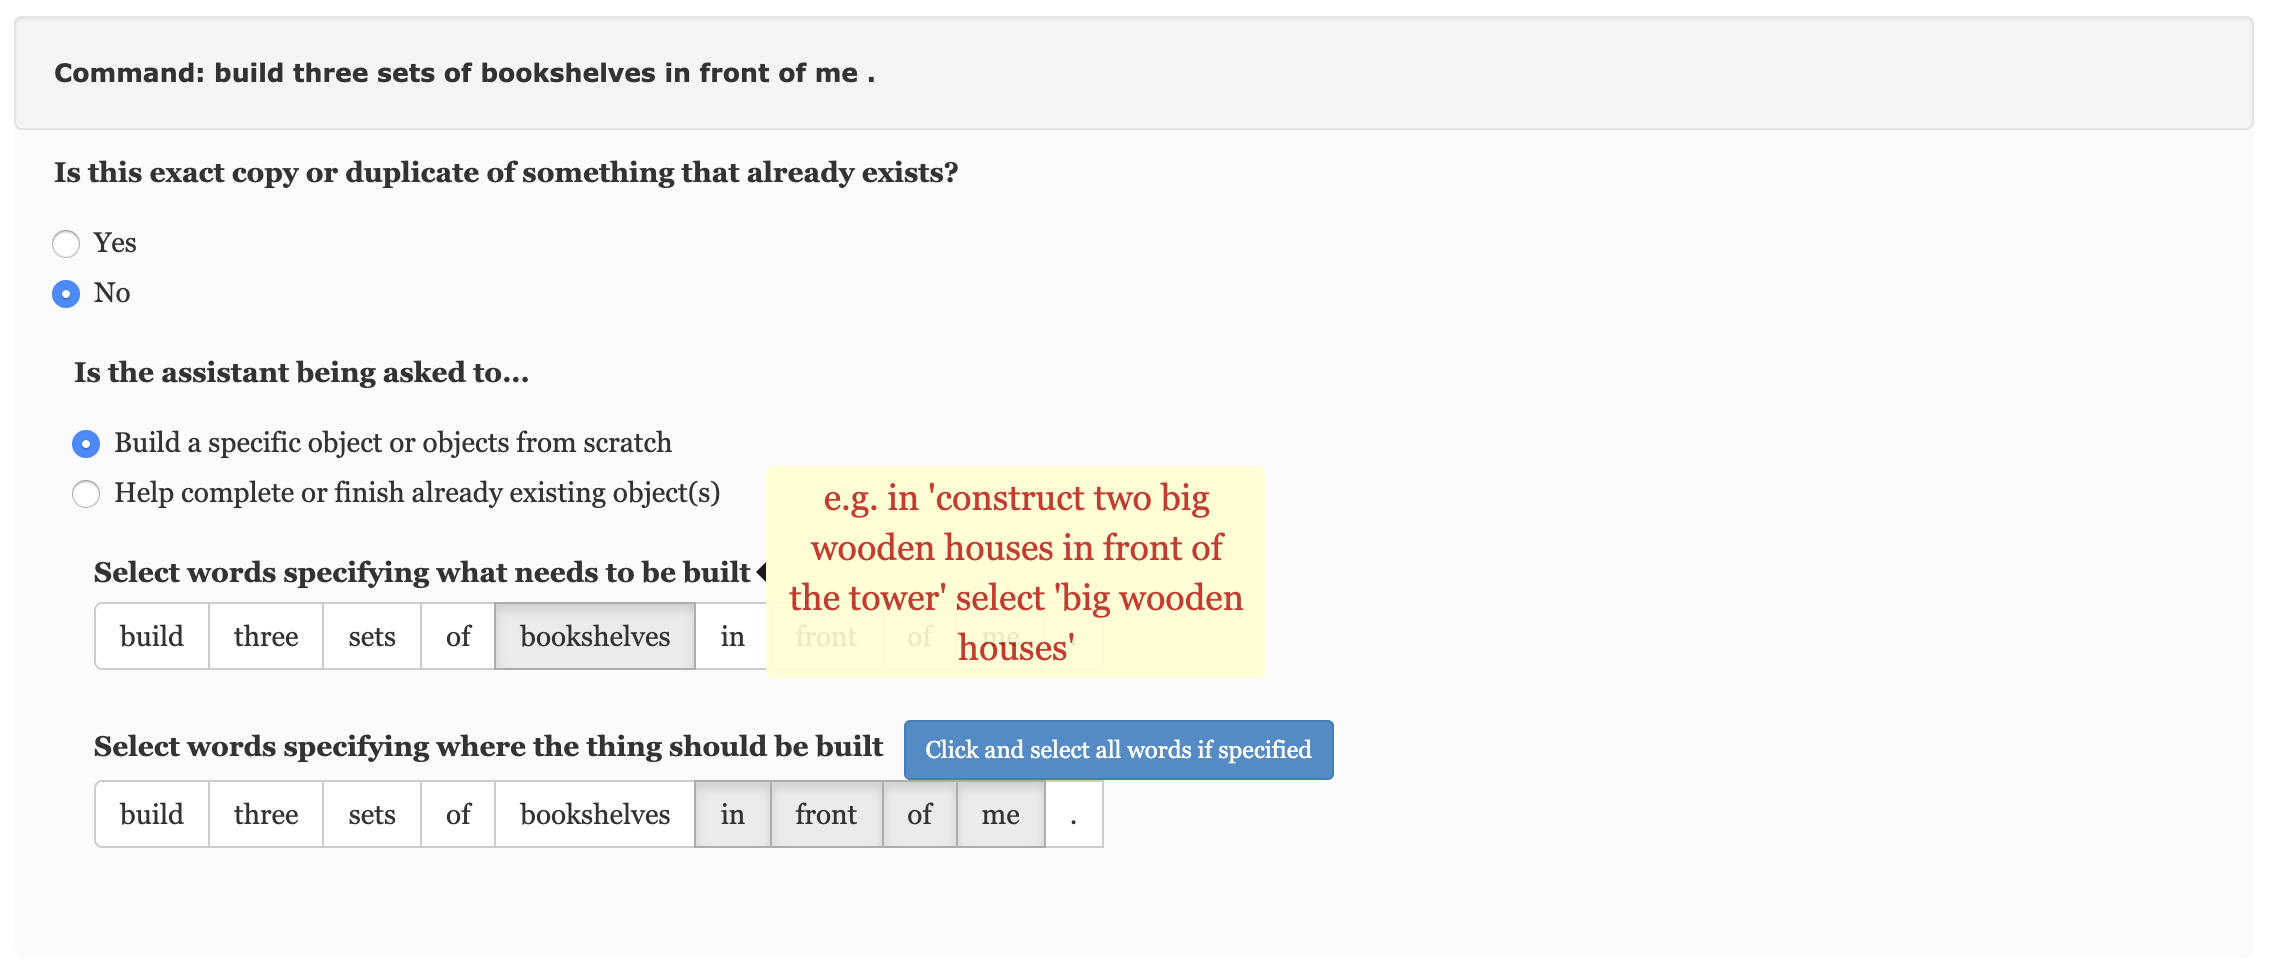
\includegraphics[width=0.65\linewidth, height=6cm, ,keepaspectratio ]{figures/14.png}
     \bigbreak
     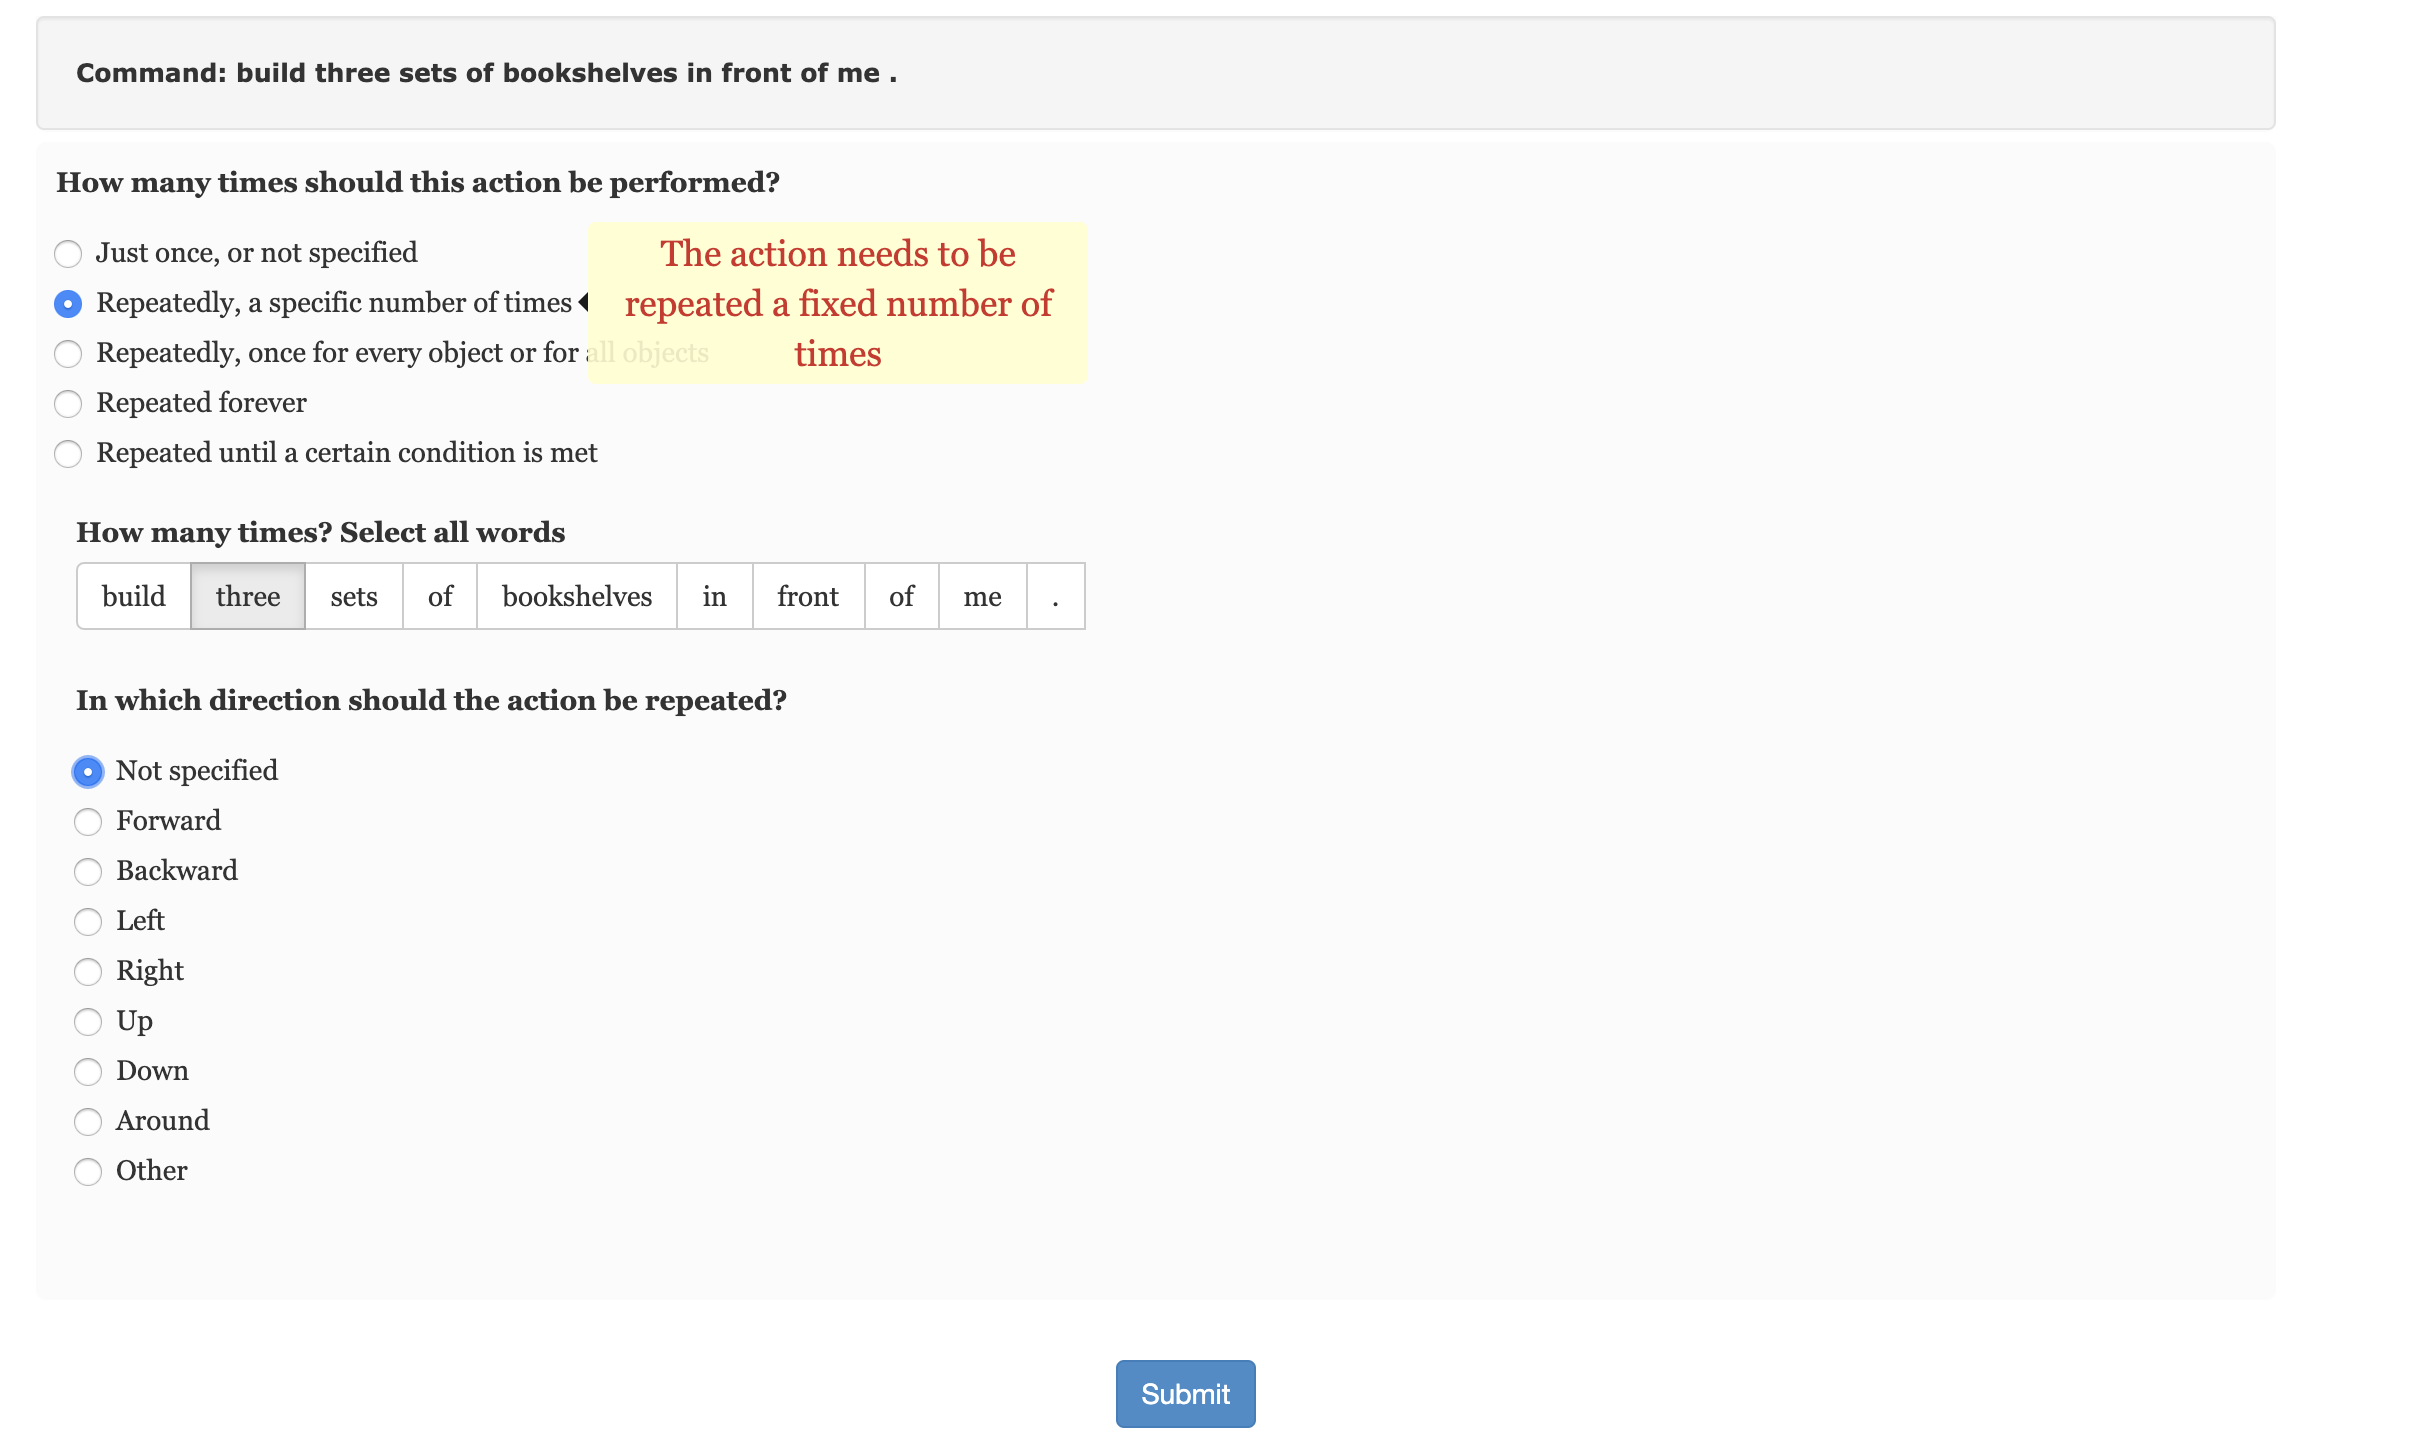
\includegraphics[width=\linewidth, height=6cm, ,keepaspectratio]{figures/15.png}
	 \caption{The step by step screenshot of annotations process for the command: ``build three sets of bookshelves in front of me .''  in Tool a}
	\label{fig:annotation_step1}
\end{figure}

\subsubsection{Tool b}
After we determine the intent from Tool a and get highlighted span of words for respective children of the intent, we use this tool.
This is the second tool in the annotation process and asks crowd-sourced workers to help determine the fin-grained properties of specific entities of the action or dialogue. Note that we already got the words representing these, highlighted in \ref{sec:tool_a}. For example : the words `` big bright house'' are highlighted in the sentence ``destroy the big bright house by the tree '' as an outcome of Tool a.
The questionnaire changes dynamically based on the choices the workers make at every step of the tool. We provided helpful tooltips with examples at every step of the annotation process.
Using the output of Tool a and Tool b, we can successfully construct the entire logical form for a given sentence.

The instructions shown to workers for Tool b are shown in Figure \ref{fig:annotation_task2} and step by step annotation process for annotating properties of ``location'' in a ``Move'' action is shown in Figure \ref{fig:move_location} and annotating ``reference\_object'' in ``Destroy'' action is shown in Figure \ref{fig:destroy_ref}
 

\label{sec:tool_b}

\begin{figure}
	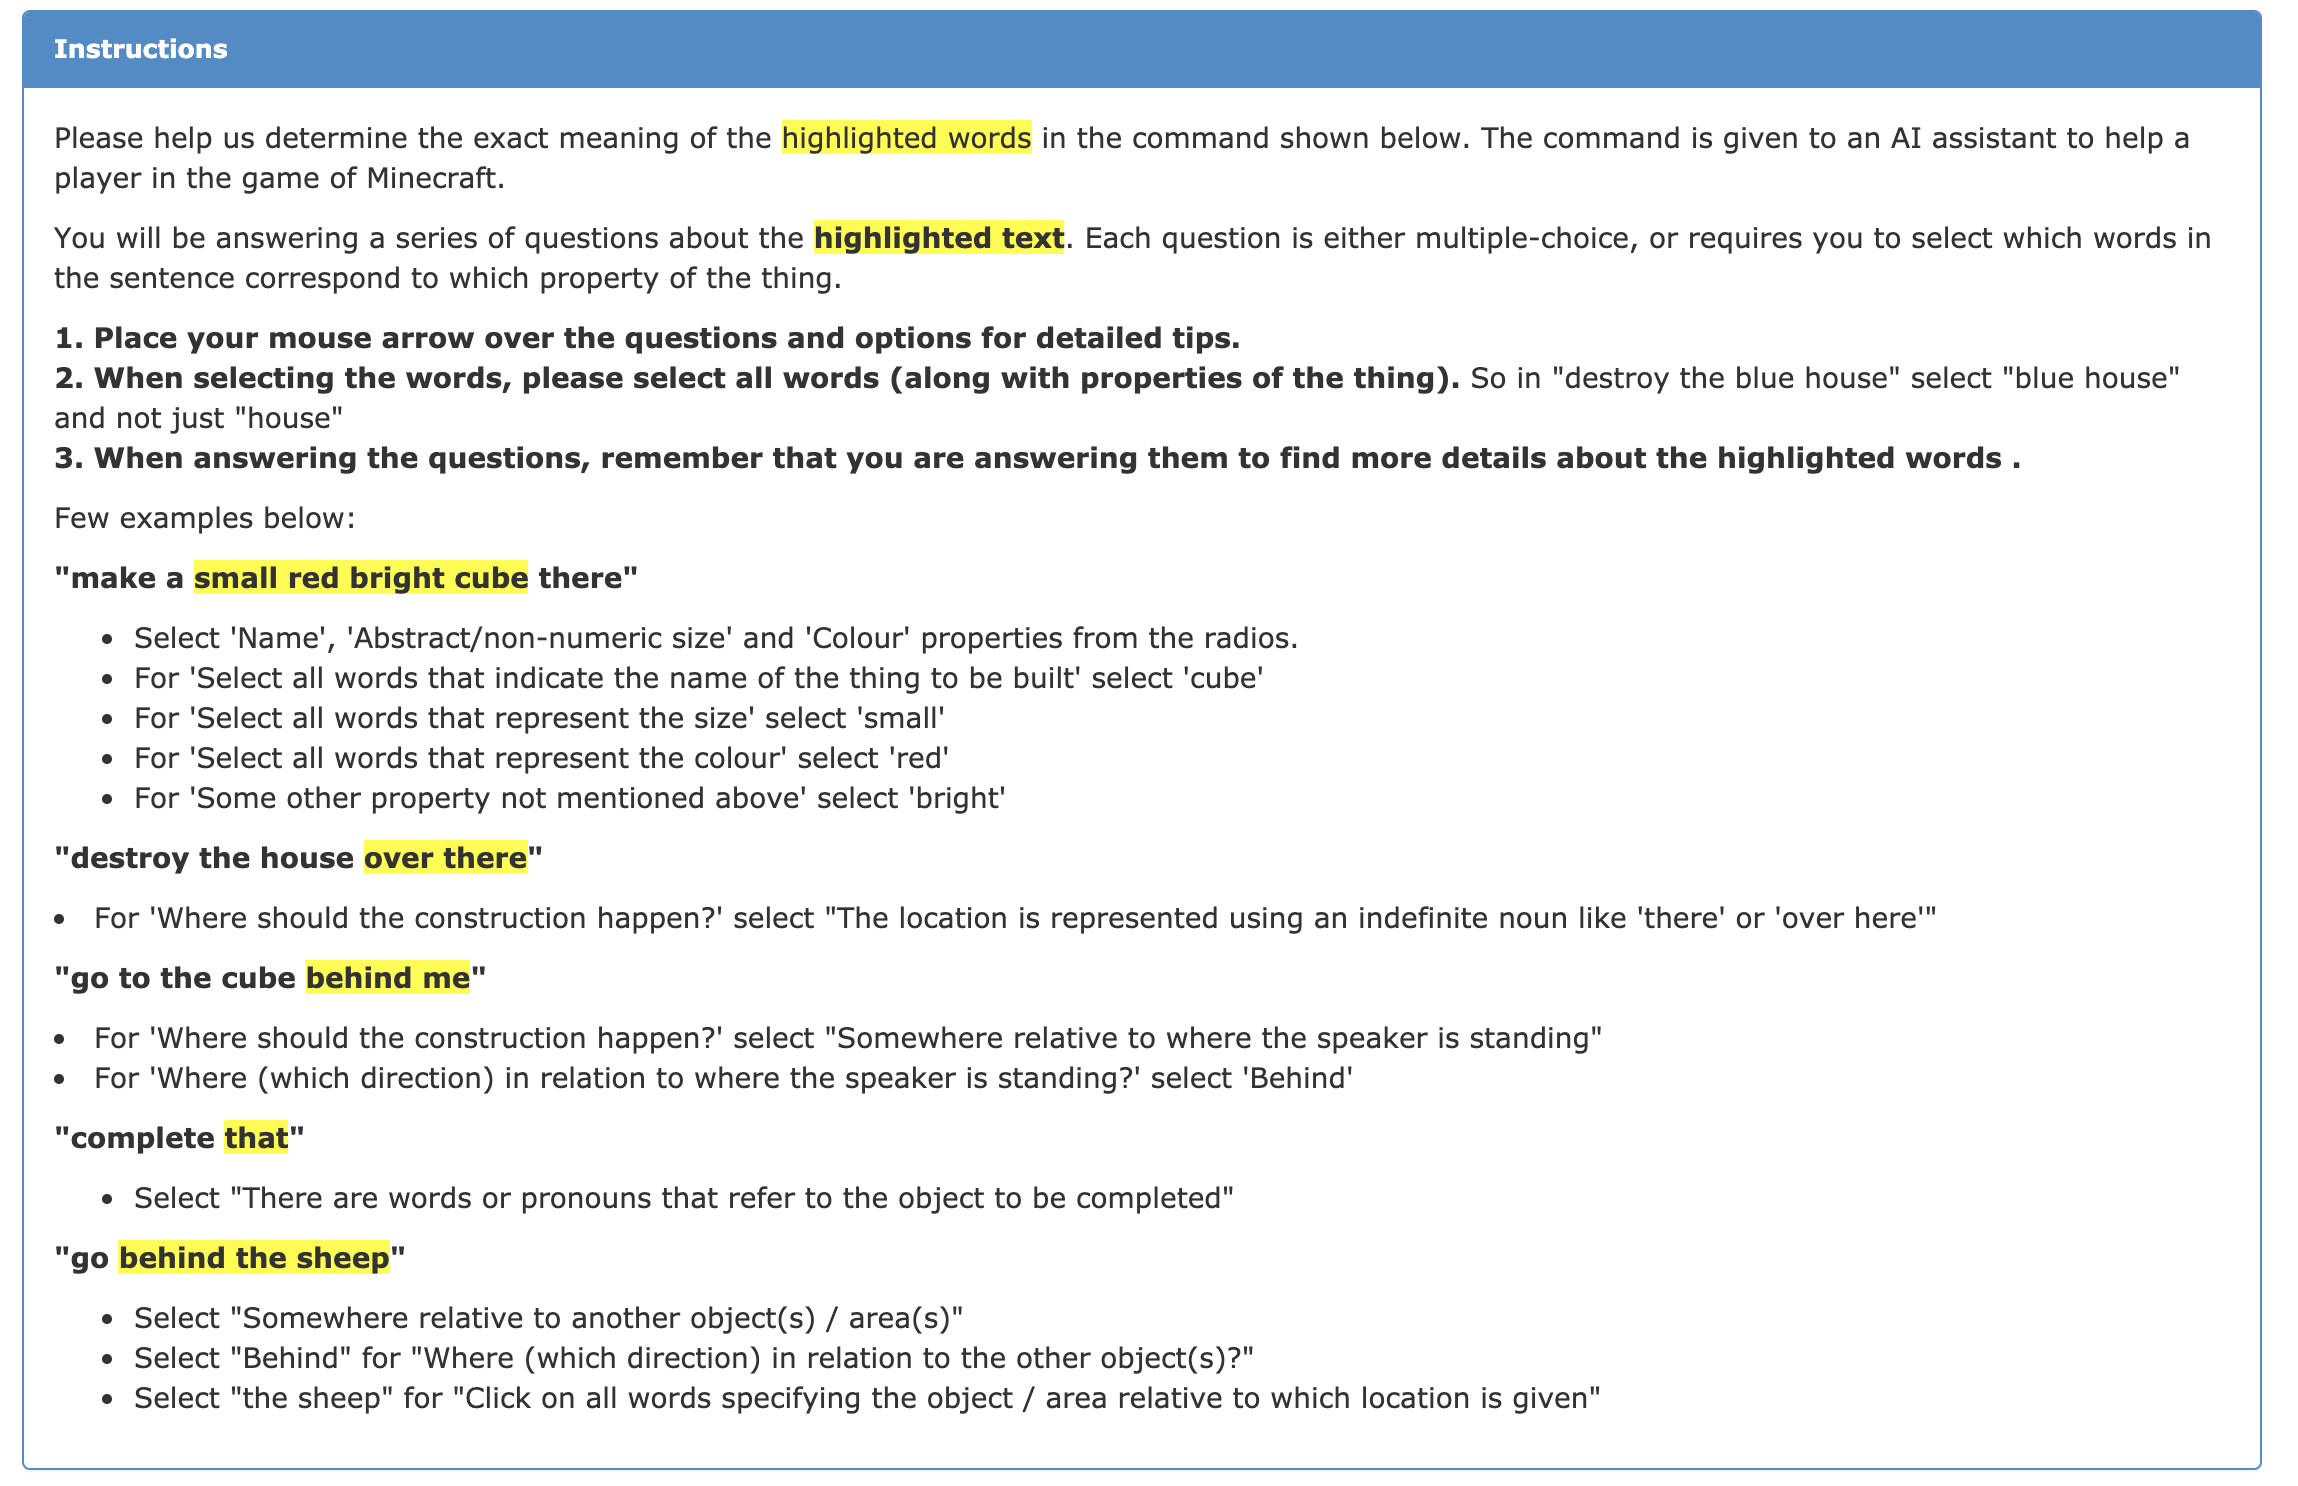
\includegraphics[width=\linewidth ]{figures/21.png}
	\caption{The task instructions shown to crowd-sourced workers for the annotation Tool b}
	\label{fig:annotation_task2}
\end{figure}

\begin{figure}[h]
    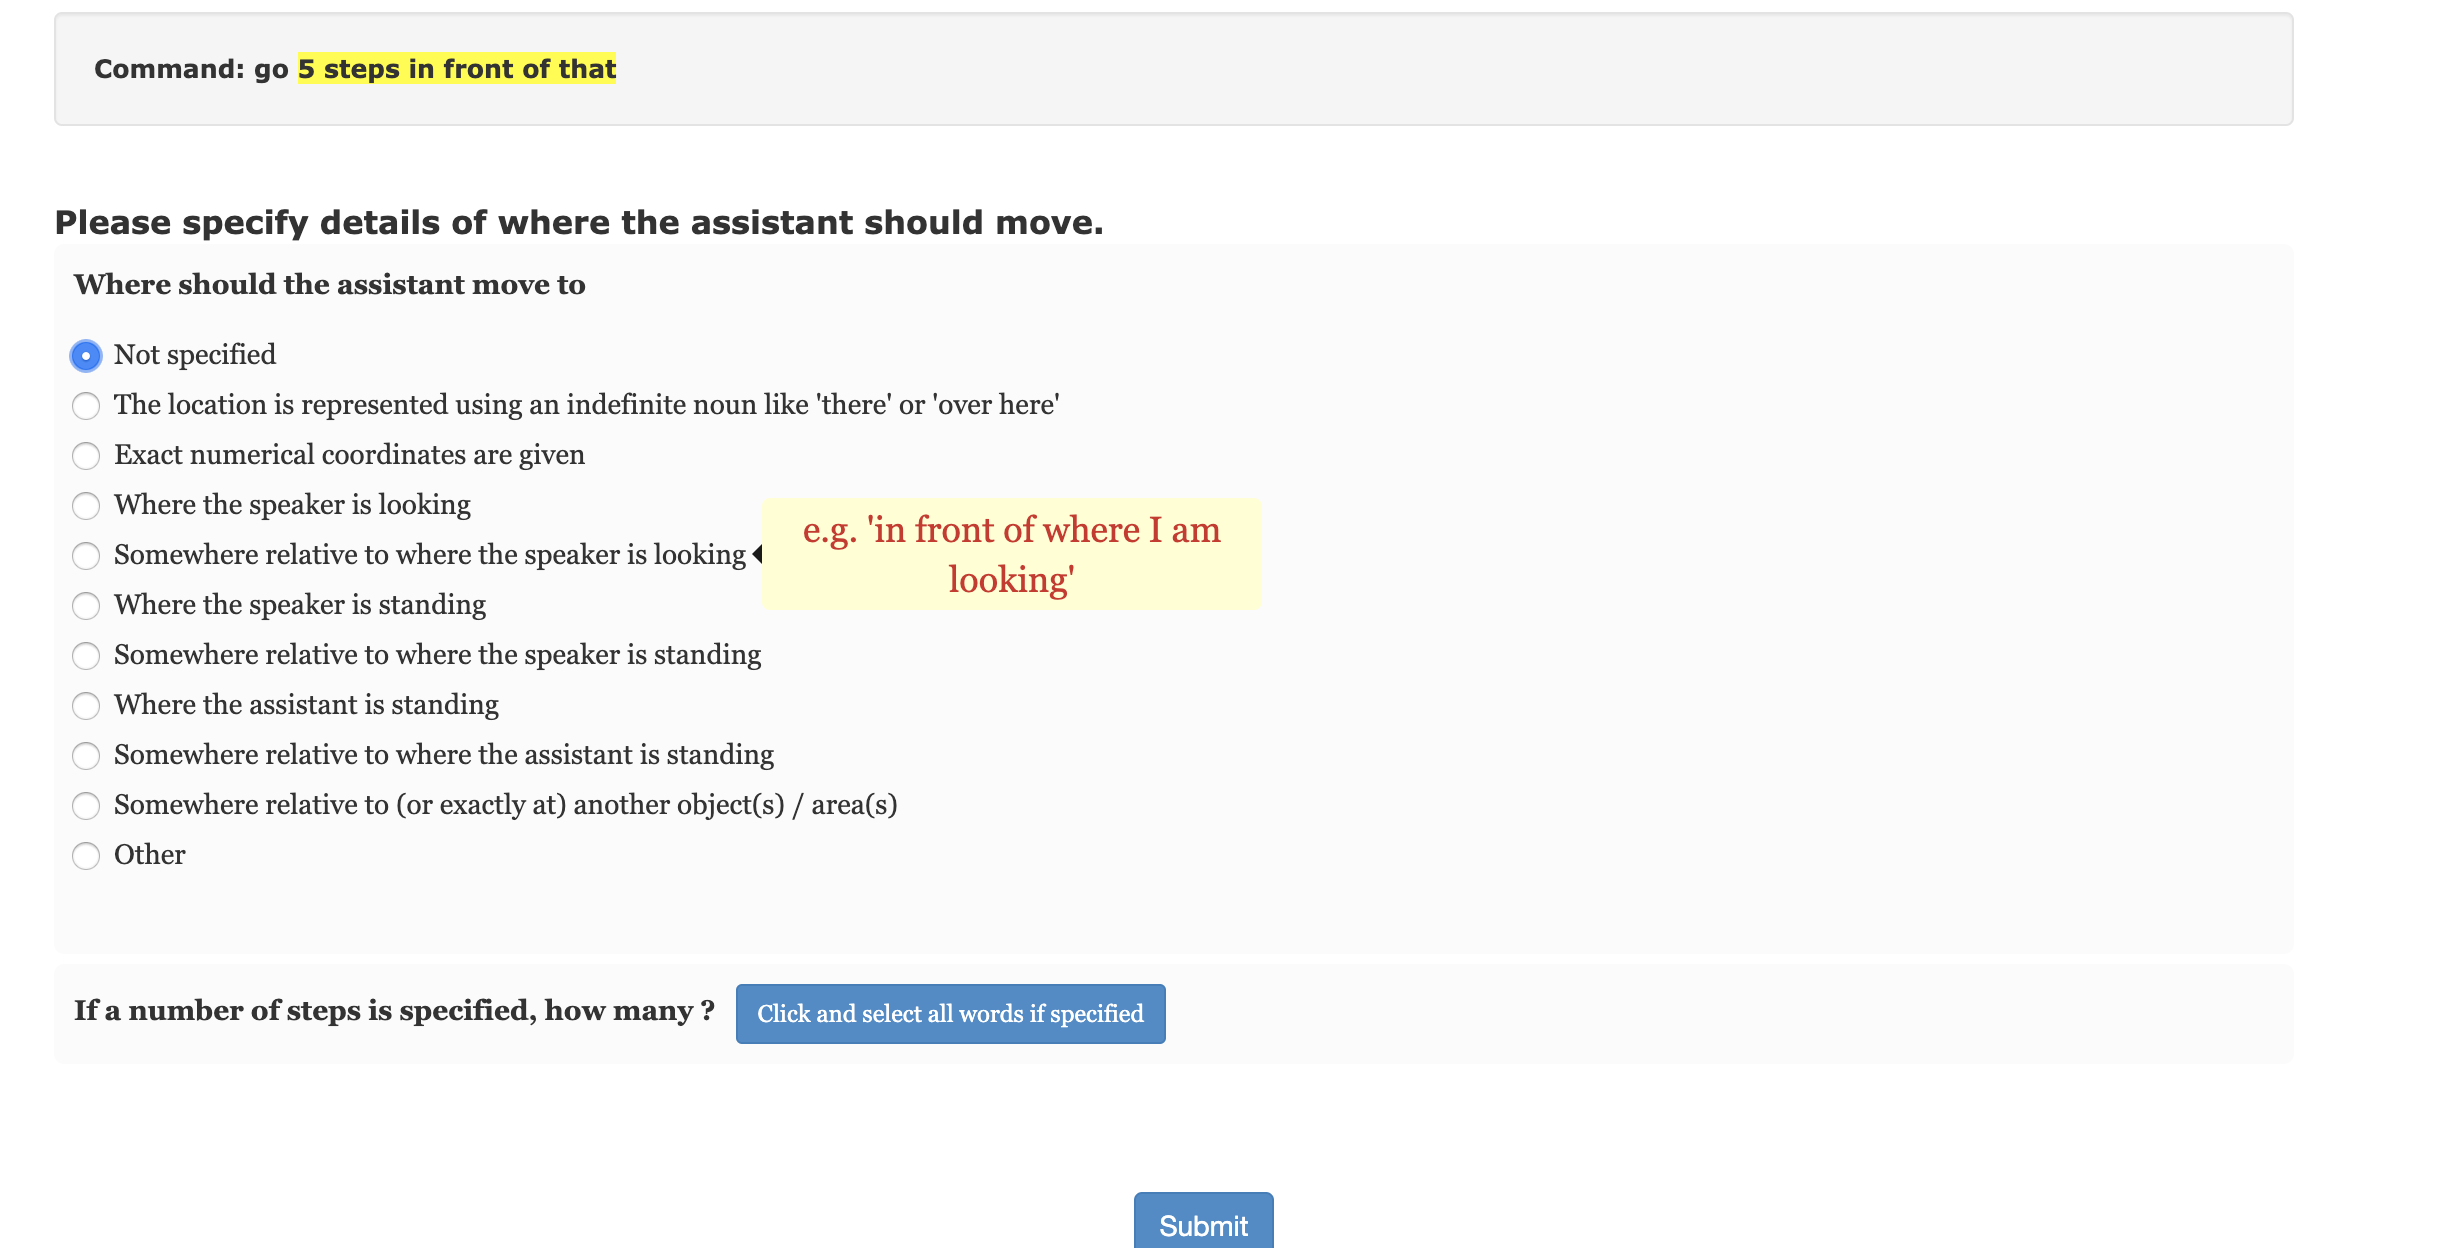
\includegraphics[width=\linewidth, height=6cm, ,keepaspectratio  ]{figures/22.png}
    \bigbreak
     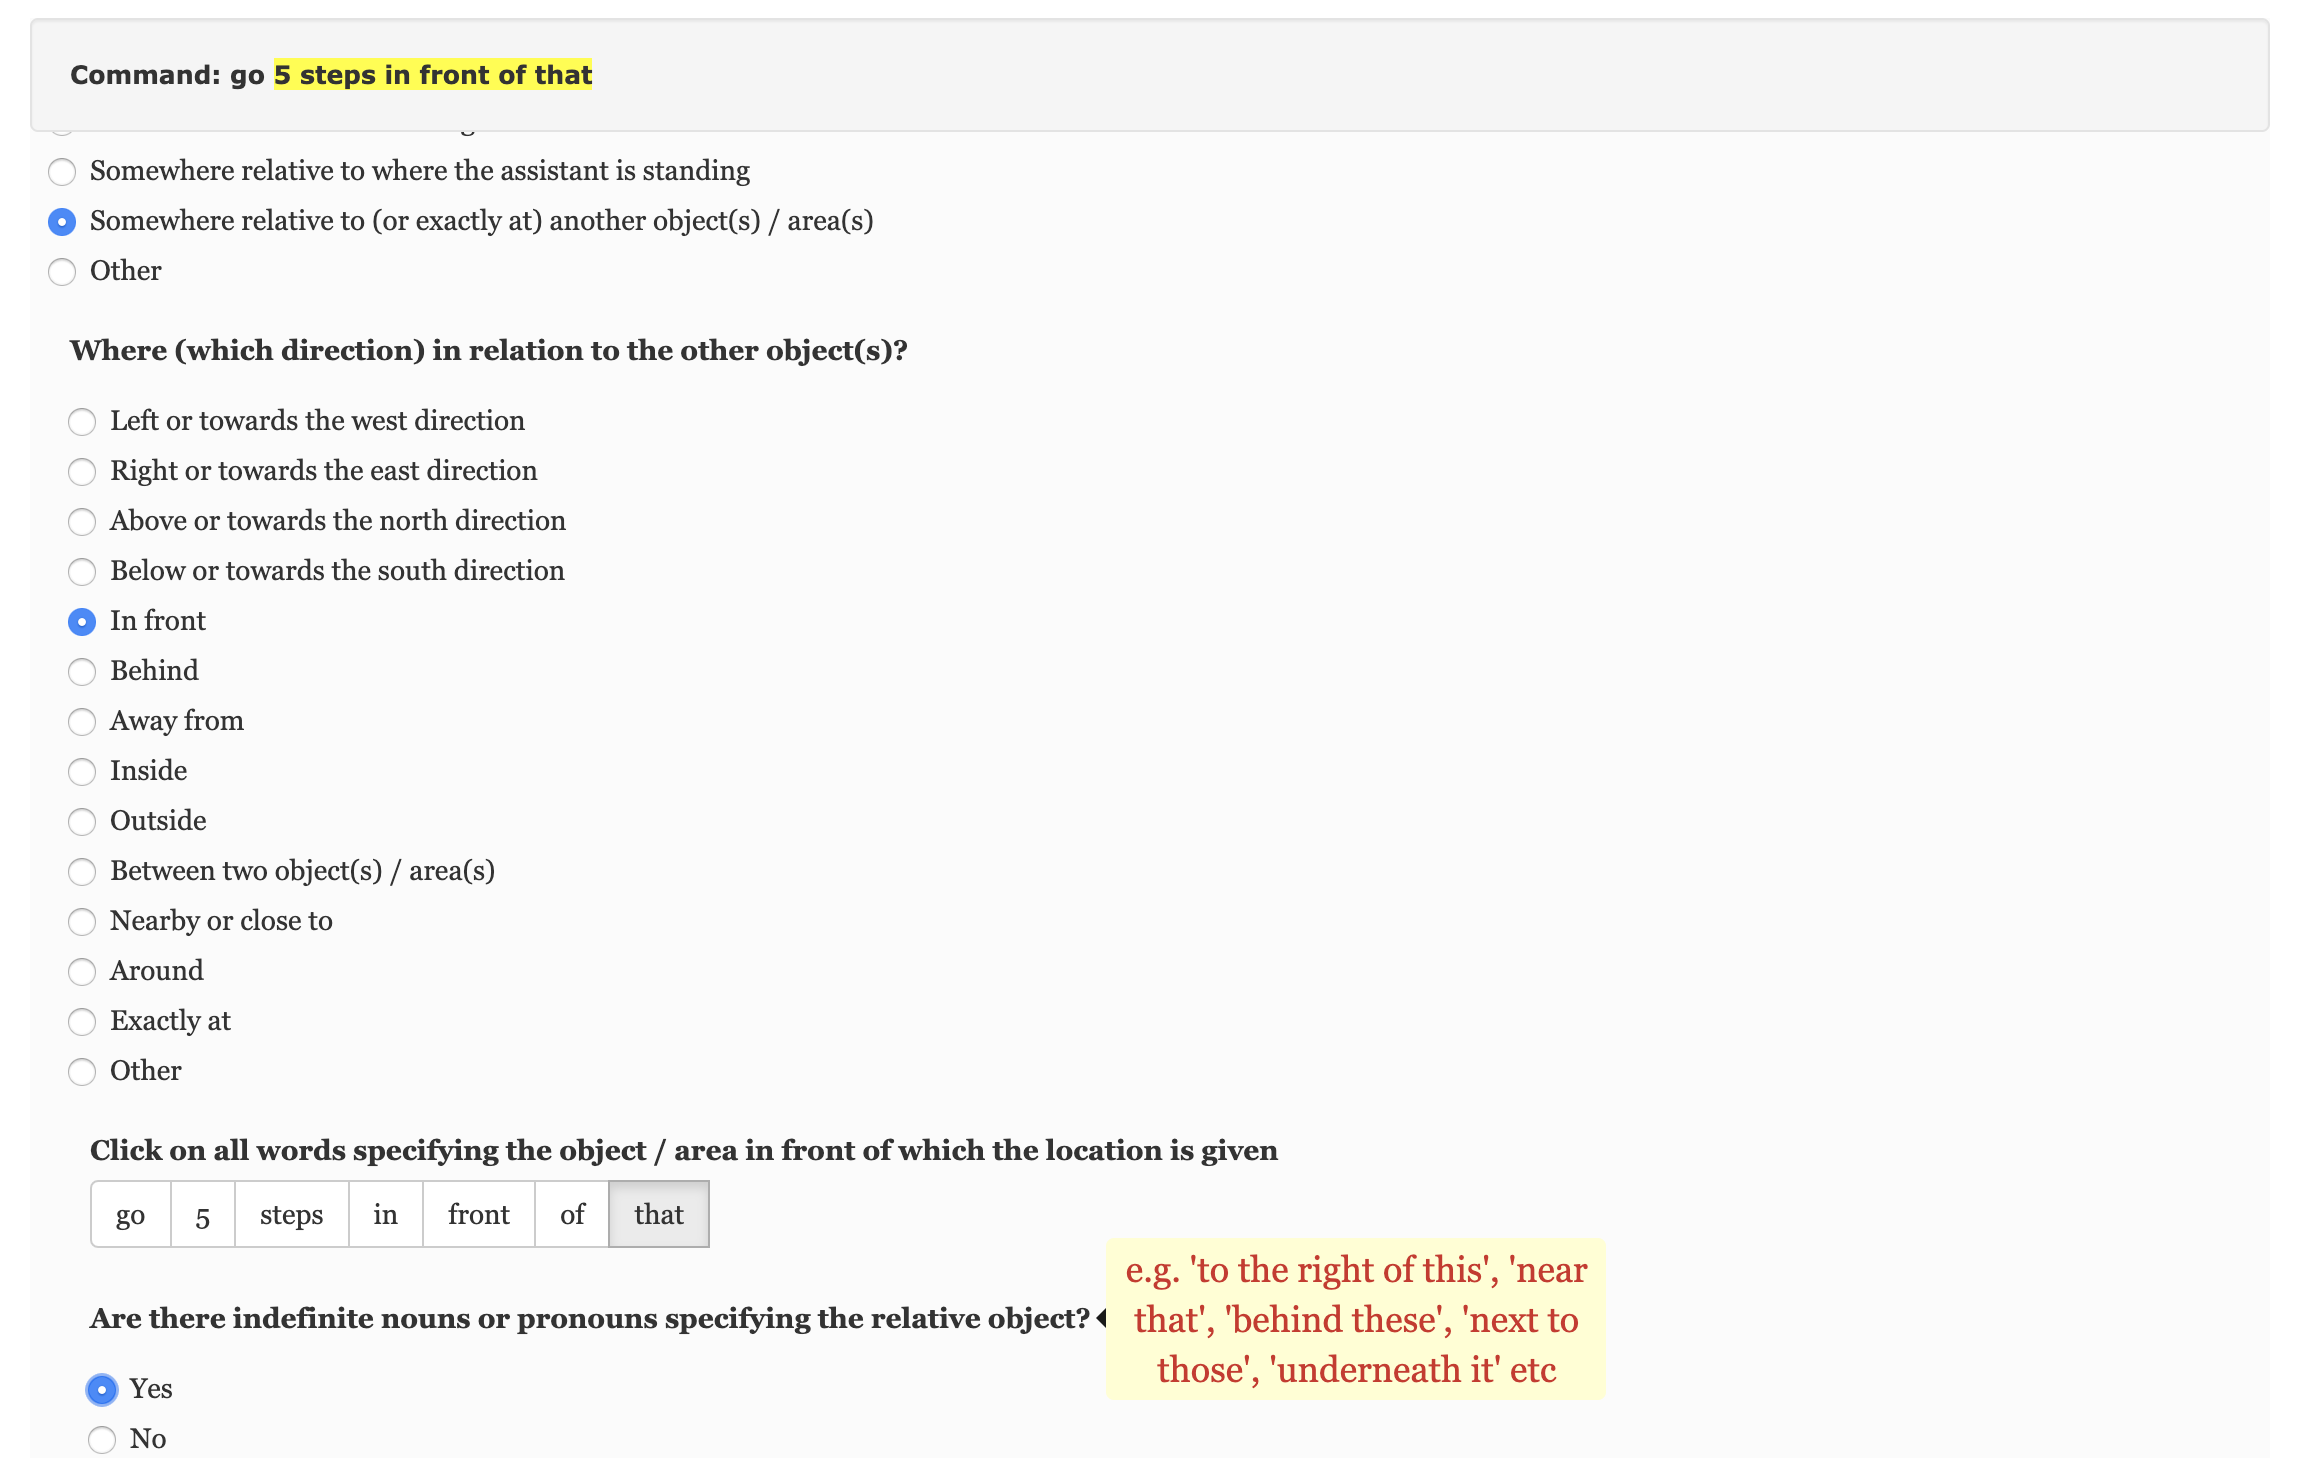
\includegraphics[width=\linewidth, height=6cm, ,keepaspectratio  ]{figures/23.png} 
     \bigbreak
     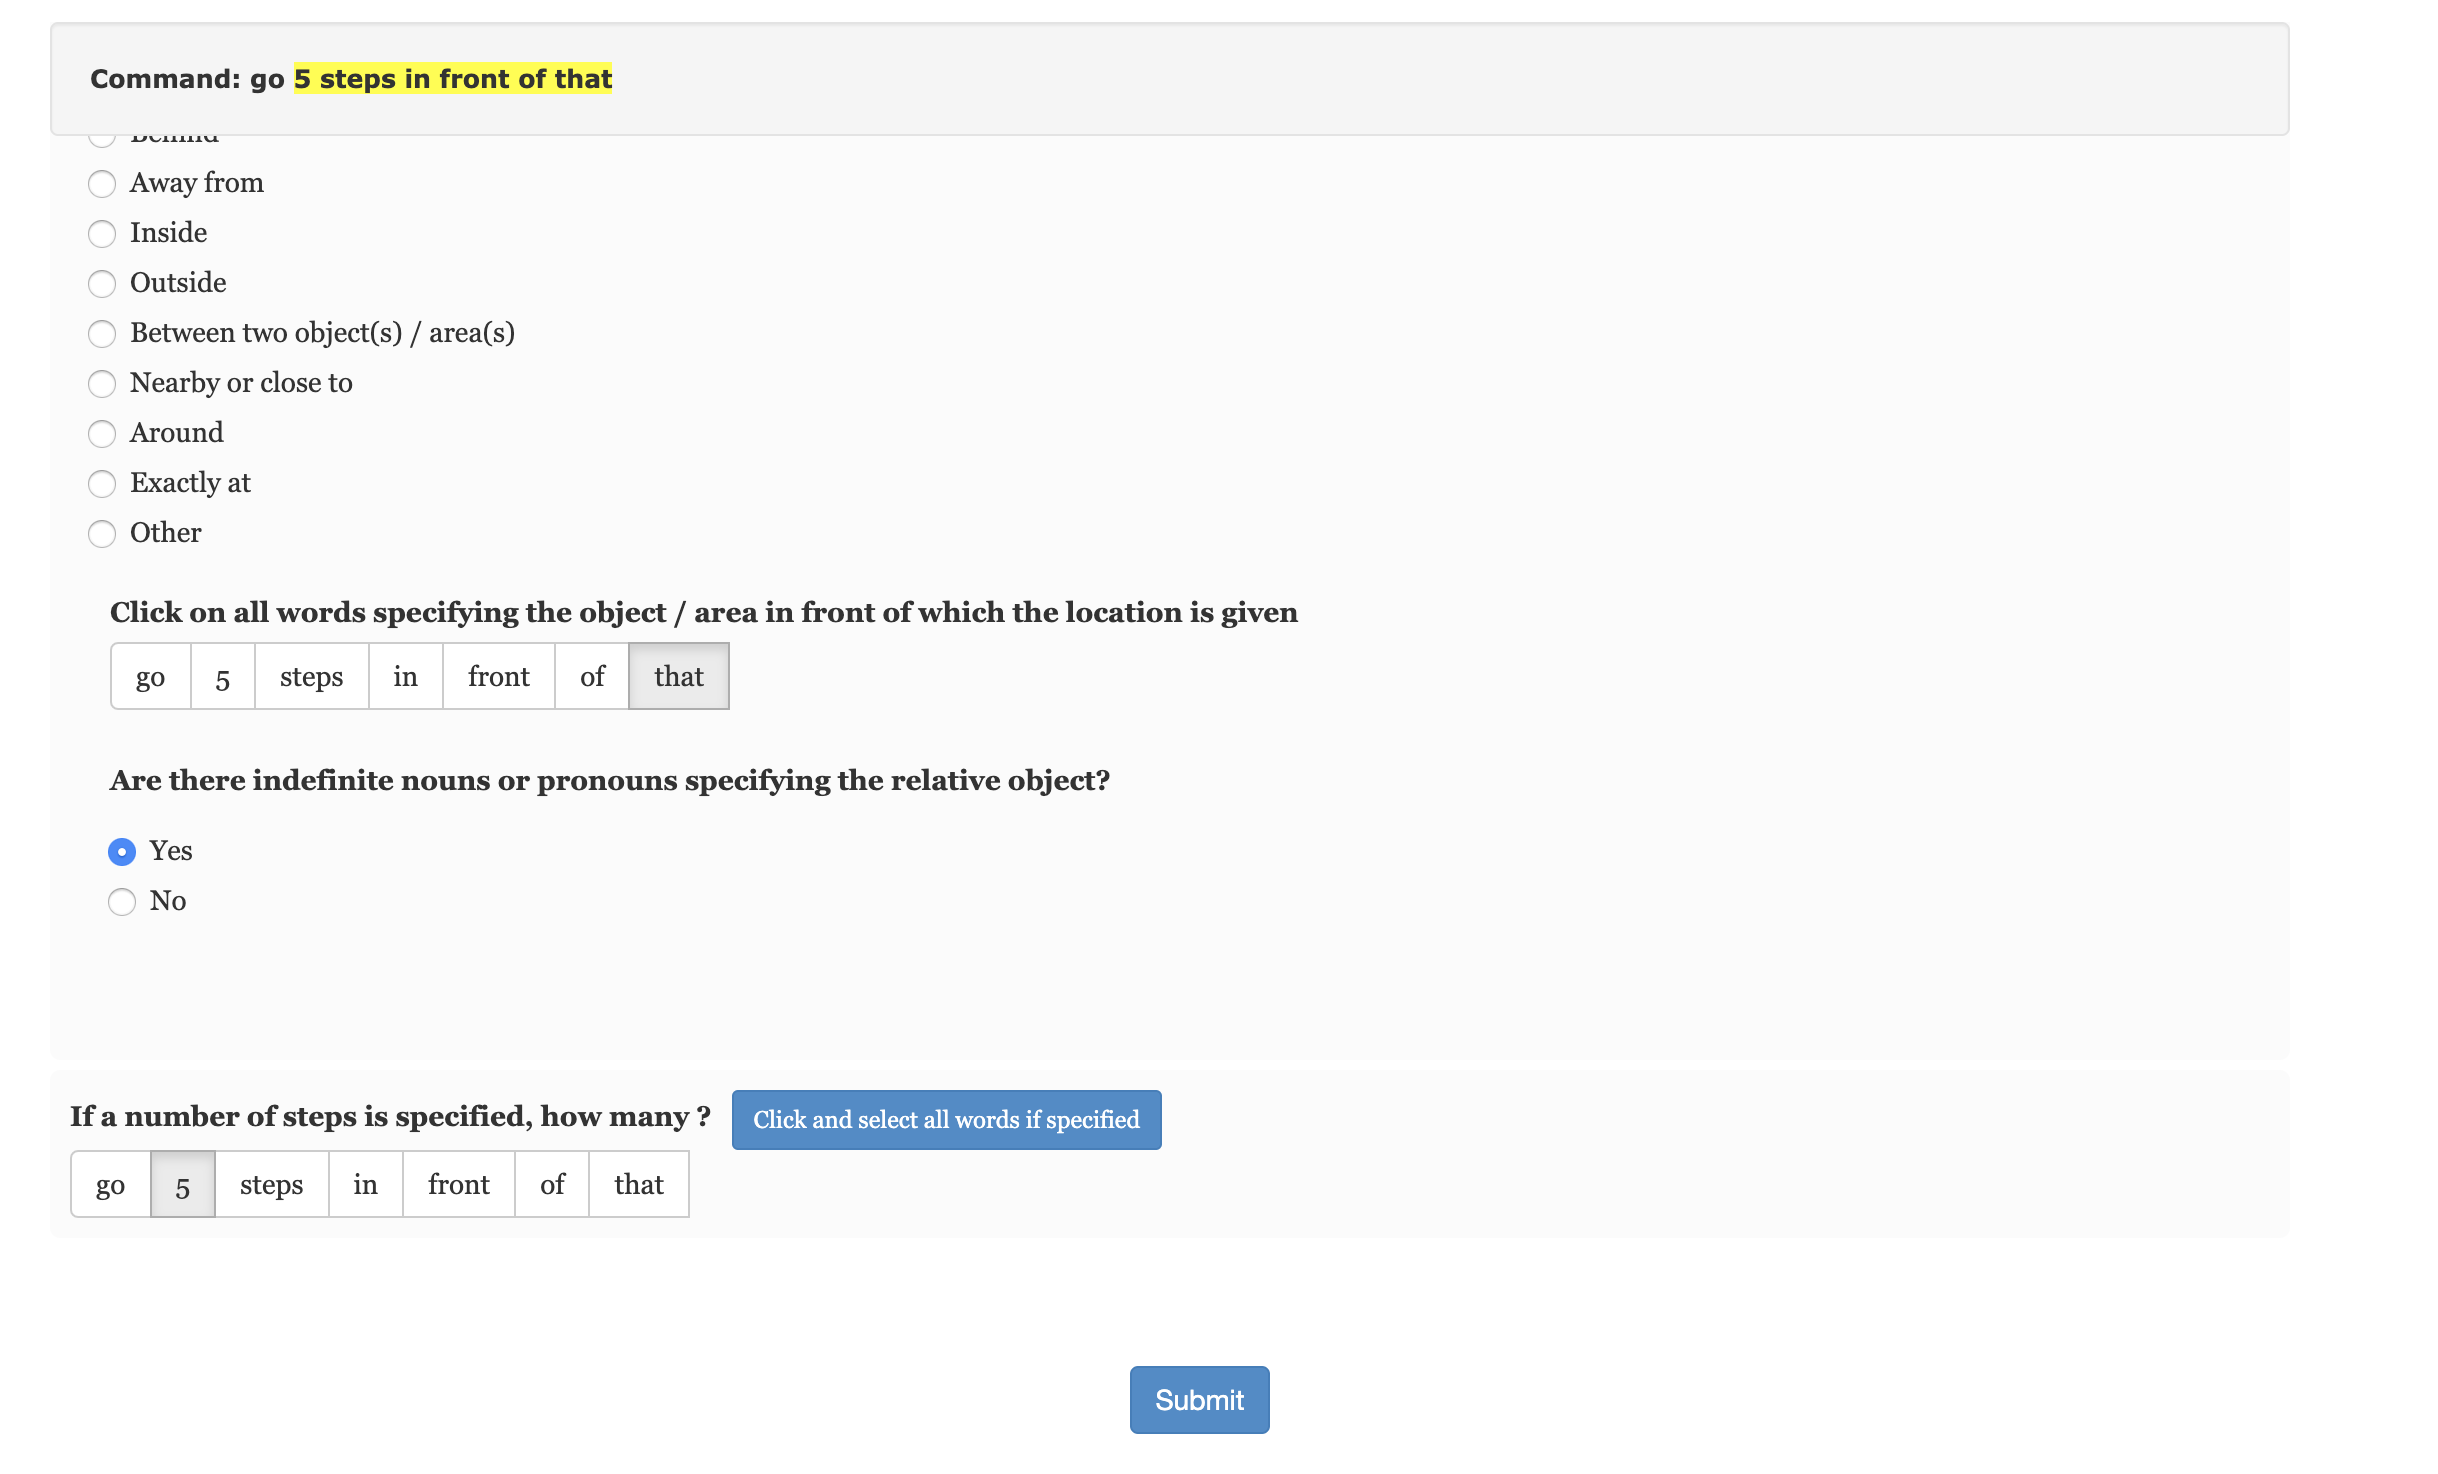
\includegraphics[width=0.65\linewidth, height=6cm, keepaspectratio ]{figures/24.png}
	 \caption{The step by step screenshot of annotating properties of highlighted words for``location''  in a ``Move'' action.}
	\label{fig:move_location}
\end{figure}

\begin{figure}[h]
    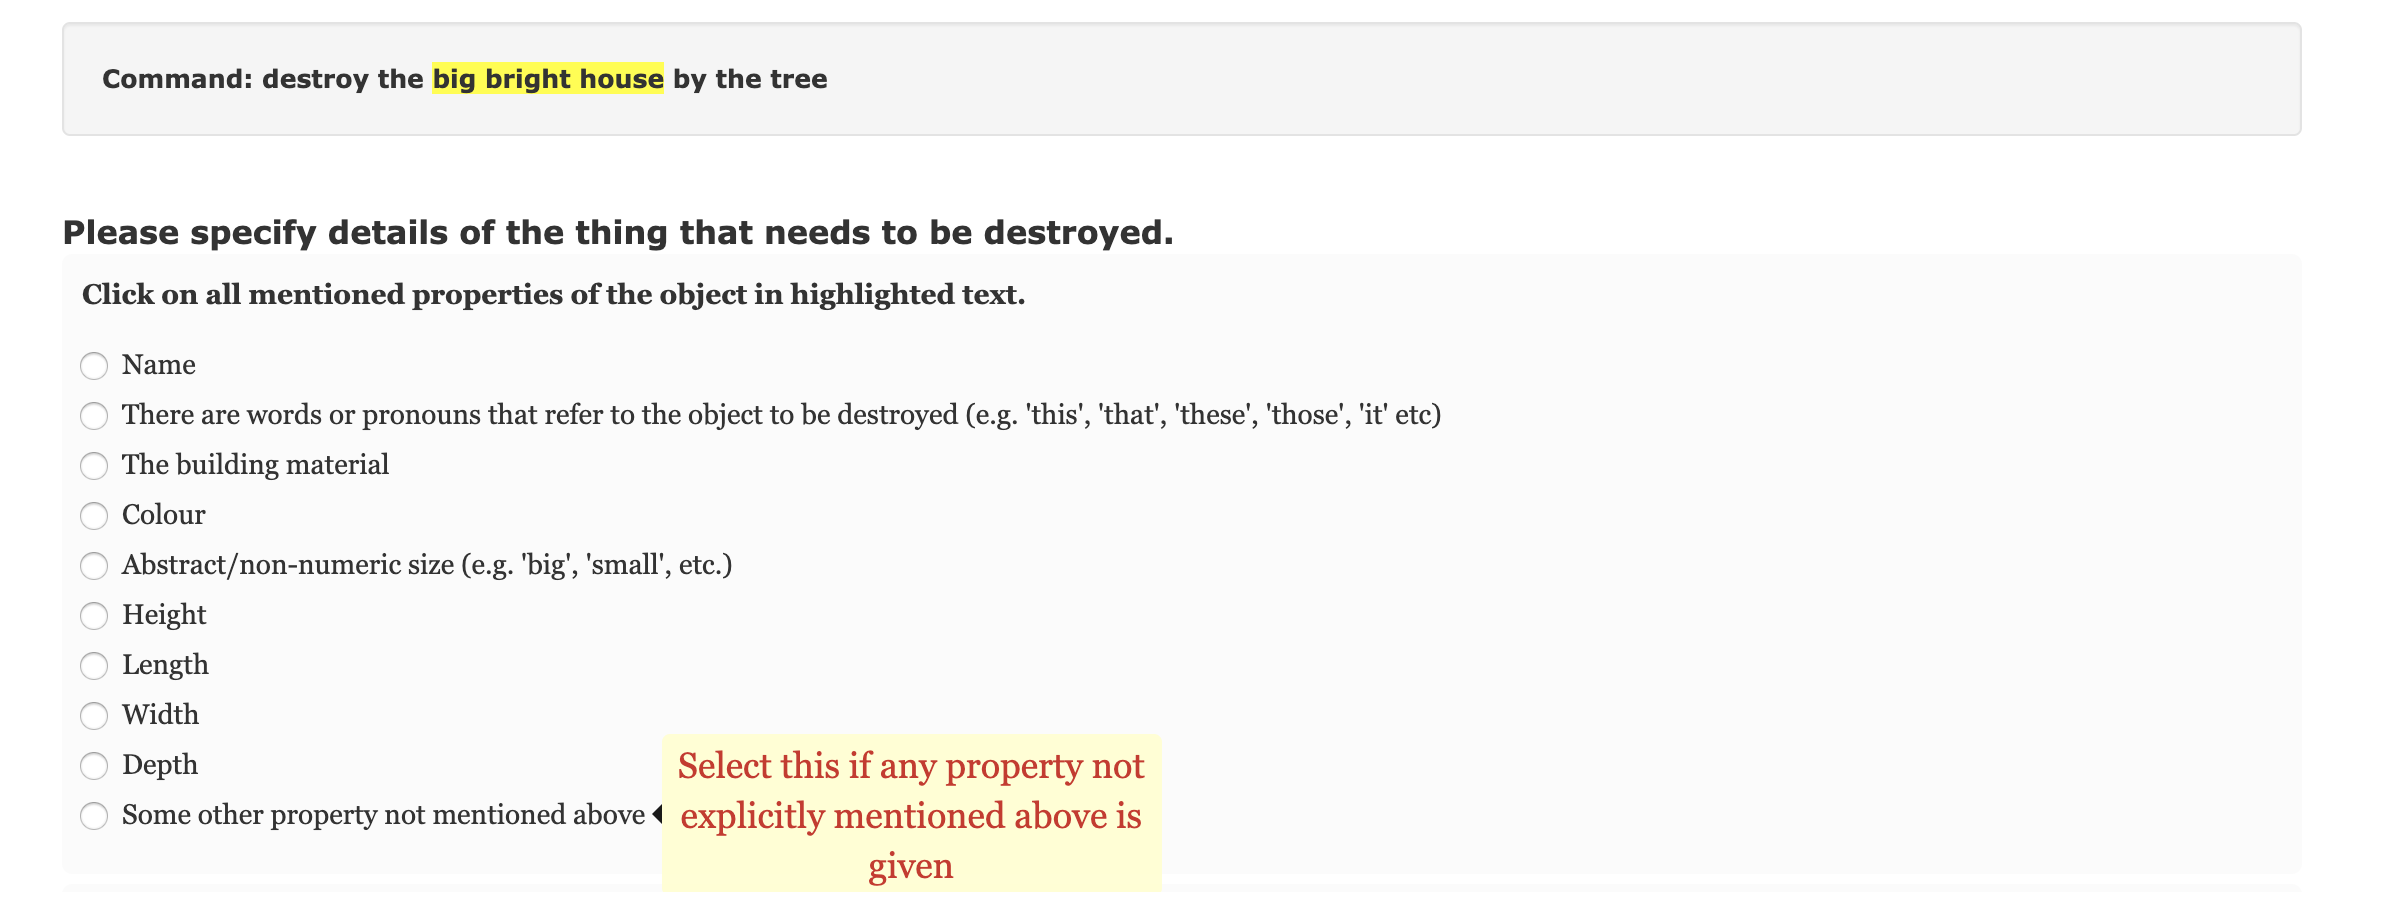
\includegraphics[width=0.70\linewidth, height=6cm, ,keepaspectratio  ]{figures/25.png}
    \bigbreak
     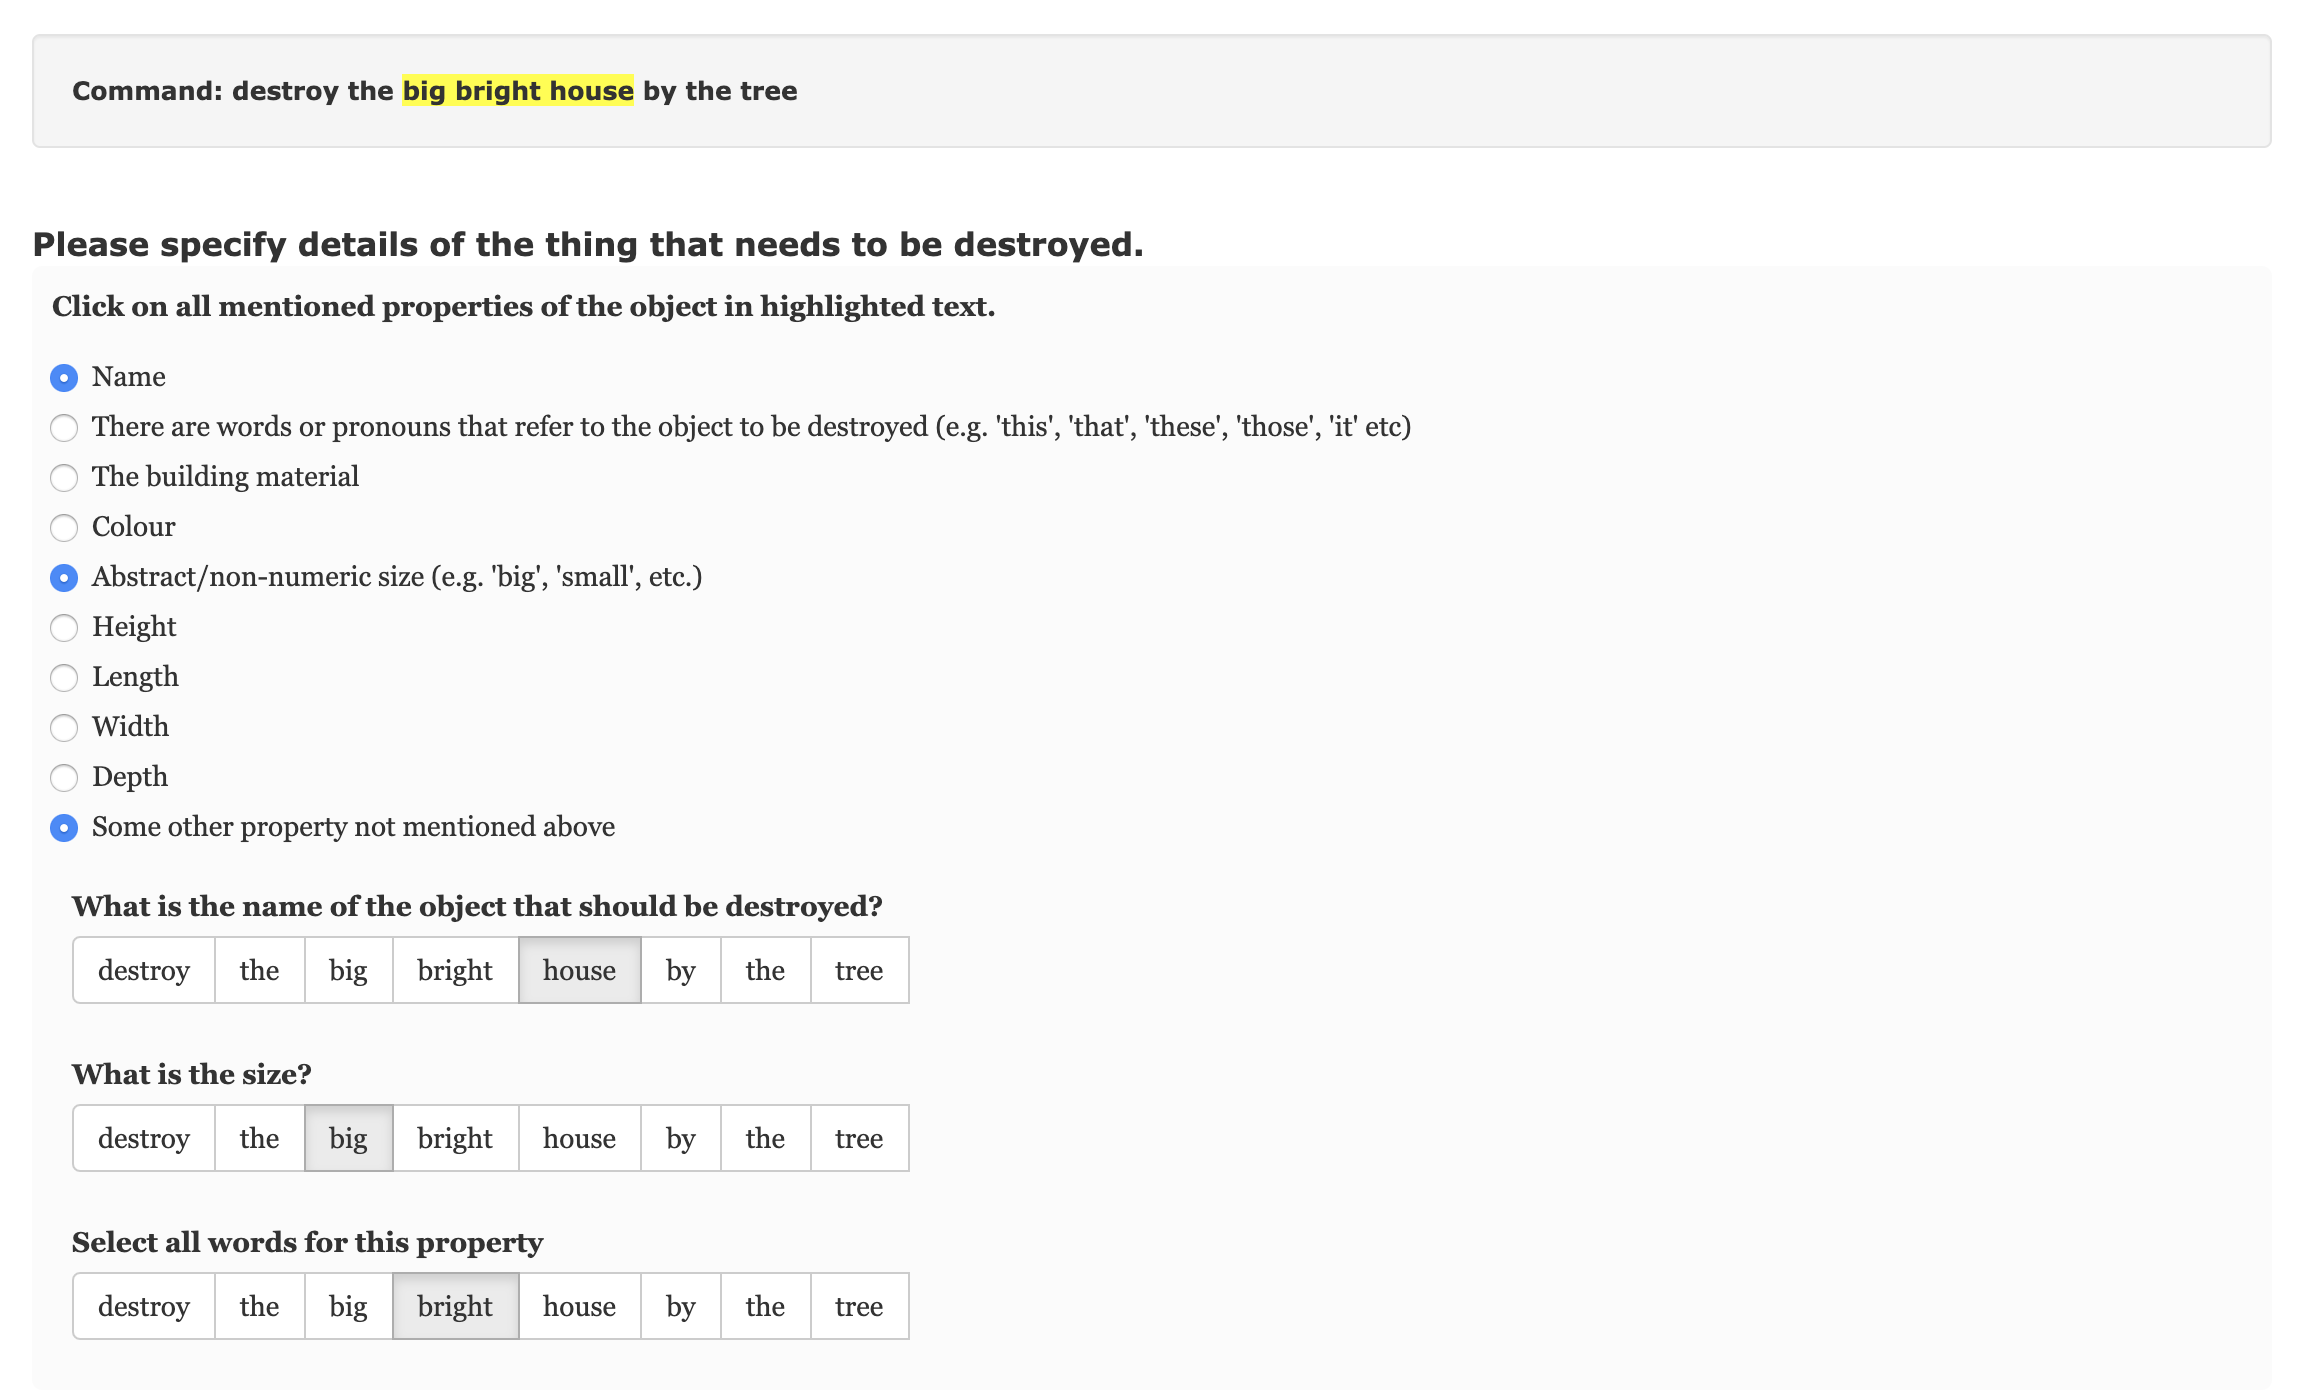
\includegraphics[width=\linewidth, height=6cm, ,keepaspectratio  ]{figures/26.png} 
	 \caption{The step by step screenshot of annotating properties of highlighted words for``reference\_object''  in a ``Destroy'' action.}
	\label{fig:destroy_ref}
\end{figure}

\subsection{Tool for composite commands}
\label{sec:composite}
This tool is meant for ``composite'' commands (commands that include multiple actions) and asks the users to split a command into multiple individual commands. The instruction for this are shown in figure \ref{fig:comp}. Once we get the split, we send out each command to annotation tool described in Section \ref{sec:anntn}
\begin{figure}
	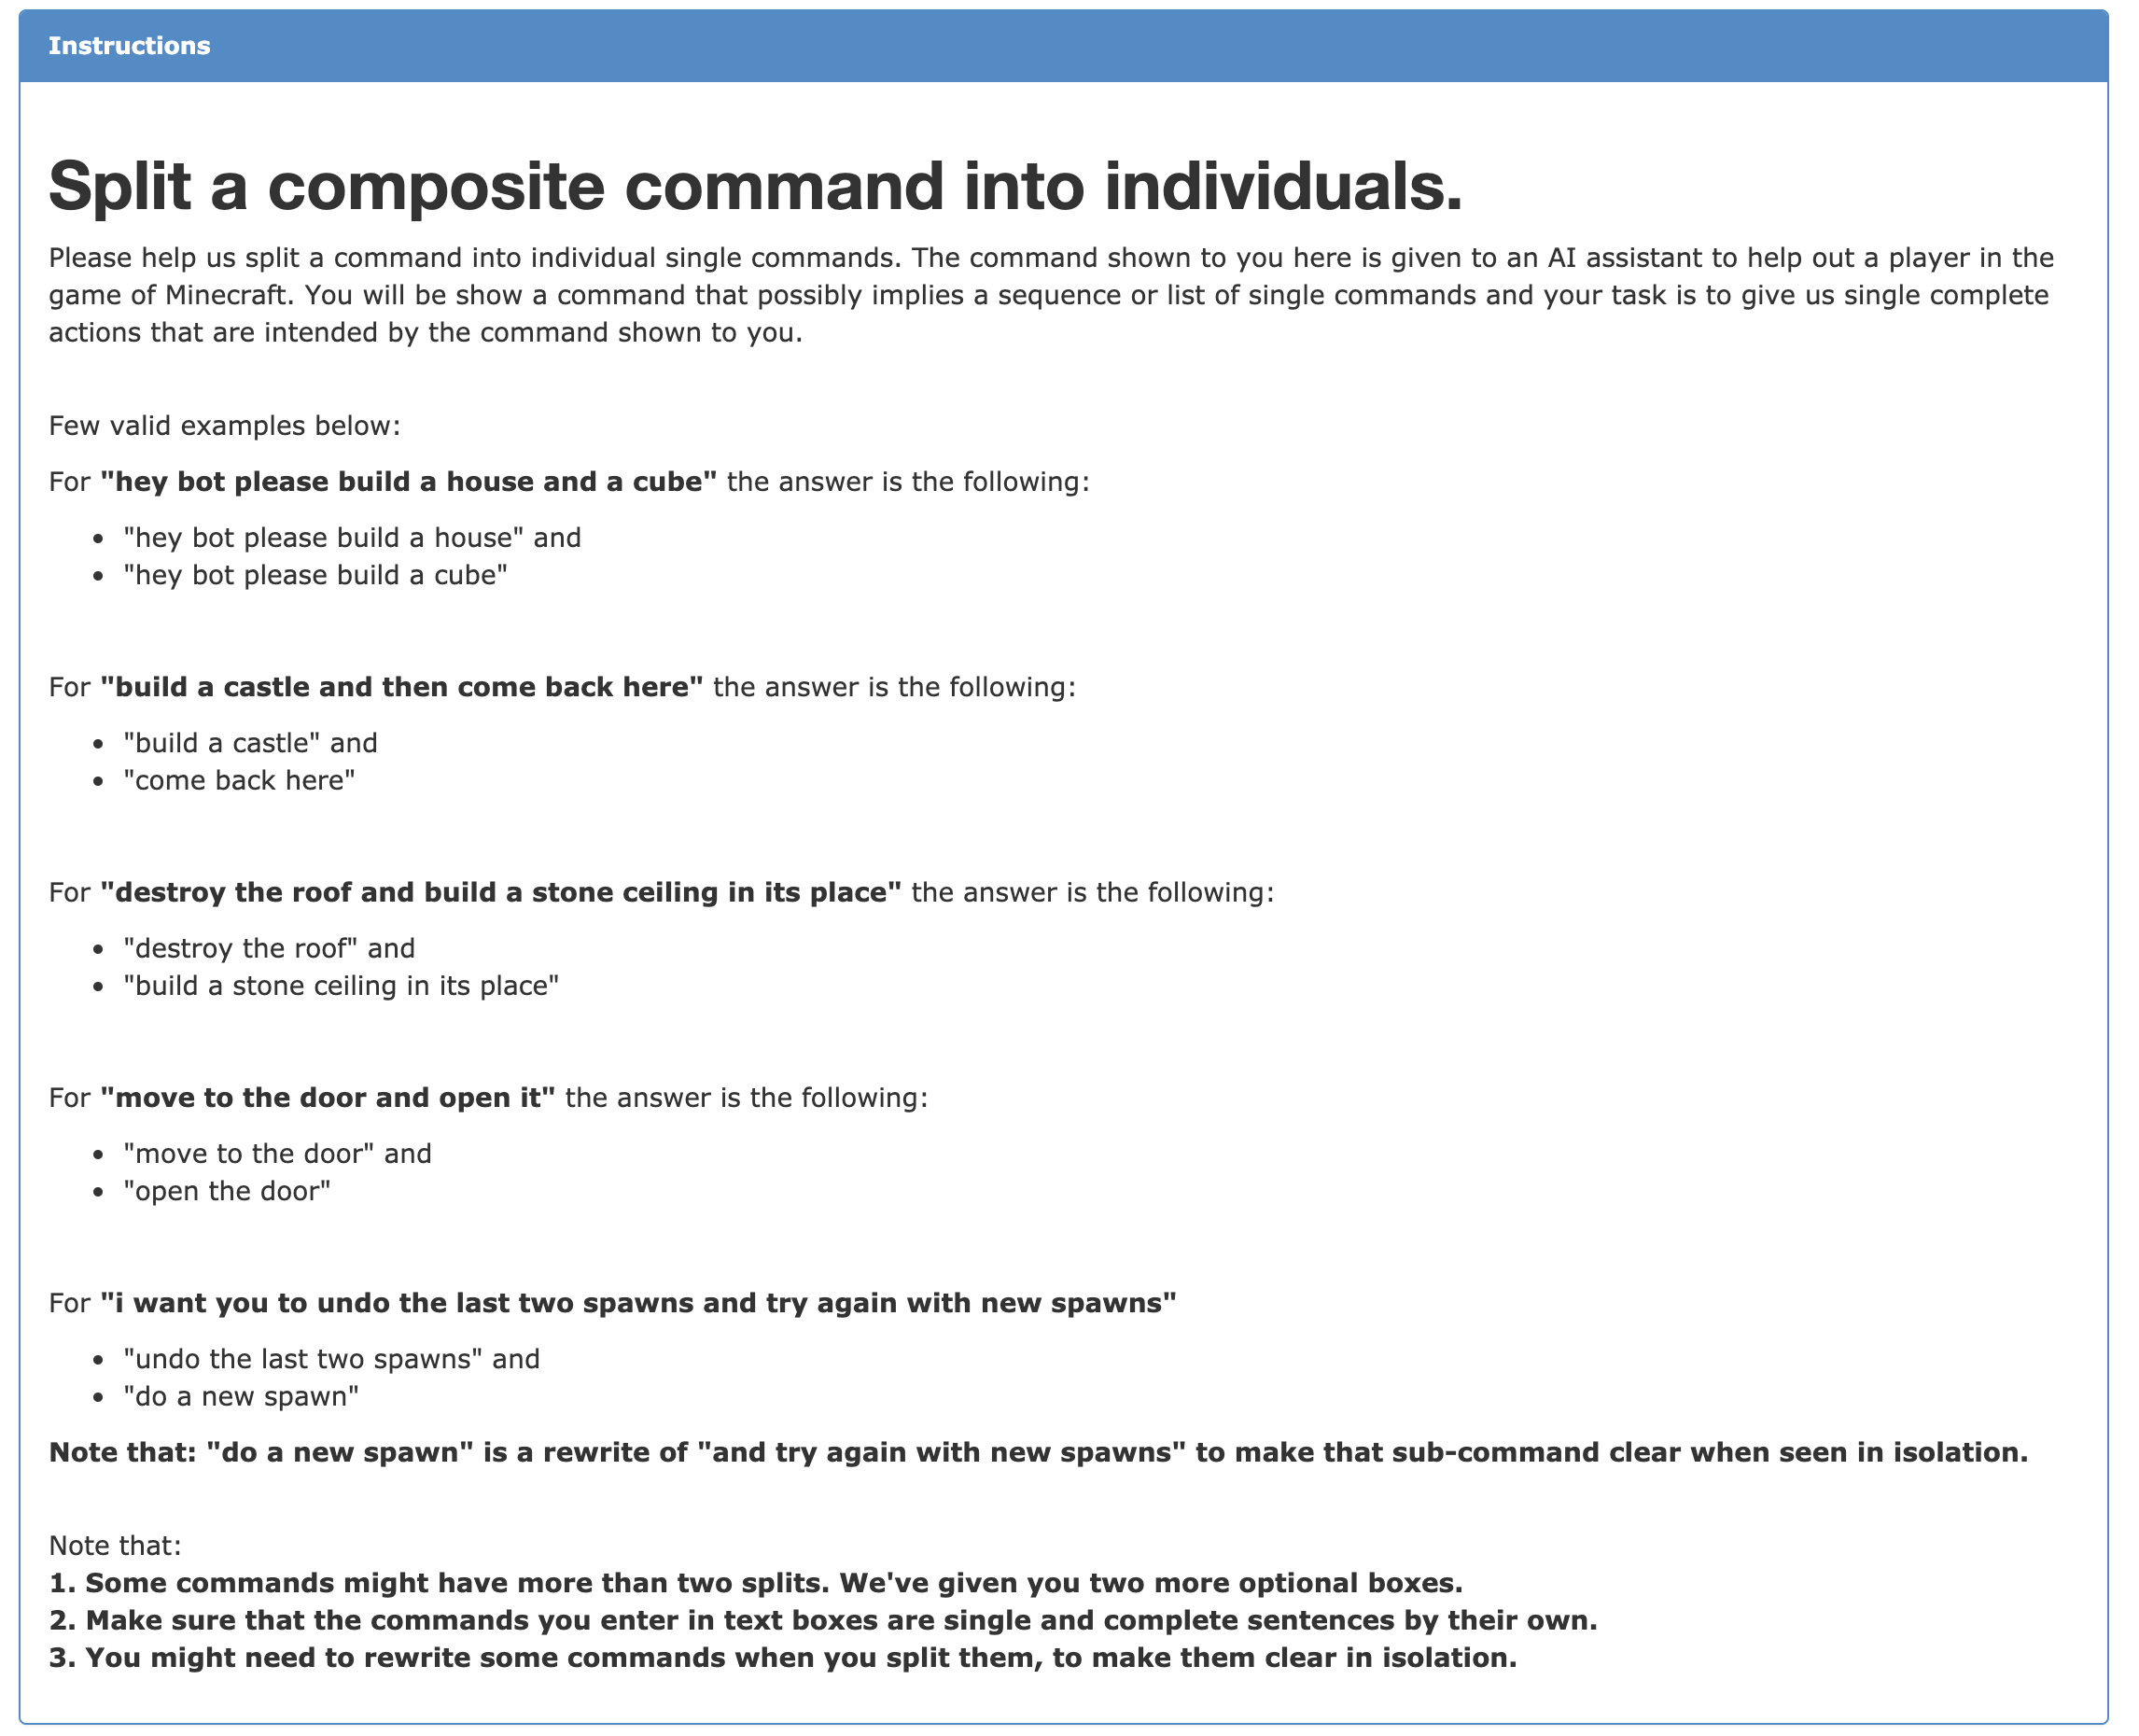
\includegraphics[width=\linewidth ]{figures/composite.png}
	\caption{The task instructions shown to crowd-sourced workers for splitting composite commands}
	\label{fig:comp}
\end{figure}

\clearpage
\onecolumn

\section{Action Tree structure}
\label{sec:action_tree}

%\begin{figure*}[ht!]
%    \centering
%     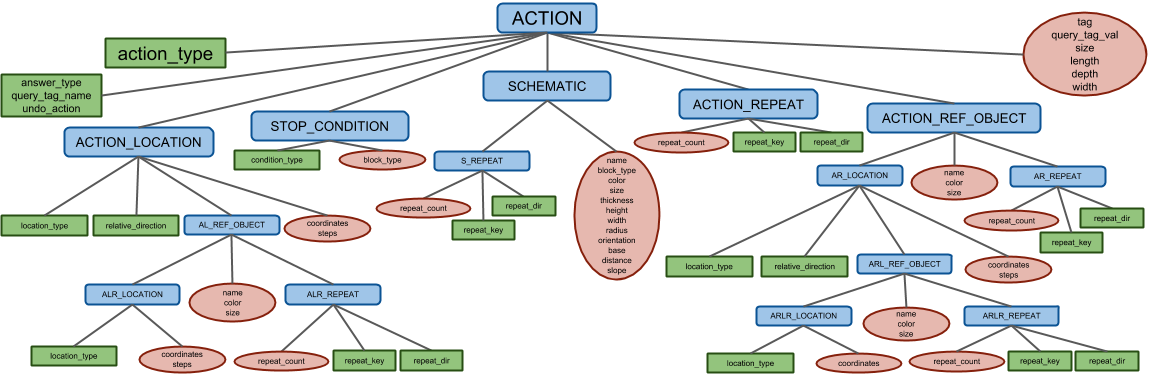
\includegraphics[natwidth=\linewidth]{figures/ActionGrammar.png}
%    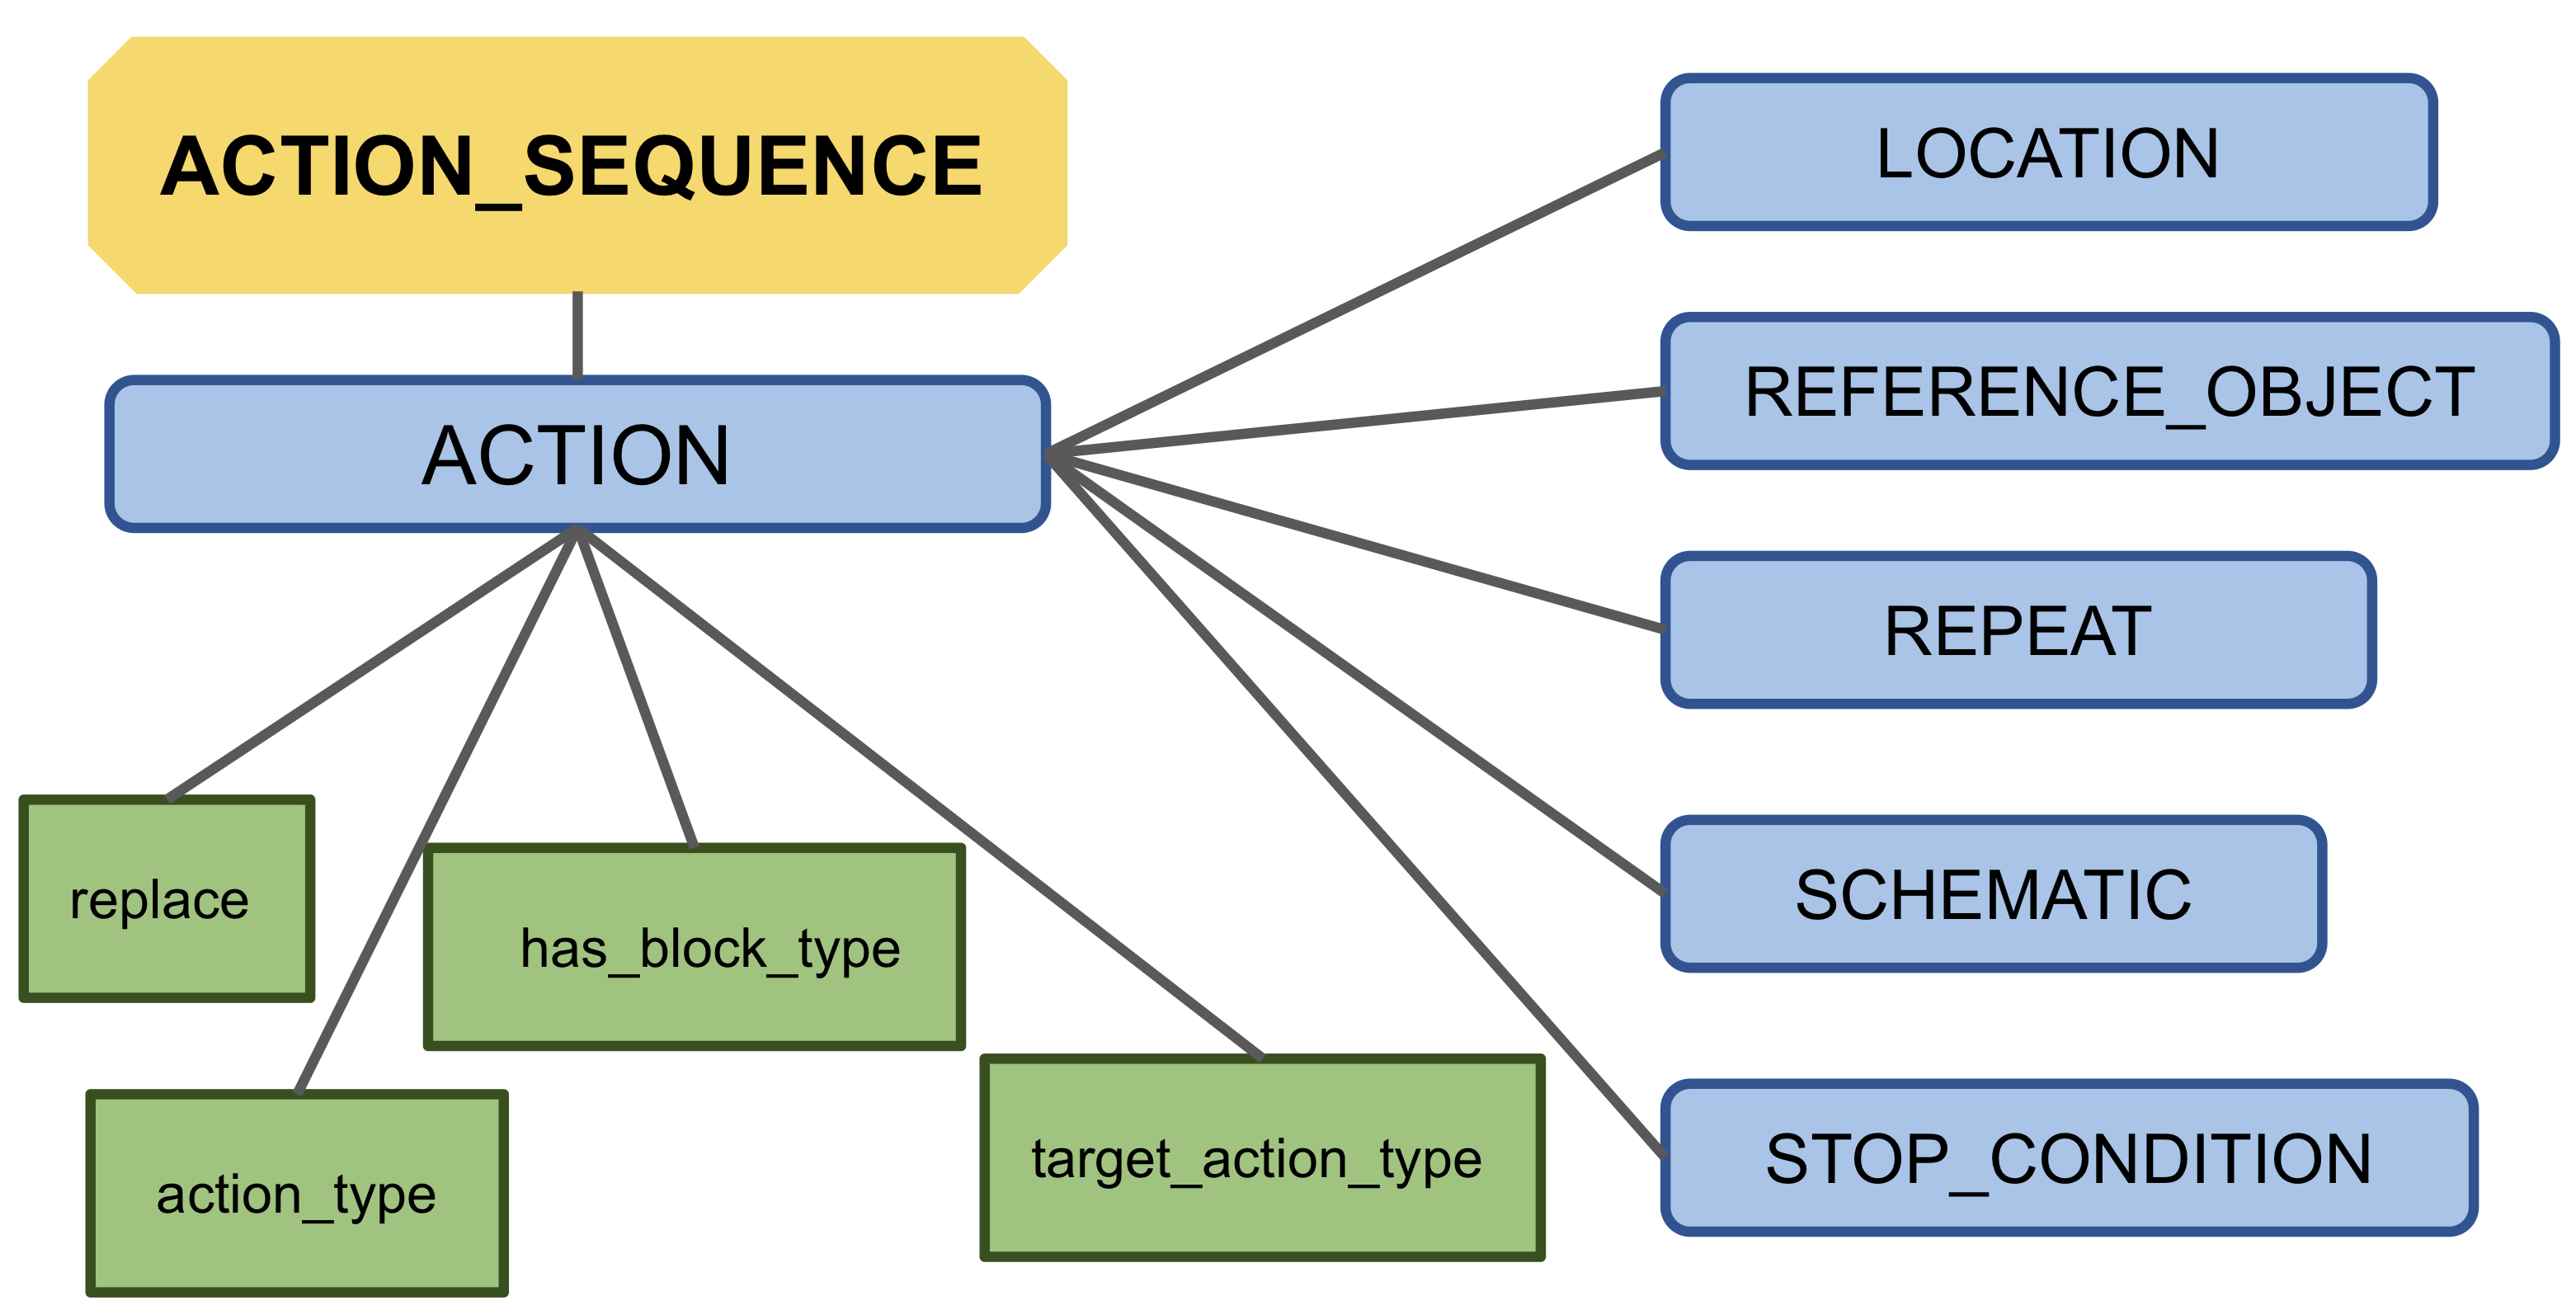
\includegraphics[width=0.70\linewidth]{figures/AS.png}
%    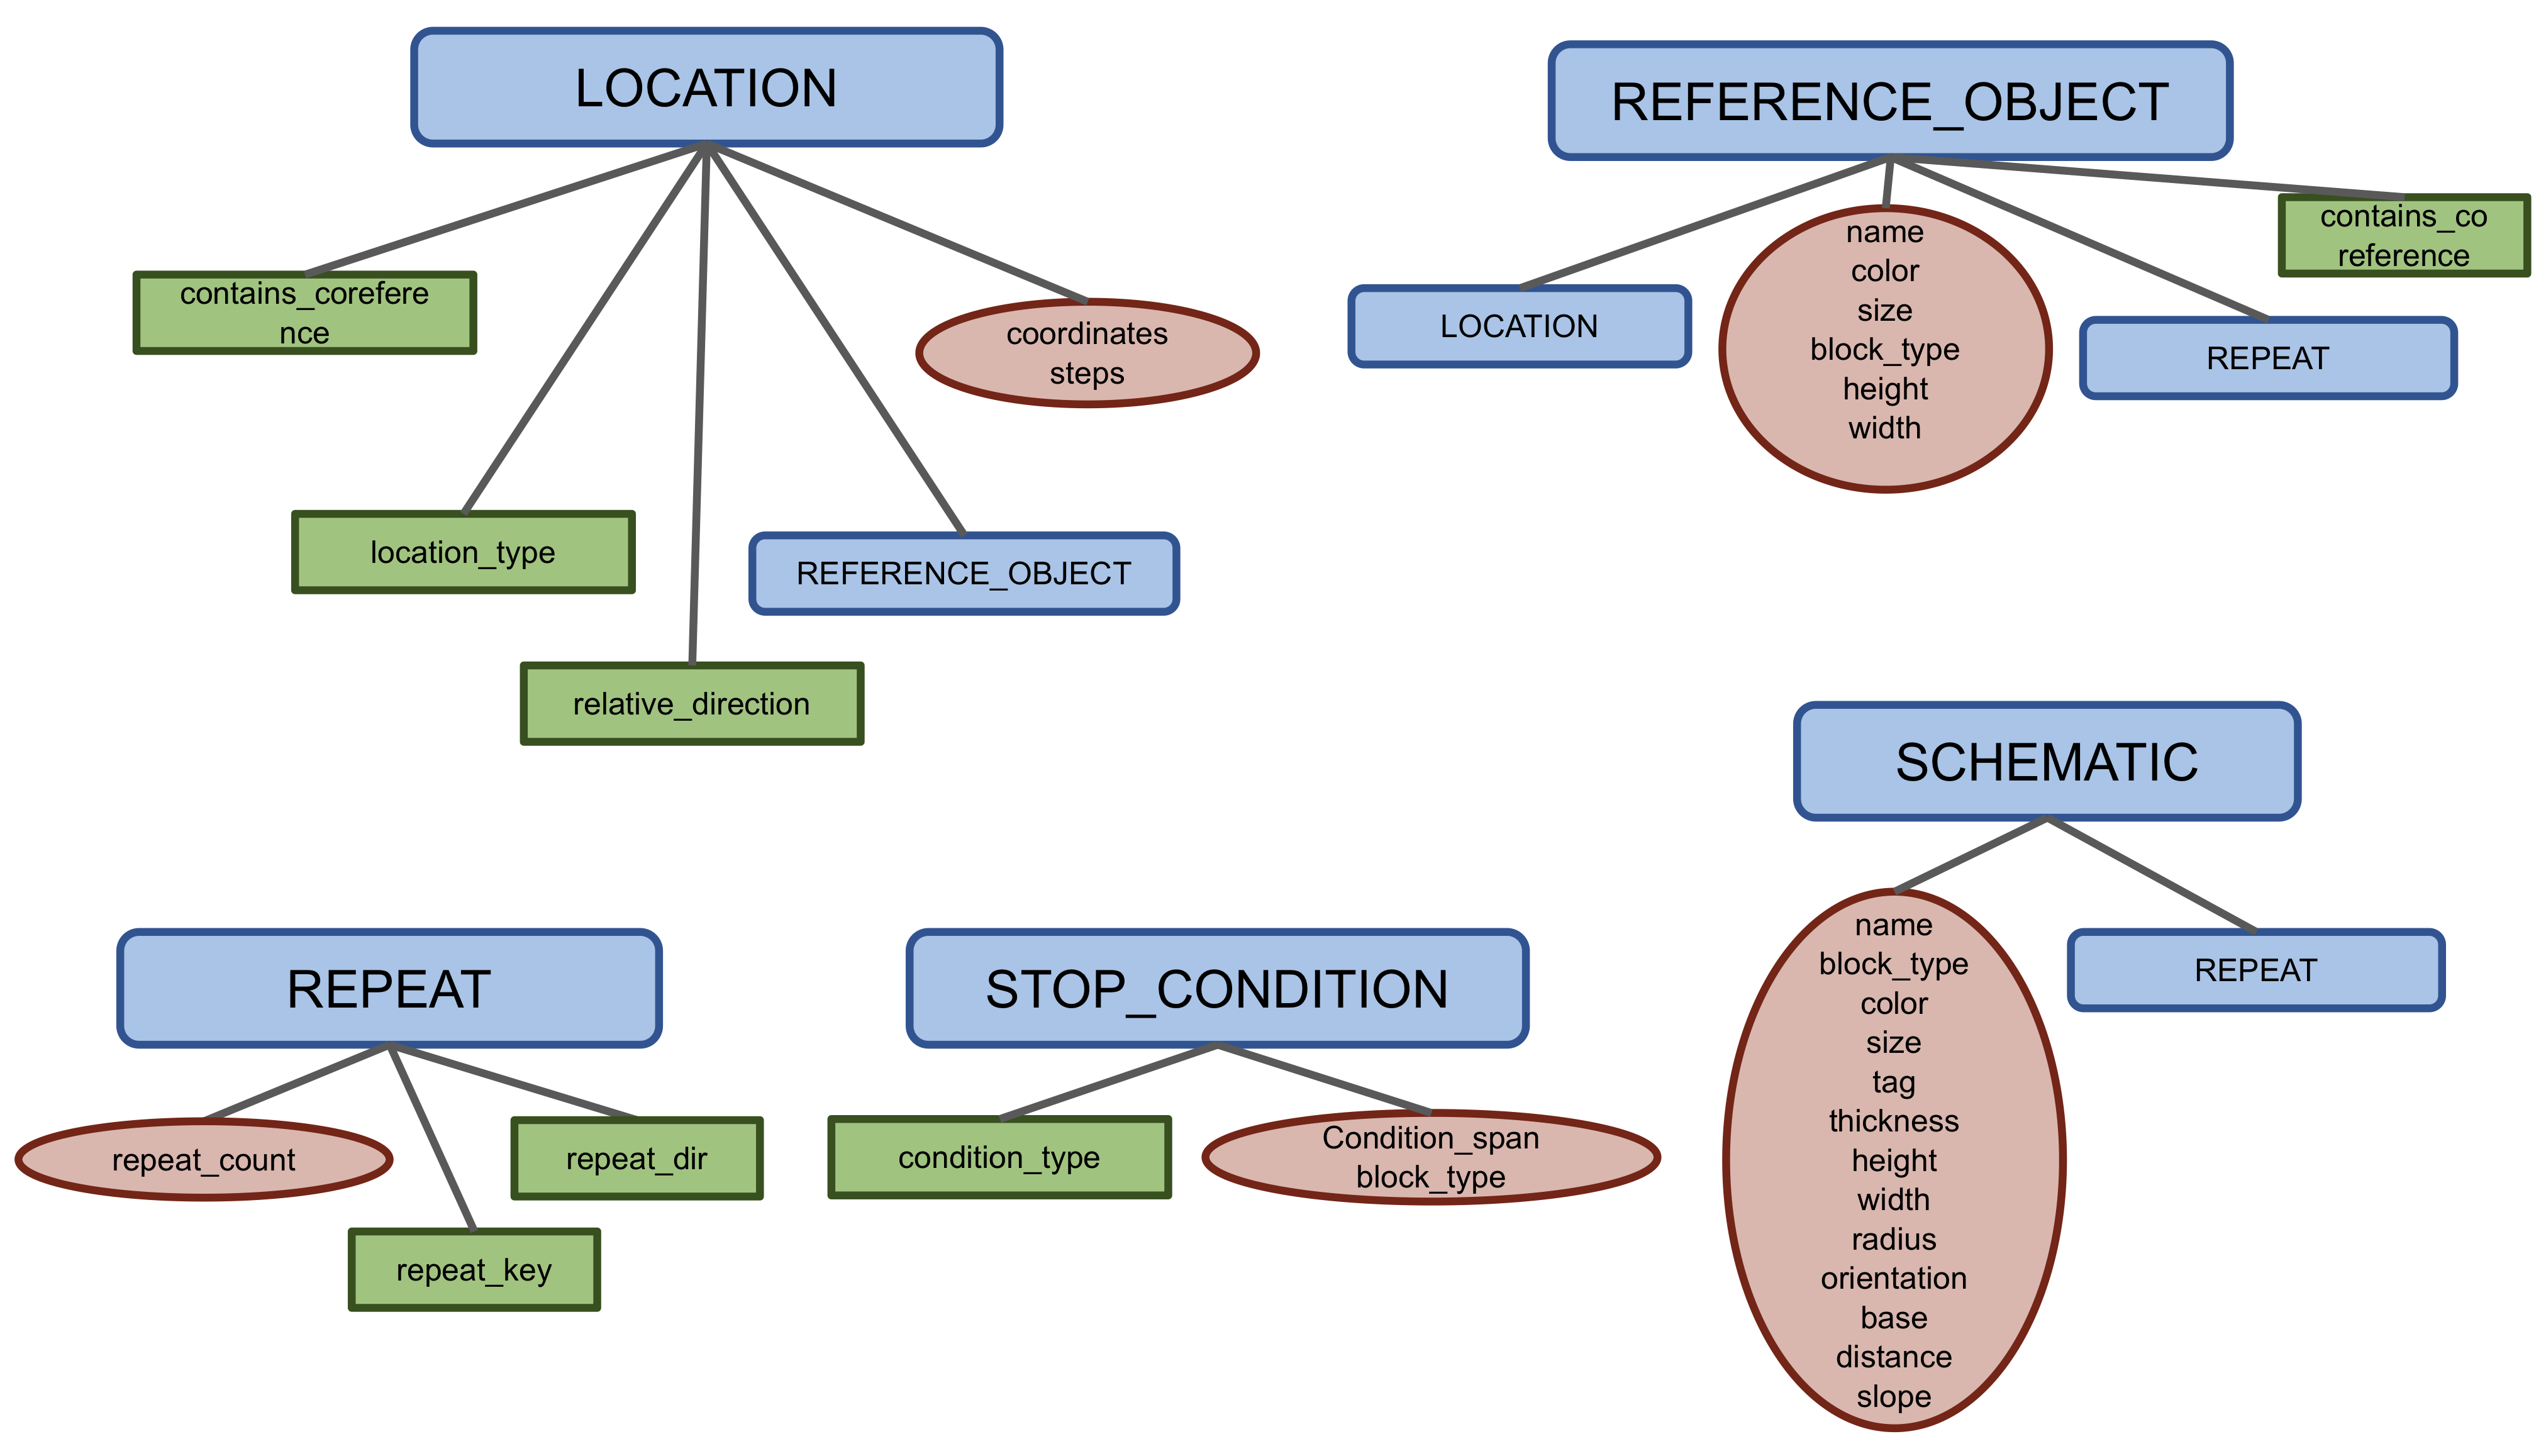
\includegraphics[width=0.30\linewidth]{figures/NOT_AS.png}
%    \caption{Action space grammar}
%    \label{fig:action_grammar}
%\end{figure*}
This section describes the details of logical form of each action.
We support three dialogue types: HUMAN\_GIVE\_COMMAND, GET\_MEMORY and PUT\_MEMORY.
The logical form for actions has been pictorially represented in Figures: \ref{fig:AS} and \ref{fig:NOT_AS}

We support the following actions in our dataset : Build, Copy, Dance, Spawn, Resume, Fill, Destroy, Move, Undo, Stop, Dig and FreeBuild.
A lot of the actions use  ``location'' and ``reference\_object'' as children in their logical forms. To make the logical forms more presentable, we have shown the detailed representation of a ``reference\_object'' (reused in action trees using the variable: ``REF\_OBJECT'') in Figure \ref{fig:ref_obj} and the representation of ``location'' (reused in action trees using the variable: ``LOCATION'') in figure \ref{fig:location}. The representations of actions refer to these variable names in their trees.


\begin{figure}[h]
    \centering
    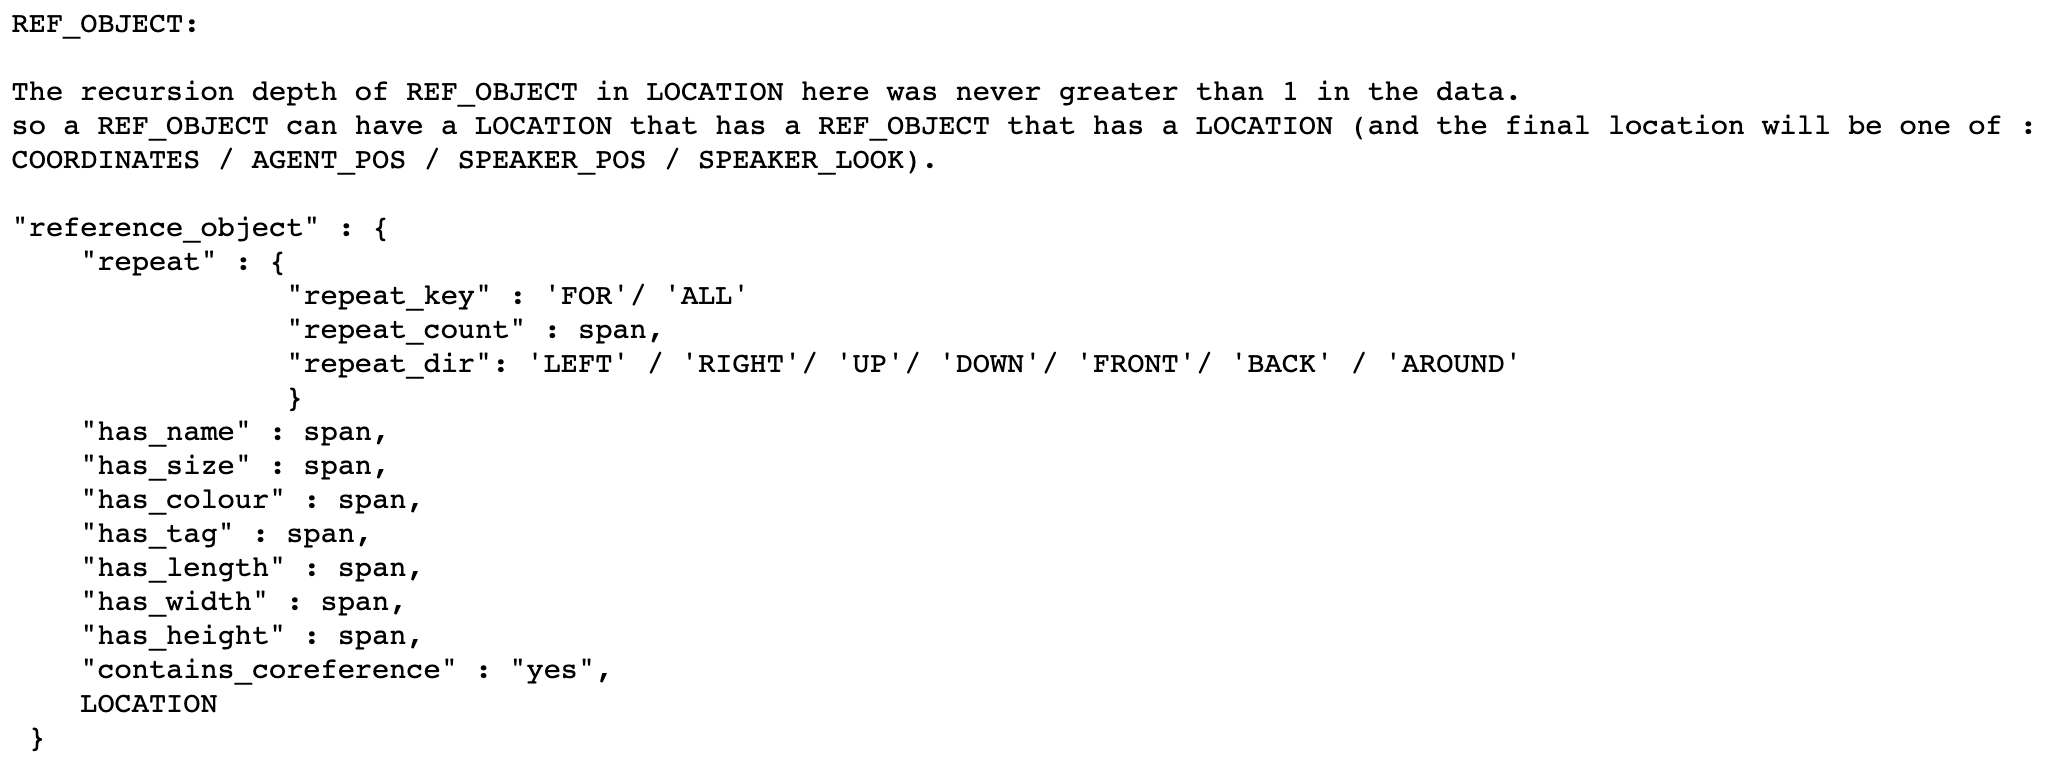
\includegraphics[width=15cm,height=20cm,keepaspectratio]{figures/ref_obj.png}
    \caption{Logical form of a reference\_object child}
    \label{fig:ref_obj}
\end{figure}


\begin{figure}[h]
    \centering
    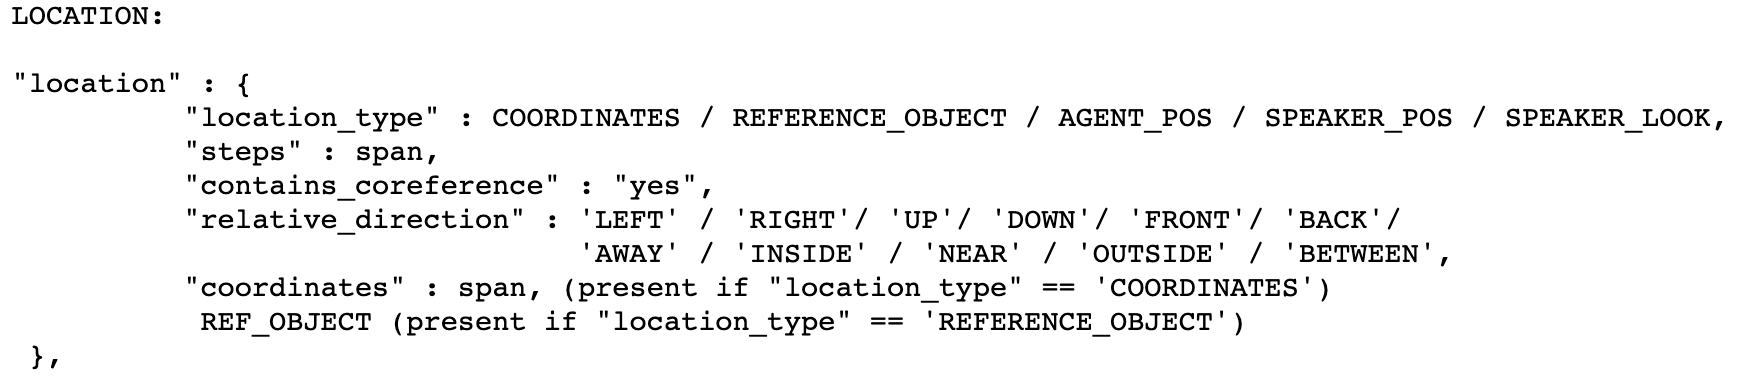
\includegraphics[width=15cm,height=20cm,keepaspectratio]{figures/location.png}
    \caption{Logical form of a location child}
    \label{fig:location}
\end{figure}
The detailed action tree for each action and dialogue type has been presented in the following subsections. Figure~\ref{fig:action_tree_ex} shows an example for a \textsc{build} action.

\begin{figure}[ht]
    \centering
    \small
    \begin{verbatim}
  0     1    2   3     4    5   6
"Make three oak wood houses to the
 7   8   9   10   11    12
left of the dark grey church."


{"dialogue_type" : "HUMAN_GIVE_COMMAND",
 "action_sequence" : [
   {
    "action_type" : "BUILD",
    "schematic": {
      "has_block_type": [0, [2, 3]],
      "has_name": [0, [4, 4]],
      "repeat": {
        "repeat_key": "FOR",
        "repeat_count": [1, 1]
      }},
     "location": {
       "relative_direction": "LEFT",
       "location_type": "REFERENCE_OBJECT",
       "reference_object": {
         "has_colour_": [0, [10, 11]],
         "has_name_": [0, [12, 12]] }
}}]}
    \end{verbatim}
    \vspace{-20pt}
    \caption{An example logical form. The spans are indexed as : [sentence\_number, [starting\_word\_index, ending\_word\_index]].  sentence\_number is 0 for the most recent sentence spoken in a dialogue and is 0 in our dataset since we support one-turn dialogues as of now.}
    \vspace{-8pt}
    \label{fig:action_tree_ex}
\end{figure}


\subsection{ Build Action}
This is the action to Build a schematic at an optional location. The Build logical form is shown in \ref{fig:build_dict} .

\begin{figure}[h]
    \centering
    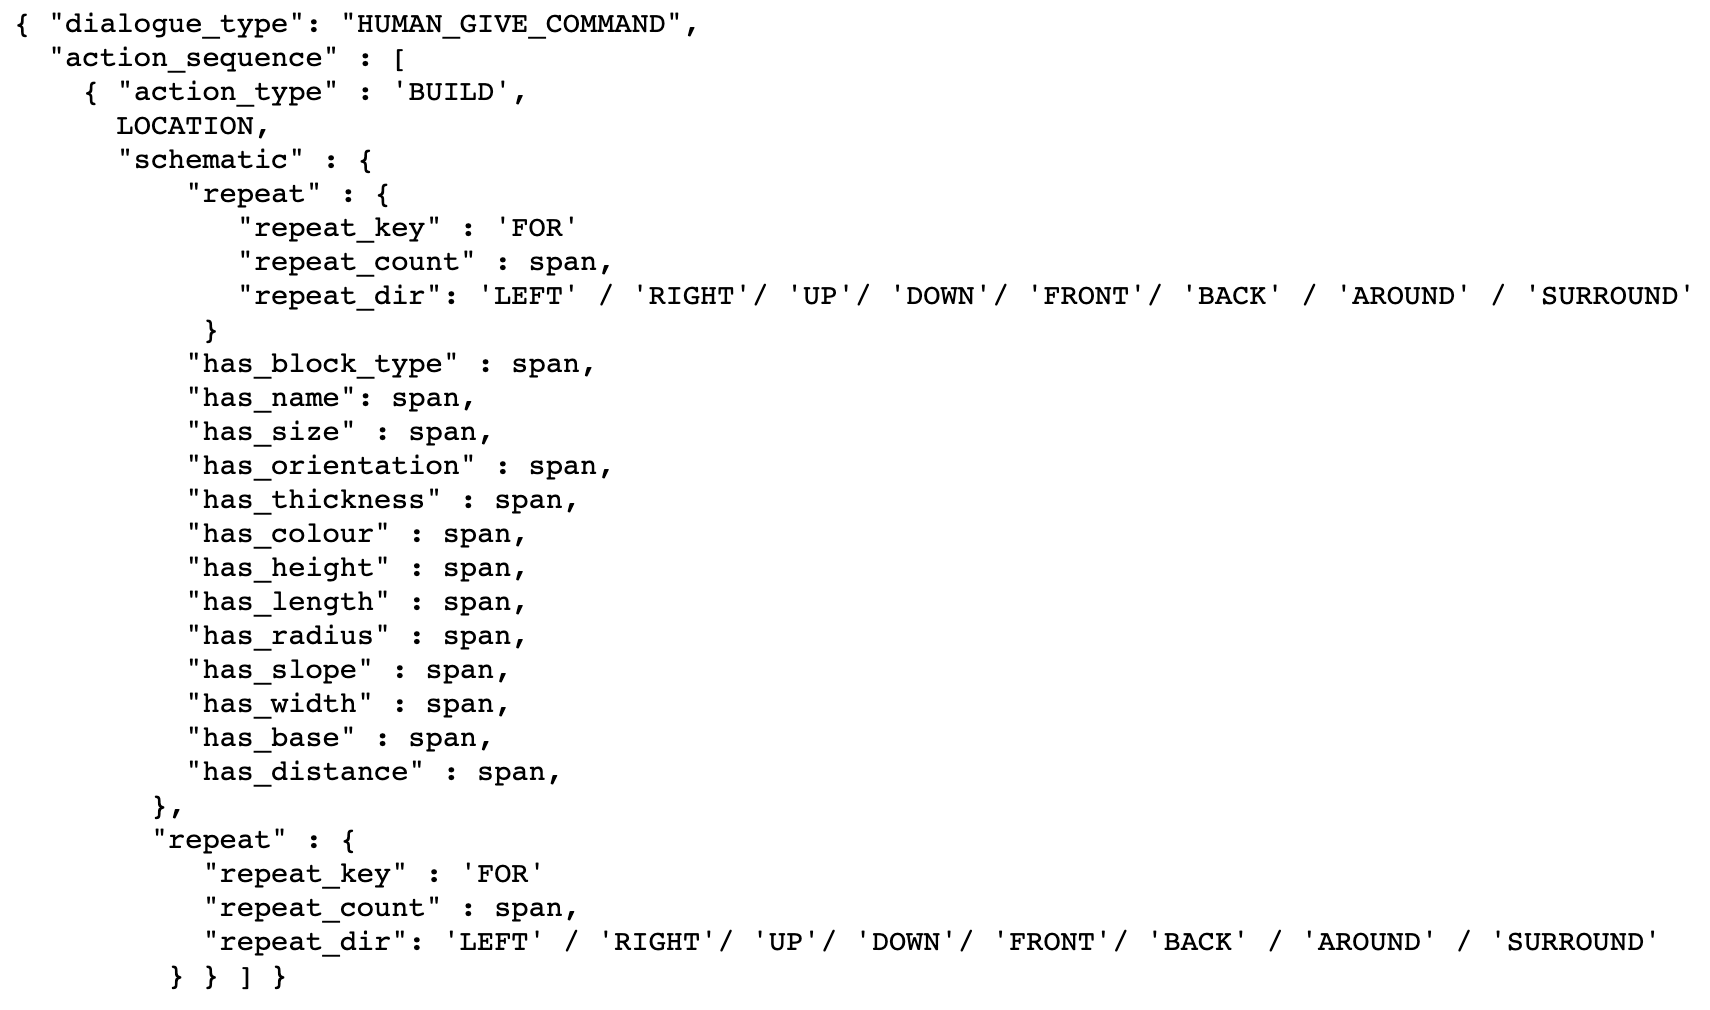
\includegraphics[width=15cm,height=20cm,keepaspectratio]{figures/build.png}
    \caption{Details of logical form for Build}
    \label{fig:build_dict}
\end{figure}

\subsection{Copy Action}
This is the action to copy a block object to an optional location. The copy action is represented as a "Build" with an optional "reference object" . The logical form  is shown in \ref{fig:copy_dict}.

\begin{figure}[h]
    \centering
    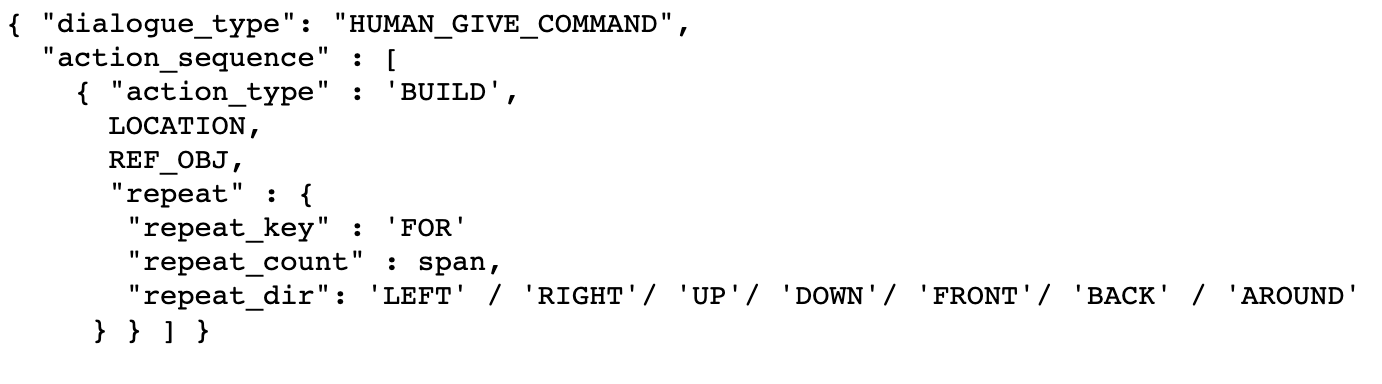
\includegraphics[width=15cm,height=20cm,keepaspectratio]{figures/copy.png}
    \caption{Details of logical form for Copy}
    \label{fig:copy_dict}
\end{figure}

\subsection{ Spawn Action}
This action indicates that the specified object should be spawned in the environment. The logical form is shown in: \ref{fig:spawn_dict}

\begin{figure}[h]
    \centering
    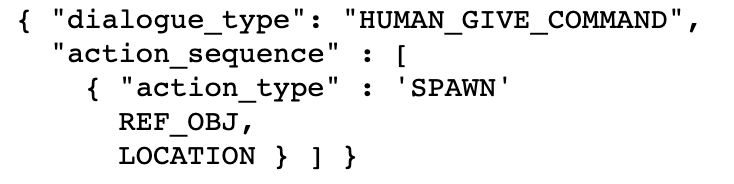
\includegraphics[width=8cm,height=10cm,keepaspectratio]{figures/spawn.png}
    \caption{Details of logical form for Spawn action}
    \label{fig:spawn_dict}
\end{figure}


\subsection{ Fill Action}
This action states that a hole / negative shape at an optional location needs to be filled up. The logical form  is explained in : \ref{fig:fill_dict}

\begin{figure}[h]
    \centering
    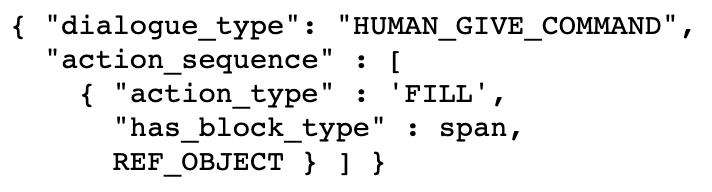
\includegraphics[width=8cm,height=20cm,keepaspectratio]{figures/fill.png}
    \caption{Details of logical form  for Fill}
    \label{fig:fill_dict}
\end{figure}

\subsection{ Destroy Action}
This action indicates the intent to destroy a block object at an optional location. The logical form  is shown in: \ref{fig:destroy_dict}

Destroy action can have one of the following as the child:
\begin{itemize}
	\setlength\itemsep{0.0em}
	\item reference object
	\item nothing
\end{itemize}
\begin{figure}[h]
    \centering
    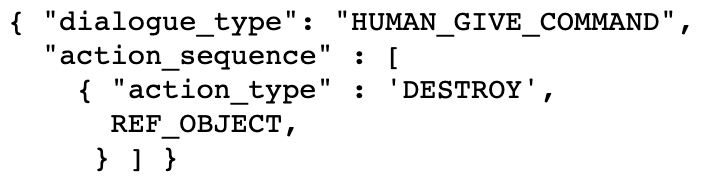
\includegraphics[width=8cm,height=20cm,keepaspectratio]{figures/destroy.png}
    \caption{Details of logical form  Destroy} 
    \label{fig:destroy_dict}
\end{figure}

\subsection{Move Action}
This action states that the agent should move to the specified location, the corresponding logical form  is in: \ref{fig:move_dict}

Move action can have one of the following as its child:
\begin{itemize}
	\setlength\itemsep{0.0em}
	\item location
	\item stop condition (stop moving when a condition is met)
	\item location and stop condition
	\item neither
\end{itemize}
\begin{figure}[h]
    \centering
    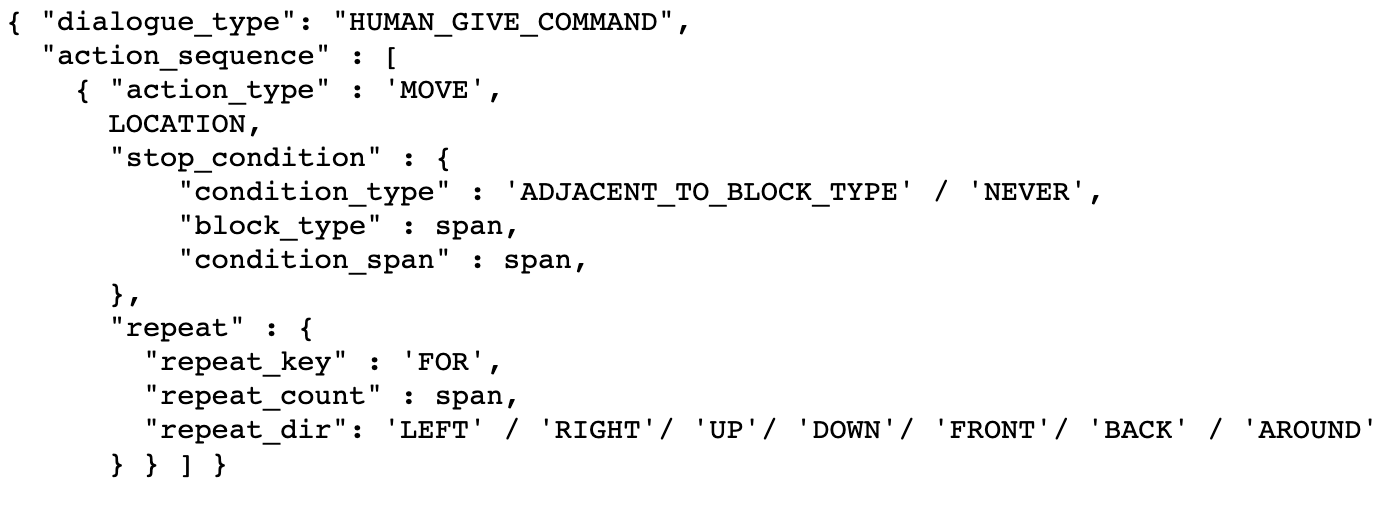
\includegraphics[width=15cm,height=20cm,keepaspectratio]{figures/move.png}
    \caption{Details of logical form  for Move action}
    \label{fig:move_dict}
\end{figure}

\subsection{ Dig Action}
This action represents the intent to dig a hole / negative shape of optional dimensions at an optional location. The logical form is in \ref{fig:dig_dict}

\begin{figure}[h]
    \centering
    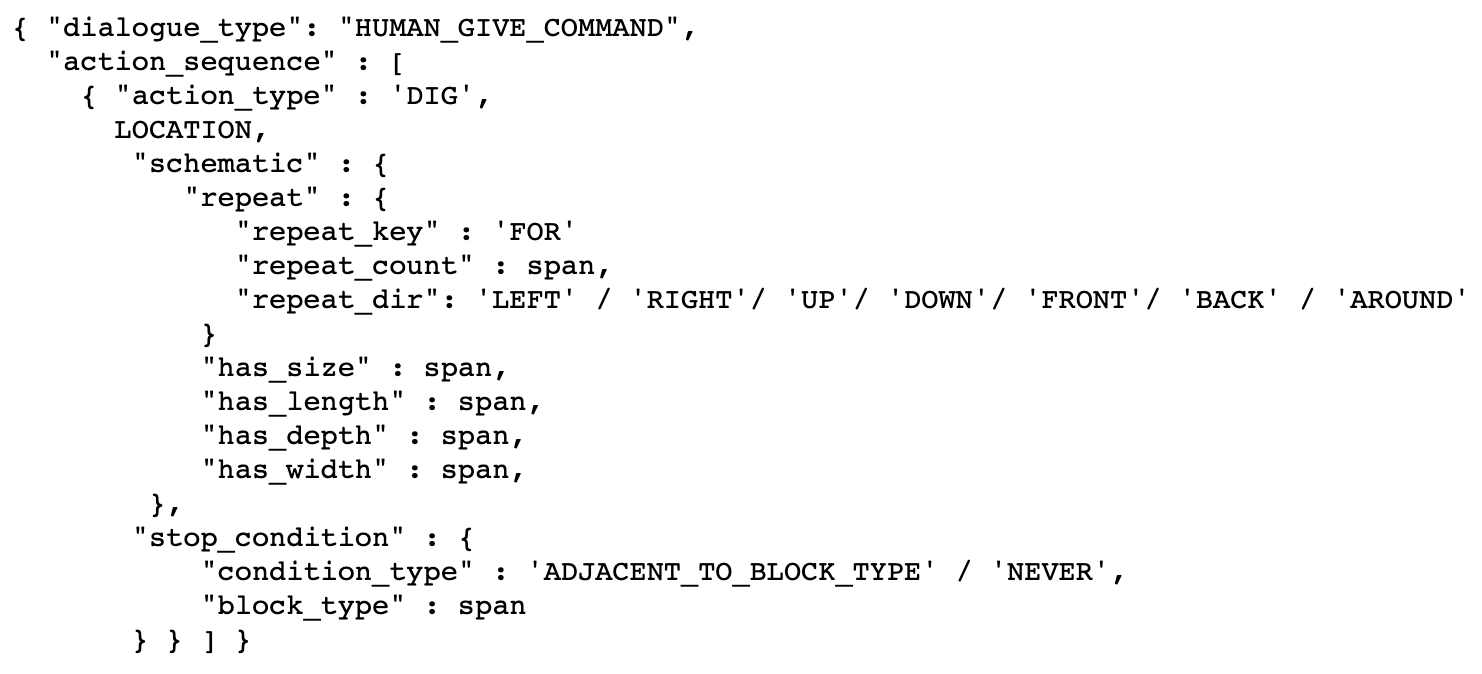
\includegraphics[width=15cm,height=20cm,keepaspectratio]{figures/dig.png}
    \caption{Details of logical form for Dig action}
    \label{fig:dig_dict}
\end{figure}

\subsection{Dance Action}
This action represents that the agent performs a movement of a certain kind. Note that this action is different than a Move action in that the path or step-sequence here is more important than the destination. The logical form is shown in \ref{fig:dance_dict}

\begin{figure}[h]
    \centering
    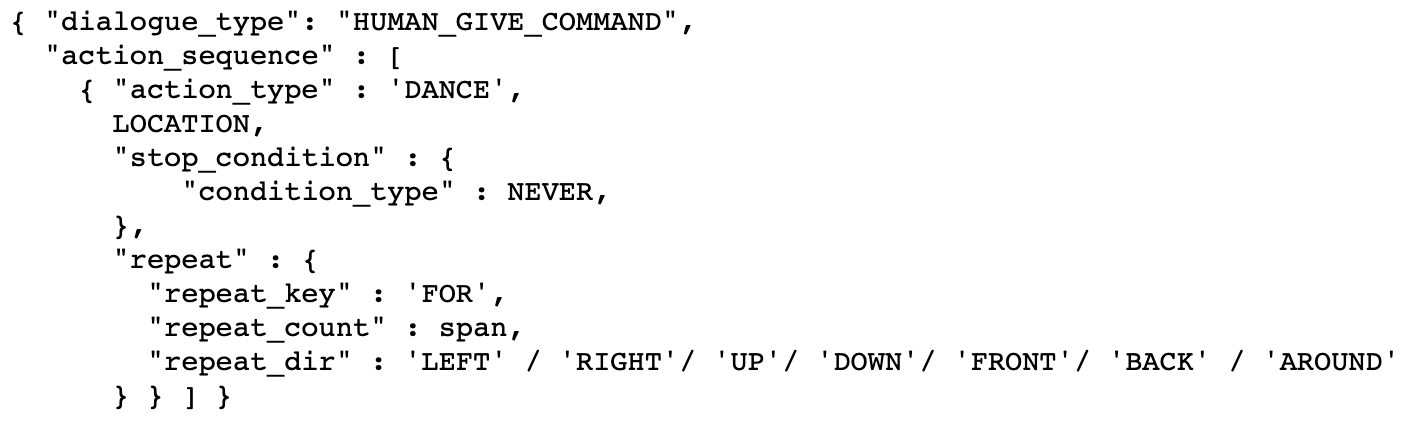
\includegraphics[width=15cm,height=20cm,keepaspectratio]{figures/dance.png}
    \caption{Details of logical form for Dance action}
    \label{fig:dance_dict}
\end{figure}

\subsection{FreeBuild Action}
This action represents that the agent should complete an already existing half-finished block object, using its mental model. The logical form is explained in: \ref{fig:freebuild_dict}

FreeBuild action can have one of the following as its child:
\begin{itemize}
	\setlength\itemsep{0.0em}
	\item reference object only
	\item reference object and location
\end{itemize}

\begin{figure}[h]
    \centering
    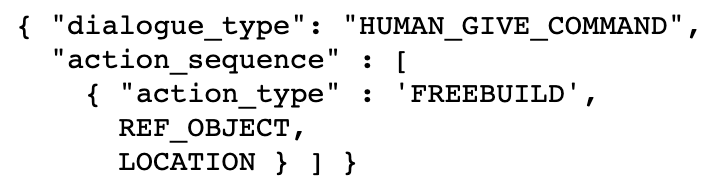
\includegraphics[width=8cm,height=20cm,keepaspectratio]{figures/freebuild.png}
    \caption{Details of logical form for FreeBuild action}
    \label{fig:freebuild_dict}
\end{figure}

\subsection{ Undo Action}
This action states the intent to revert the specified action, if any. The logical form is in \ref{fig:undo_dict}.
Undo action can have on of the following as its child:
\begin{itemize}
	\setlength\itemsep{0.0em}
	\item target\_action\_type 
	\item nothing (meaning : undo the last action)
\end{itemize}
\begin{figure}[h]
    \centering
    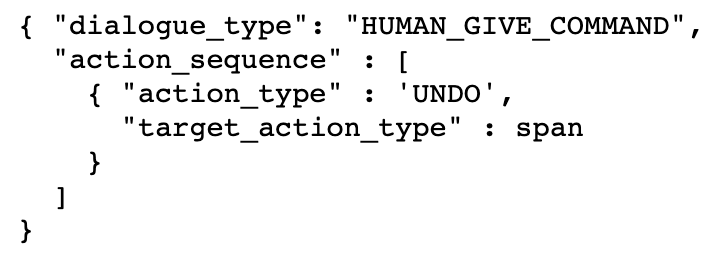
\includegraphics[width=5cm,height=5cm,keepaspectratio]{figures/undo.png}
    \caption{Details of logical form for Undo action}
    \label{fig:undo_dict}
\end{figure}

\subsection{ Stop Action}
This action indicates stop and the logical form is shown in \ref{fig:stop_dict}
\begin{figure}[h]
    \centering
    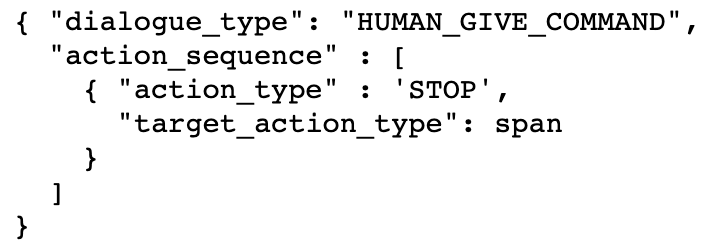
\includegraphics[width=5cm,height=5cm,keepaspectratio]{figures/stop.png}
    \caption{Details of logical form for Stop action}
    \label{fig:stop_dict}
\end{figure}

\subsection{Resume Action}
This action indicates that the previous action should be resumed, the logical form is shown in: \ref{fig:resume_dict}
\begin{figure}[h]
    \centering
    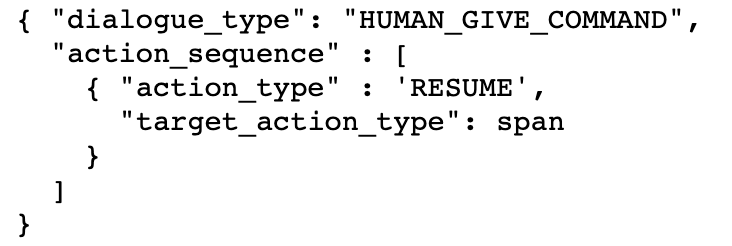
\includegraphics[width=5cm,height=5cm,keepaspectratio]{figures/resume.png}
    \caption{Details of logical form for Resume action}
    \label{fig:resume_dict}
\end{figure}

\subsection{Get Memory Dialogue type}
This dialogue type represents the agent answering a question about the environment.
This is similar to the setup in Visual Question Answering. The logical form is represented in: \ref{fig:answer_dict}

Get Memory dialogue has the following as its children: filters, answer type and tag name.
This dialogue type represents the type of expected answer : counting, querying a specific attribute or querying everything ("what is the size of X" vs "what is X" )
\begin{figure}[h]
    \centering
    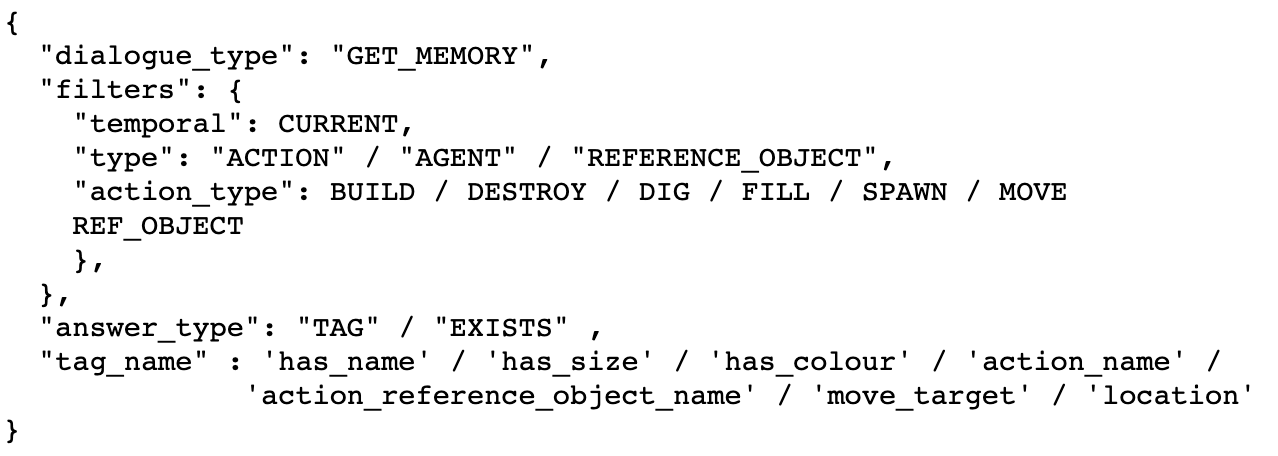
\includegraphics[width=12cm,height=12cm,keepaspectratio]{figures/answer.png}
    \caption{Details of logical form for Get Memory Dialogue}
    \label{fig:answer_dict}
\end{figure}


\subsection{Put Memory Dialogue}
This dialogue type represents that a reference object should be tagged with the given tag and the logical form is shown in: \ref{fig:tag_dict}

\begin{figure}[h]
    \centering
    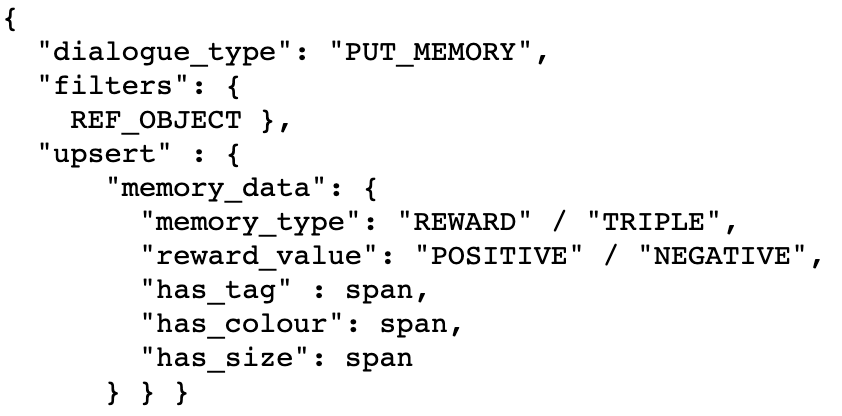
\includegraphics[width=10.8cm,height=15cm,keepaspectratio]{figures/tag.png}
    \caption{Details of logical form for Put Memory Dialogue}
    \label{fig:tag_dict}
\end{figure}


\subsection{ Noop Dialogue}
This dialogue type indicates no operation should be performed, the logical form is shown in : \ref{fig:noop_dict}
\begin{figure}[h]
	\centering
    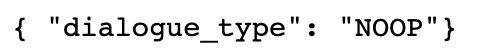
\includegraphics[width=5cm,height=5cm,keepaspectratio]{figures/noop.png}
    \caption{Details of logical form for Noop Dialogue}
    \label{fig:noop_dict}
\end{figure}


\clearpage

\lstset{
basicstyle=\small\ttfamily,
columns=flexible,
breaklines=true
}

\section{Crowd-sourced task and tools instructions}
\label{sec:dataset_examples}

Some examples from prompts data:

\begin{lstlisting}[language=TeX]

bot move the tree to the left side of the house
{'action_sequence': [{
  'action_type': 'OTHERACTION',
  'location': {
    'location_type': 'REFERENCE_OBJECT',
    'reference_object': {
      'has_name': [0, [10, 10]]},
    'relative_direction': 'LEFT'},
  'reference_object': {
    'has_name': [0, [3, 3]]}}],
 'dialogue_type': 'HUMAN_GIVE_COMMAND'}

dig a hole next to that house
{'action_sequence': [{
  'action_type': 'DIG',
  'location': {
     'location_type': 'REFERENCE_OBJECT',
     'reference_object': {
        'contains_coreference': 'yes',
        'has_name': [0, [6, 6]]},
     'relative_direction': 'NEAR'},
  'schematic': {
    'has_name': [0, [2, 2]]}}],
 'dialogue_type': 'HUMAN_GIVE_COMMAND'}

how about you copy the crops i planted to fill this whole plain
{'action_sequence': [{
  'action_type': 'BUILD',
  'reference_object': {
     'has_name': [0, [5, 5]],
     'has_tag': [0, [6, 7]]},
  'repeat': {
     'stop_condition': {
       'condition_span': [0, [9, 12]]}}}],
 'dialogue_type': 'HUMAN_GIVE_COMMAND'}

make sure i spawn on top of the pyramid each time
{'action_sequence': [{
  'action_type': 'OTHERACTION',
  'location': {
    'location_type': 'REFERENCE_OBJECT',
    'reference_object': {
      'has_name': [0, [8, 8]]},
    'relative_direction': 'UP'},
  'reference_object': {
    'has_name': [0, [2, 2]]},
  'repeat': {'stop_condition': {'condition_type': 'NEVER'}}}],
 'dialogue_type': 'HUMAN_GIVE_COMMAND'}

complete the structure 10 meters west from your position
{'action_sequence': [{
  'action_type': 'FREEBUILD',
  'reference_object': {
    'has_name': [0, [2, 2]],
    'location': {
      'location_type': 'AGENT_POS',
      'relative_direction': 'LEFT',
      'steps': [0, [3, 3]]}}}],
 'dialogue_type': 'HUMAN_GIVE_COMMAND'}

destroy the structure that is blocking the view of the landscape
{'action_sequence': [{
  'action_type': 'DESTROY',
  'reference_object': {
    'has_name': [0, [2, 2]],
    'has_tag': [0, [5, 10]]}}],
 'dialogue_type': 'HUMAN_GIVE_COMMAND'}

complete the project that i am working on by building more devices
{'action_sequence': [{
  'action_type': 'FREEBUILD',
  'reference_object': {
    'has_name': [0, [2, 2]],
    'has_tag': [0, [4, 7]]}}],
 'dialogue_type': 'HUMAN_GIVE_COMMAND'}

show me how to dance
{'action_sequence': [{
  'action_type': 'DANCE'}],
 'dialogue_type': 'HUMAN_GIVE_COMMAND'}

please build a garden
{'action_sequence': [{
  'action_type': 'BUILD',
  'schematic': {
     'has_name': [0, [3, 3]]}}],
 'dialogue_type': 'HUMAN_GIVE_COMMAND'}

fill the small pond with sand
{'action_sequence': [{
  'action_type': 'FILL',
  'has_block_type': [0, [5, 5]],
  'reference_object': {
    'has_name': [0, [3, 3]],
    'has_size': [0, [2, 2]]}}],
 'dialogue_type': 'HUMAN_GIVE_COMMAND'}

move north for 5 minutes
{'action_sequence': [{
  'action_type': 'MOVE',
  'location': {
    'location_type': 'AGENT_POS',
    'relative_direction': 'FRONT'},
  'repeat': {
    'stop_condition': {
      'condition_span': [0, [3, 4]]}}}],
 'dialogue_type': 'HUMAN_GIVE_COMMAND'}

dig a hole next to the sidewalk of the school
{'action_sequence': [{
  'action_type': 'DIG',
  'location': {
    'location_type': 'REFERENCE_OBJECT',
    'reference_object': {
      'has_name': [0, [6, 9]]},
    'relative_direction': 'NEAR'},
  'schematic': {'has_name': [0, [2, 2]]}}],
 'dialogue_type': 'HUMAN_GIVE_COMMAND'}

move to the right until you ca n't anymore
{'action_sequence': [{
  'action_type': 'MOVE',
  'location': {
    'location_type': 'SPEAKER_POS',
    'relative_direction': 'RIGHT'},
  'repeat': {
    'stop_condition': {
      'condition_span': [0, [4, 8]]}}}],
 'dialogue_type': 'HUMAN_GIVE_COMMAND'}

move up the hill
{'action_sequence': [{
  'action_type': 'MOVE',
  'location': {
    'location_type': 'REFERENCE_OBJECT',
    'reference_object': {
      'has_name': [0, [3, 3]]},
    'relative_direction': 'UP'}}],
 'dialogue_type': 'HUMAN_GIVE_COMMAND'}

build a bridge over the lava
{'action_sequence': [{
  'action_type': 'BUILD',
  'location': {
    'location_type': 'REFERENCE_OBJECT',
    'reference_object': {
       'has_name': [0, [5, 5]]},
    'relative_direction': 'UP'},
  'schematic': {'has_name': [0, [2, 2]]}}],
 'dialogue_type': 'HUMAN_GIVE_COMMAND'}

this pyramid is 5 platforms tall
{'dialogue_type': 'NOOP'}

spawn 30 cows and build a 15 by 15 fence
{'action_sequence': [
  {
  'action_type': 'SPAWN',
  'reference_object': {
    'has_name': [0, [2, 2]]},
   'repeat': {
     'repeat_count': [0, [1, 1]],
     'repeat_key': 'FOR'}},
  {
  'action_type': 'BUILD',
  'schematic': {
    'has_height': [0, [2, 2]],
    'has_name': [0, [5, 5]]}}],
 'dialogue_type': 'HUMAN_GIVE_COMMAND'}

move three feet forward and stop
{'action_sequence': [{
  'action_type': 'MOVE',
  'location': {
    'location_type': 'AGENT_POS',
    'relative_direction': 'FRONT',
    'steps': [0, [1, 2]]}}],
 'dialogue_type': 'HUMAN_GIVE_COMMAND'}

destroy the building that 's in front of you
{'action_sequence': [{
  'action_type': 'DESTROY',
  'reference_object': {
    'has_name': [0, [2, 2]],
    'location': {
      'location_type': 'AGENT_POS',
      'relative_direction': 'FRONT'}}}],
 'dialogue_type': 'HUMAN_GIVE_COMMAND'}

tag the horse armor
{'dialogue_type': 'PUT_MEMORY',
 'filters': {
   'reference_object': {
     'has_name': [0, [2, 3]]}}}

bot build it to fit into the open frame
{'action_sequence': [{
  'action_type': 'BUILD',
  'schematic': {
    'has_name': [0, [2, 2]],
    'has_tag': [0, [4, 8]]}}],
 'dialogue_type': 'HUMAN_GIVE_COMMAND'}

destroy the hut near the big tree
{'action_sequence': [{
  'action_type': 'DESTROY',
  'reference_object': {
     'has_name': [0, [2, 2]]}}],
 'dialogue_type': 'HUMAN_GIVE_COMMAND'}

move the rabbit into the box
{'action_sequence': [{
  'action_type': 'OTHERACTION',
  'location': {
    'location_type': 'REFERENCE_OBJECT',
    'reference_object': {
       'has_name': [0, [5, 5]]},
    'relative_direction': 'INSIDE'},
  'reference_object': {'has_name': [0, [2, 2]]}}],
 'dialogue_type': 'HUMAN_GIVE_COMMAND'}

fill the entire tub with pepsi
{'action_sequence': [{
  'action_type': 'FILL',
  'has_block_type': [0, [5, 5]],
  'reference_object': {
    'has_name': [0, [3, 3]]}}],
 'dialogue_type': 'HUMAN_GIVE_COMMAND'}

stop digging
{'action_sequence': [{
  'action_type': 'STOP',
  'target_action_type': [0, [1, 1]]}],
 'dialogue_type': 'HUMAN_GIVE_COMMAND'}

destroy the box
{'action_sequence': [{
  'action_type': 'DESTROY',
  'reference_object': {
    'has_name': [0, [2, 2]]}}],
 'dialogue_type': 'HUMAN_GIVE_COMMAND'}

let 's resume our mission of traveling over that treacherous mountain pass
{'action_sequence': [{
  'action_type': 'RESUME',
  'target_action_type': [0, [3, 11]]}],
 'dialogue_type': 'HUMAN_GIVE_COMMAND'}

build a house with a porch next to the pyramid
{'action_sequence': [{
  'action_type': 'BUILD',
  'location': {
    'location_type': 'REFERENCE_OBJECT',
    'reference_object': {
      'has_name': [0, [9, 9]]},
    'relative_direction': 'NEAR'},
  'schematic': {
    'has_name': [0, [2, 2]],
    'has_tag': [0, [3, 5]]}}],
 'dialogue_type': 'HUMAN_GIVE_COMMAND'}

build stairs in the corner
{'action_sequence': [{
  'action_type': 'BUILD',
  'location': {
    'location_type': 'REFERENCE_OBJECT',
    'reference_object': {
      'has_name': [0, [4, 4]]}},
  'schematic': {
    'has_name': [0, [1, 1]]}}],
 'dialogue_type': 'HUMAN_GIVE_COMMAND'}

spawn milk
{'action_sequence': [{
  'action_type': 'SPAWN',
  'reference_object': {
    'has_name': [0, [1, 1]]}}],
 'dialogue_type': 'HUMAN_GIVE_COMMAND'}

build a wall to divide the largest room in the house
{'action_sequence': [{
  'action_type': 'BUILD',
  'location': {
    'location_type': 'REFERENCE_OBJECT',
    'reference_object': {
       'has_name': [0, [6, 10]]},
    'relative_direction': 'INSIDE'},
  'schematic': {'has_name': [0, [2, 2]]}}],
 'dialogue_type': 'HUMAN_GIVE_COMMAND'}

build foundation
{'action_sequence': [{
  'action_type': 'BUILD',
  'schematic': {
    'has_name': [0, [1, 1]]}}],
 'dialogue_type': 'HUMAN_GIVE_COMMAND'}

please change the barn to a shop
{'action_sequence': [{
  'action_type': 'OTHERACTION',
  'reference_object': {
    'has_name': [0, [3, 3]]}}],
 'dialogue_type': 'HUMAN_GIVE_COMMAND'}

copy the loaf of bread 100 times for distribution to the assembled army in front of you
{'action_sequence': [{
  'action_type': 'BUILD',
  'reference_object': {
    'has_name': [0, [2, 4]]},
  'repeat': {
    'repeat_count': [0, [5, 5]],
    'repeat_key': 'FOR'}}],
 'dialogue_type': 'HUMAN_GIVE_COMMAND'}

spawn fifteen horses
{'action_sequence': [{
  'action_type': 'SPAWN',
  'reference_object': {
    'has_name': [0, [2, 2]]},
  'repeat': {
    'repeat_count': [0, [1, 1]],
    'repeat_key': 'FOR'}}],
 'dialogue_type': 'HUMAN_GIVE_COMMAND'}

dance
{'action_sequence': [{
  'action_type': 'DANCE'}],
 'dialogue_type': 'HUMAN_GIVE_COMMAND'}

dig a hole beneath the fence on the west side of the prison yard big enough for a person to crawl through
{'action_sequence': [{
  'action_type': 'DIG',
  'location': {
    'location_type': 'REFERENCE_OBJECT',
    'reference_object': {
       'has_name': [0, [5, 13]]},
    'relative_direction': 'DOWN'},
  'repeat': {
    'stop_condition': {
      'condition_span': [0, [14, 21]]}},
  'schematic': {
    'has_name': [0, [2, 2]]}}],
 'dialogue_type': 'HUMAN_GIVE_COMMAND'}
\end{lstlisting}
% \clearpage

\section{Analysis of errors on prompts and interactive data}
\label{sec:analysis_prompts}

We performed error analysis on the mistakes that the model made. Table ~\ref{tab:action-type} shows the accuracy scores per action-type for the SentenceRec model.
\begin{table*}
\small
\center
\begin{tabular}{c|cccc|cccc}
	& \multicolumn{4}{c|}{Validation} 	& \multicolumn{4}{c}{Test} \\
Action Type 	& Temp.	&	Rep.	&	Prompts	&	Inter.	&	Temp.	& Rep. 	&	Prompts 	&	Inter. \\
\midrule
Answer	&	1.000	&	0.758	& \textbf{0.000	}	&	\textbf{0.000}	&	1.000	&	0.859	&	\textbf{0.000}	&	\textbf{0.000} \\
\midrule
 Build	&	0.983	&	0.725	&	0.417	&	0.705	&	0.979	&	0.763	&	0.396	&	0.667 \\
 \midrule
 Destroy	&	0.985	&	0.777	&	0.185	&	0.560	&	0.972	&	0.787	&	0.241	&	0.406 \\
 \midrule
 Dig	&	1.000	&	0.781	&	0.382	&	0.462	&	0.995	&	0.797	&	0.389	&	0.667 \\
 \midrule
 Fill	&	1.000	&	0.782	&	0.111	&	0.000	&	0.995	&	0.806	&	0.083	&	0.500 \\
 \midrule
 FreeBuild	&	0.993	&	0.779	&	\textbf{0.000}	&	\textbf{0.000}	&	0.987	&	0.747	&	\textbf{0.000}	&	\textbf{0.000} \\
 \midrule
 Move	&	1.000	&	0.768	&	0.419	&	0.357	&	1.000	&	0.707	&	0.269	&	0.455 \\
 \midrule
 Noop	&	0.952	&	0.970	&	0.800	&	0.878	&	0.963	&	0.960	&	0.685	&	0.861 \\
 \midrule
 Resume	&	1.000	&	0.857	&	0.486	&	1.000	&	1.000	&	0.956	&	0.625	&	1.000 \\
 \midrule
 Stop		&	1.000	&	0.979	&	0.829	&	0.750	&	1.000	&	0.880	&	0.744	&	1.000 \\
 \midrule
 Tag	&	0.995	&	0.708	&	\textbf{0.000}	&	\textbf{0.000}	&	0.988	&	0.709	&	\textbf{0.000}	&	\textbf{0.000} \\
 \midrule
 Undo	&	1.000	&	0.817	&	0.462	&	N/A	&	1.000	&	0.782	&	0.632	&	1.000 \\
 \midrule
 CompositeAction	&	N/A	&	N/A	&	\textbf{0.000}	&	N/A	&	N/A	&	N/A	&	\textbf{0.000}	&	N/A \\
 \midrule
 OtherAction	&	N/A	&	N/A	&	\textbf{0.000}	&	\textbf{0.000}	&	N/A	&	N/A	&	\textbf{0.000}	&	\textbf{0.000} \\

\end{tabular}
\caption{Action type accuracy breakdown for the SentenceRec model over the validation and test datasets. 'N/A' refers to the action type not found in that dataset. }
\label{tab:action-type}
\end{table*}

We conclude from Table ~\ref{tab:action-type} that the model makes most mistakes on prompts and interactive data. We found that the parsing model does poorly on specifically : Answer, CompositeAction, OtherAction, Destroy, FreeBuild and Tag actions. The following sections go into a deeper understanding of the errors.

\subsection{Answer action}
The Answer action errors can be categorized into the following:
\begin{itemize}
\item A significant portion of the errors in Answer happens because crowd-sourced workers annotated the action with just an ``answer\_type" key, however the model tries to predict more details for the object being referred to, example:
\begin{verbatim}
sentence: "what is this" 
ground truth tree: {"action_type" :  "Answer"}
prediction tree :{
"reference_object": {
    "location": {"location_type": "SpeakerLook"}}, 
"action_type": "Answer", 
"answer_type": "query_all_tags"
}
\end{verbatim}
another example:
\begin{verbatim}
sentence: "what do you think is under this pyramid ?"
ground truth tree: {"action_type": "Answer"}
prediction tree : {
"reference_object": {
    "location": {
	    "reference_object": {
		    "location": {"location_type": "SpeakerLook"}, 
		    "has_name_": (0, (7, 7))}, 
        "location_type": "ReferenceObject",
        "relative_direction": "DOWN"}}, 
"action_type": "Answer", 
"answer_type": "query_all_tags"}
\end{verbatim}

\item Some commands have been tagged as ``Answer" by humans but model predicts them as other action types, example:
\begin{verbatim}
sentence: "can we build a garden"
ground truth tree: {"action_type": "Answer"}
prediction tree : {
"schematic": {
    "has_name_": (0, (4, 4))}, 
"action_type": "Build"}
\end{verbatim}

\item Some are ambiguous and can be classified as either, example:
\begin{verbatim}
sentence: "can you chop down that tree for me ?"
ground truth tree: {"action_type": "Answer"}
prediction tree : {
"reference_object": {
    "location": {"location_type": "SpeakerLook"},
     "has_name_": (0, (5, 5))}, 
"action_type": "Destroy"}
\end{verbatim}

\item Some are out of distribution questions, example:
\begin{verbatim}
sentence: "what can you tag"
ground truth tree: {"action_type": "Answer"}
prediction tree : {
"action_type": "Undo, 
"undo_action": "Tag_Action"
}
\end{verbatim}
\end{itemize}

\subsection{Tag action}
The main category of errors in the Tag action is commands that have no reference objects example:
\begin{verbatim}
sentence: "label as grass"
ground truth tree: {
"tag": [2, 2], 
"action_type": "Tag"}
prediction tree : {
"reference_object": {
    "has_name_": (0, (2, 2))}, 
"action_type": "Tag", 
"tag": (0, (2, 2))}
\end{verbatim}

In the training data, the model always sees commands that try to tag some object.

\subsection{FreeBuild action}
The Freebuild mistakes fall into two major categories:
\begin{itemize}
\item Distinction between FreeBuild and Build is ambiguous, example:
\begin{verbatim}
sentence: "ok build me a house with me"
ground truth tree: {
"schematic": {
    "has_name_": [4, 4]}, 
"action_type": "FreeBuild"}
prediction tree : {"action_type": "Build"}
\end{verbatim}
These are new kinds of commands for the FreeBuild action that the model doesn't see in training data and the action type can be easily confused with ``Build"
\item Distinction between FreeBuild and Resume is ambiguous, example:
\begin{verbatim}
sentence: "continue building the house"
ground truth tree: {
"schematic": {
    "has_name_": [3, 3]}, 
"action_type": "FreeBuild"}
prediction tree : {"action_type": "Resume"}
\end{verbatim}
These commands can be easily (and perhaps correctly) confused with Resume action.
\end{itemize}
 
 \subsection{OtherAction and CompositeAction}
 The models do very poorly on these action types as they never see these actions in the training data. 
 These actions represent all the commands that do not fall into the category of defined commands in the training data and the data points are too few for these action types. 
 
 \begin{itemize}
 \item Ambiguous action types:
 \begin{verbatim}
 sentence: 'stop the car .'
ground truth tree: {
'reference_object': {
    'has_name_': [2, 2]}, 
'action_type': 'OtherAction'}
prediction tree : {'action_type': 'Stop'}
\end{verbatim}
This can be correctly classified as Stop action. There's a bunch of these in the data for other action types like Build, Fill etc
\item There are a lot of `annotation errors:
\begin{verbatim}
sentence: 'spawn a garden .'
ground truth tree: {
'reference_object': {
    'has_name_': [2, 2]}, 
'action_type': 'OtherAction'}
prediction tree : {
'schematic': {
    'has_name_': (0, (2, 2))}, 
'action_type': 'Build'}
\end{verbatim}
 \end{itemize}

 \subsection{Other Errors}
 \begin{itemize}
 \item Sometimes the model gets more details than ground truth annotations :
\begin{verbatim}
sentence: "build a fortified base"
ground truth tree: {
"schematic": {
    "has_name_": [2, 3]}, 
"action_type": "Build"}
prediction tree : {
"schematic": {
    "has_name_": (0, (3, 3)), 
    "has_block_type_": (0, (2, 2))}, 
"action_type": "Build"}
\end{verbatim}
\item Out of training distribution commands:

\begin{verbatim}
sentence: "demolish the guest house in the backyard ."
ground truth tree: {
"location": {
    "location_type": "ReferenceObject", 
    "reference_object": {
        "has_name_": [6, 6]}}, 
"reference_object": {
    "has_name_": [2, 3]}, 
"action_type": "Destroy"}
prediction tree : {
"reference_object": {
    "has_name_": (0, (2, 2))},
"action_type": "Destroy"}
\end{verbatim}
The model doesn't see location descriptions that are described by ``in" in the training data.
 \end{itemize}



\end{document}
